\documentclass[UTF8,a4paper,12pt]{ctexart}
\usepackage{amsmath,amssymb,amsfonts}
\usepackage{booktabs}
\usepackage{graphicx}
\usepackage{float}
\usepackage{geometry}
\usepackage{longtable}
\usepackage{array}
\usepackage{multirow}
\usepackage{caption}
\usepackage{subcaption}
\usepackage{enumitem}
\usepackage{xcolor}
\usepackage[colorlinks=false,pdfborder={0 0 0}]{hyperref}
\usepackage{setspace}
\usepackage{algorithm}
\usepackage{algpseudocode}
\usepackage{fancyhdr}
\usepackage{listings}

\geometry{left=2.5cm,right=2.5cm,top=2.5cm,bottom=2.5cm}
\onehalfspacing
\setlength{\parindent}{2em}
\captionsetup{font=small,labelsep=space}
\pagestyle{fancy}
\fancyhf{}
\fancyhead[C]{古代玻璃制品的成分分析与鉴别}
\fancyfoot[C]{\thepage}
\renewcommand{\headrulewidth}{0.4pt}

\lstset{
  language=Python,
  basicstyle=\ttfamily\scriptsize,
  breaklines=true,
  frame=single,
  numbers=left,
  numberstyle=\tiny\color{gray}
}

\begin{document}

\thispagestyle{plain}
\setcounter{page}{1}
\begin{center}
{\Large\bfseries 古代玻璃制品的成分分析与鉴别}
\end{center}
\vspace{0.4em}
\begin{center}
{\large\bfseries 摘要}
\end{center}
\vspace{0.2em}
{\small
\setlength{\parindent}{2em}
围绕古代玻璃文物的\textbf{成分分析}与\textbf{类型鉴别}，本文在成分性和效口径（成分和∈\textbf{85\%}–\textbf{105\%}）下，构建“\textbf{评价风化}—\textbf{筛选分类}—\textbf{优化亚类}—\textbf{鉴别未知}—\textbf{比较关联}—\textbf{闭环检验}”主线。数据含文物\textbf{58}件（高钾\textbf{18}、铅钡\textbf{40}），成分样本\textbf{69}个，有效\textbf{67}个，无效\textbf{2}个；未知类别\textbf{8}个。

问题1先检验表面风化与\textbf{类型}、\textbf{纹饰}、\textbf{颜色}的关联：\textbf{类型}与风化（\textbf{Chi2}，p=\textbf{0.0195}，V=\textbf{0.344}）；\textbf{纹饰}与风化（\textbf{Chi2}，p=\textbf{0.0839}，V=\textbf{0.292}）；\textbf{颜色}与风化（\textbf{Chi2}，p=\textbf{0.3071}，V=\textbf{0.403}）。结果表明铅钡更易风化（风化率\textbf{70.00\%}），高钾风化率\textbf{33.33\%}。进一步按类型做风化/无风化成分\textbf{Mann-Whitney}检验，显著成分数\textbf{15}；并建立\textbf{类型条件风化因子反演}预测风化前成分，共输出\textbf{32}条预测。相对无校正基线，\textbf{高钾}上因子法相对无校正提升\textbf{56.24\%}，\textbf{铅钡}上因子法相对无校正提升\textbf{54.69\%}。

问题2以\textbf{决策树}、\textbf{随机森林}、\textbf{SVM}与\textbf{化学阈值规则}对照，用\textbf{留一法}评估分类规律。最佳方法为\textbf{化学阈值规则}，LOO准确率\textbf{1.0000}，Macro-F1\textbf{1.0000}；化学规则准确率\textbf{1.0000}。重要成分包括\textbf{PbO}、\textbf{BaO}、\textbf{SiO2}、\textbf{K2O}等。对高钾、铅钡分别做\textbf{K-Means}亚类划分：高钾K=\textbf{2}（轮廓系数\textbf{0.492}），铅钡K=\textbf{4}（轮廓系数\textbf{0.394}）；并以成分相对噪声做灵敏度：噪声\textbf{0}时准确率\textbf{1.0000}，噪声\textbf{10\%}时\textbf{1.0000}。

问题3对未知样本给出\textbf{随机森林}主判定，辅以\textbf{SVM}与规则对照：判定高钾\textbf{3}件、铅钡\textbf{5}件；RF与SVM一致率\textbf{1.000}，RF与规则一致率\textbf{1.000}；平均置信度\textbf{0.933}，最低\textbf{0.840}。在\textbf{5\%}相对噪声蒙特卡洛下平均翻转率\textbf{0.000}，训练留一稳定比例均值\textbf{1.000}。

问题4按类型计算\textbf{Spearman}相关并构建显著相关网络，再用\textbf{Mantel}检验比较结构：r=\textbf{0.1276}，p=\textbf{0.2050}；高钾显著相关对\textbf{32}，铅钡\textbf{40}，平均绝对相关差\textbf{0.377}。最大差异成分对为\textbf{Al2O3}-\textbf{SiO2}。

闭环检验方面，特征消融显示全部主特征LOO=\textbf{1.0000}，仅PbO+BaO为\textbf{1.0000}；分类蒙特卡洛（σ=\textbf{0.08}）准确率均值\textbf{1.0000}，5\%–95\%分位[\textbf{1.0000}, \textbf{1.0000}]，不低于\textbf{0.9}的概率为\textbf{100.00\%}。全文统一符号与成分性约束，强调\textbf{可解释规则}与\textbf{统计学习}互补，以及风化校正对鉴别可靠性的影响。

\vspace{0.5em}
\noindent\textbf{关键词：}古代玻璃；风化校正；随机森林；亚类划分；成分关联
}

\newpage
\pagestyle{fancy}

\section{问题重述}
玻璃是丝绸之路早期贸易往来的重要物证。我国古代玻璃在吸收外来技术后就地取材，外观相似而化学成分不同：铅钡玻璃以铅矿石等为助熔剂，氧化铅、氧化钡含量较高；高钾玻璃以草木灰等含钾物质为助熔剂。古代玻璃易受埋藏环境影响而风化，内部元素与环境元素交换导致成分比例变化，从而干扰类型判断。

附件给出一批已标注为高钾或铅钡的玻璃文物基本信息与化学成分比例，以及若干未知类别样本。成分数据具有成分性，各成分比例累加和理论上应为$100\%$，本题将累加和介于$85\%\sim105\%$的数据视为有效。需要解决：
\begin{enumerate}[leftmargin=2em]
\item 分析表面风化与玻璃类型、纹饰、颜色的关系；结合类型分析有无风化化学成分的统计规律，并根据风化点数据预测风化前成分；
\item 分析高钾与铅钡的分类规律；对每一类选择合适成分做亚类划分，给出方法与结果，并分析合理性与敏感性；
\item 鉴别未知类别样本所属类型，并分析分类结果敏感性；
\item 分析不同类别化学成分关联关系，并比较类别间关联结构的差异性。
\end{enumerate}

\section{问题分析}
\subsection{逻辑主线}
四问构成递进闭环而非并列流水账：先\textbf{评价}风化对成分观测的扭曲（Q1），再在校正后的成分空间中\textbf{筛选}类型判别规则并\textbf{优化}亚类结构（Q2），进而把判别器\textbf{分配}到未知样本并量化不确定性（Q3），最后从关联网络角度解释两类玻璃的工艺/助熔剂差异（Q4）。灵敏度与鲁棒性检验贯穿Q1--Q3，保证结论不只依赖单一点估计。

技术路线见图~\ref{fig:roadmap}。

\begin{figure}[H]
\centering
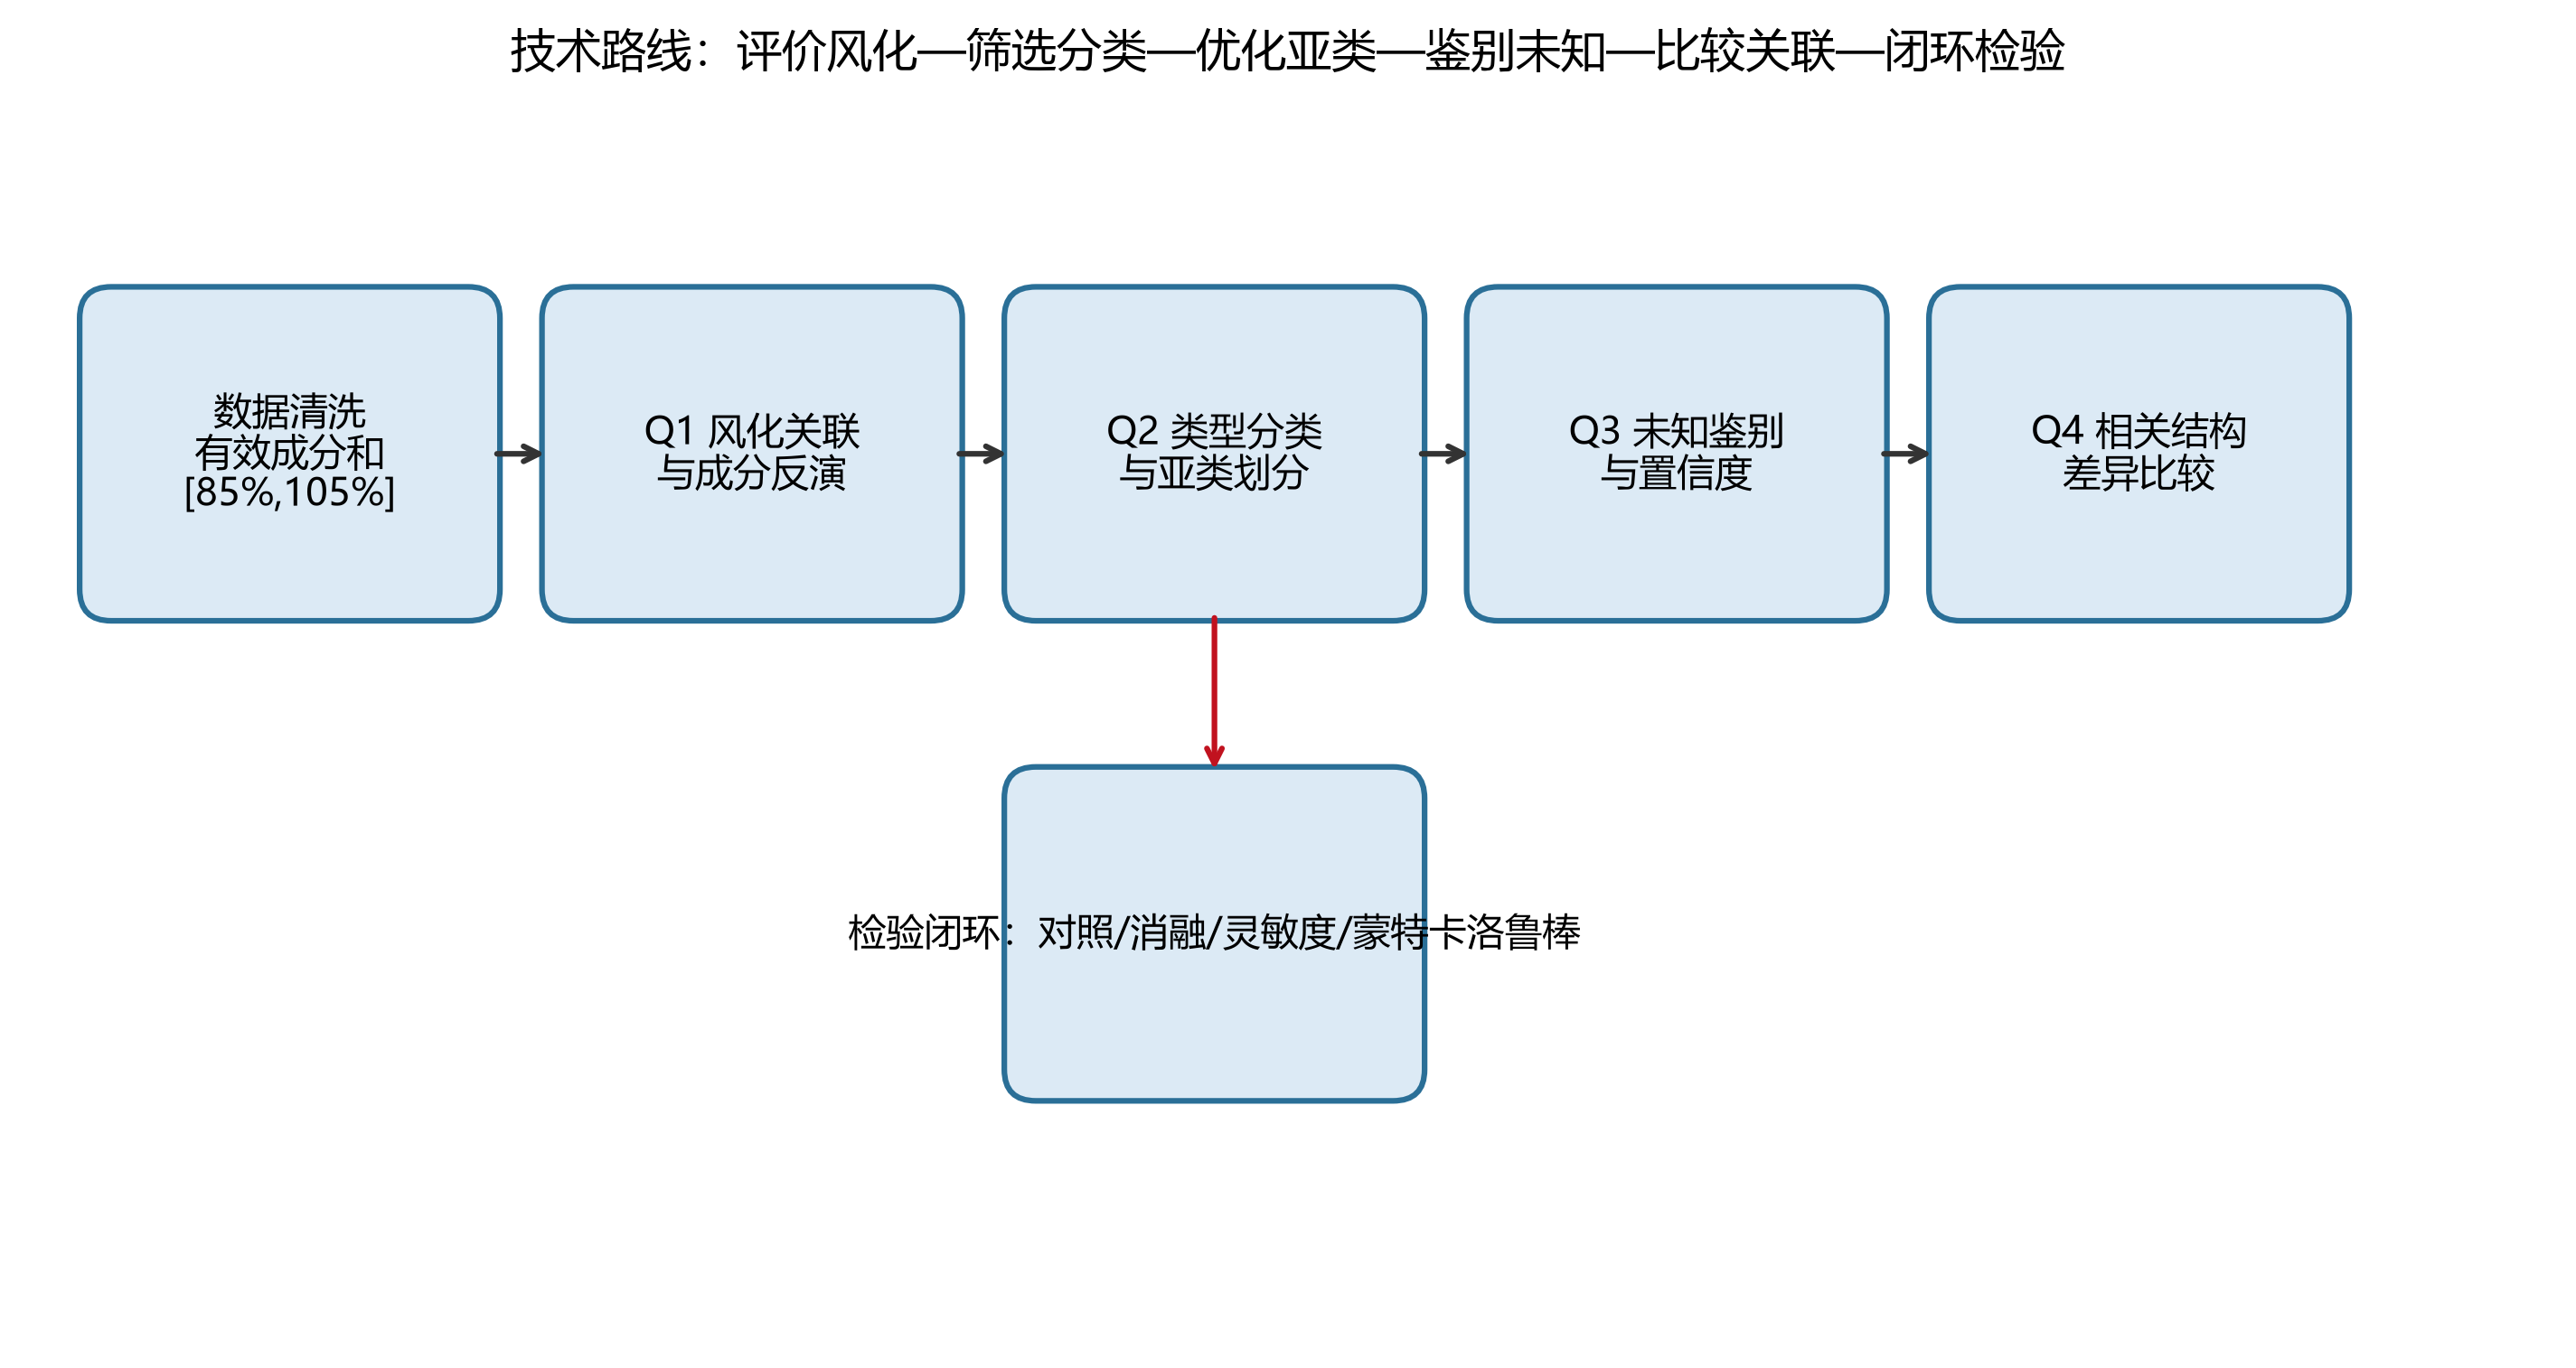
\includegraphics[width=0.98\textwidth]{figures/roadmap_pipeline.png}
\caption{总体技术路线图}
\label{fig:roadmap}
\end{figure}

\subsection{方法选型（国奖向）}
\begin{enumerate}[leftmargin=2em]
\item Q1：列联表$\chi^2$/Fisher + Cramer's $V$；类型分层Mann-Whitney；风化因子反演（主）与差值校正/无校正对照；
\item Q2：可解释化学规则 + 决策树/随机森林/SVM（留一法）；K-Means/层次聚类亚类；噪声与阈值灵敏度；
\item Q3：随机森林概率输出为主，SVM与规则对照；噪声翻转率与训练留一稳定性；
\item Q4：Spearman相关与显著网络；Mantel检验与$|\Delta r|$排序比较结构差异。
\end{enumerate}

\section{模型假设与符号说明}
\subsection{基本假设}
\begin{enumerate}[leftmargin=2em]
\item 表单1的表面风化属性代表该文物采样点的总体风化状态；若采样点标注“未风化点/严重风化点”，则点位标签优先；
\item 空白成分表示未检出，建模时按$0$处理，并在描述统计中报告缺失率；
\item 风化对同类玻璃的平均作用可用成分比值（风化因子）近似刻画，个体差异用灵敏度/鲁棒性评估；
\item 高钾与铅钡在关键助熔剂相关氧化物上可分，允许少量边界样本；
\item 亚类反映类内工艺/配方的连续变异，用轮廓系数选择聚类数。
\end{enumerate}

\subsection{符号说明}
\begin{table}[H]
\centering
\caption{主要符号说明}
\begin{tabular}{cl}
\toprule
符号 & 含义 \\
\midrule
$i$ & 样本索引 \\
$c\in\mathcal{C}$ & 化学成分（SiO$_2$, K$_2$O, PbO, BaO等） \\
$x_{ic}$ & 样本$i$成分$c$的质量百分含量（\%） \\
$S_i=\sum_c x_{ic}$ & 成分累加和 \\
$y_i\in\{\text{高钾},\text{铅钡}\}$ & 玻璃类型 \\
$w_i\in\{\text{风化},\text{无风化}\}$ & 风化标签 \\
$f_{t,c}$ & 类型$t$成分$c$的风化因子 \\
$\hat{x}_{ic}^{(0)}$ & 风化前成分预测 \\
$\mathbf{z}_i$ & 标准化后的特征向量 \\
$k$ & 亚类簇数 \\
$r_{ab}^{(t)}$ & 类型$t$下成分$a,b$的Spearman相关 \\
\bottomrule
\end{tabular}
\end{table}

\section{数据预处理与探索性分析}
记成分集合$\mathcal{C}$，有效样本定义为
\begin{equation}
85\% \le S_i=\sum_{c\in\mathcal{C}} x_{ic} \le 105\%.
\end{equation}
原始成分样本经清洗后，有效样本67个，无效2个（示例：15、17等）。文物共58件（高钾18、铅钡40），未知类别8件。清洗统计见表~\ref{tab:clean}，成分和分布见图~\ref{fig:sum}，类型--风化分布见图~\ref{fig:tw}，关键氧化物箱线图见图~\ref{fig:box}，总体相关热力图见图~\ref{fig:corr}，缺失率见图~\ref{fig:miss}。

\begin{table}[H]
\centering
\caption{清洗前后样本量与成分和统计}
\label{tab:clean}
\scriptsize
\begin{tabular}{lcccc}
\toprule
数据集 & 样本数 & 成分和均值 & 成分和标准差 & 无效样本数 \\
\hline
labeled\_all & 69 & 96.949 & 4.458 & 2 \\
labeled\_valid & 67 & 97.584 & 2.434 & 0 \\
unknown\_all & 8 & 98.635 & 1.573 & 0 \\
unknown\_valid & 8 & 98.635 & 1.573 & 0 \\
\bottomrule
\end{tabular}
\end{table}

\begin{figure}[H]
\centering
\begin{minipage}{0.48\textwidth}
\centering
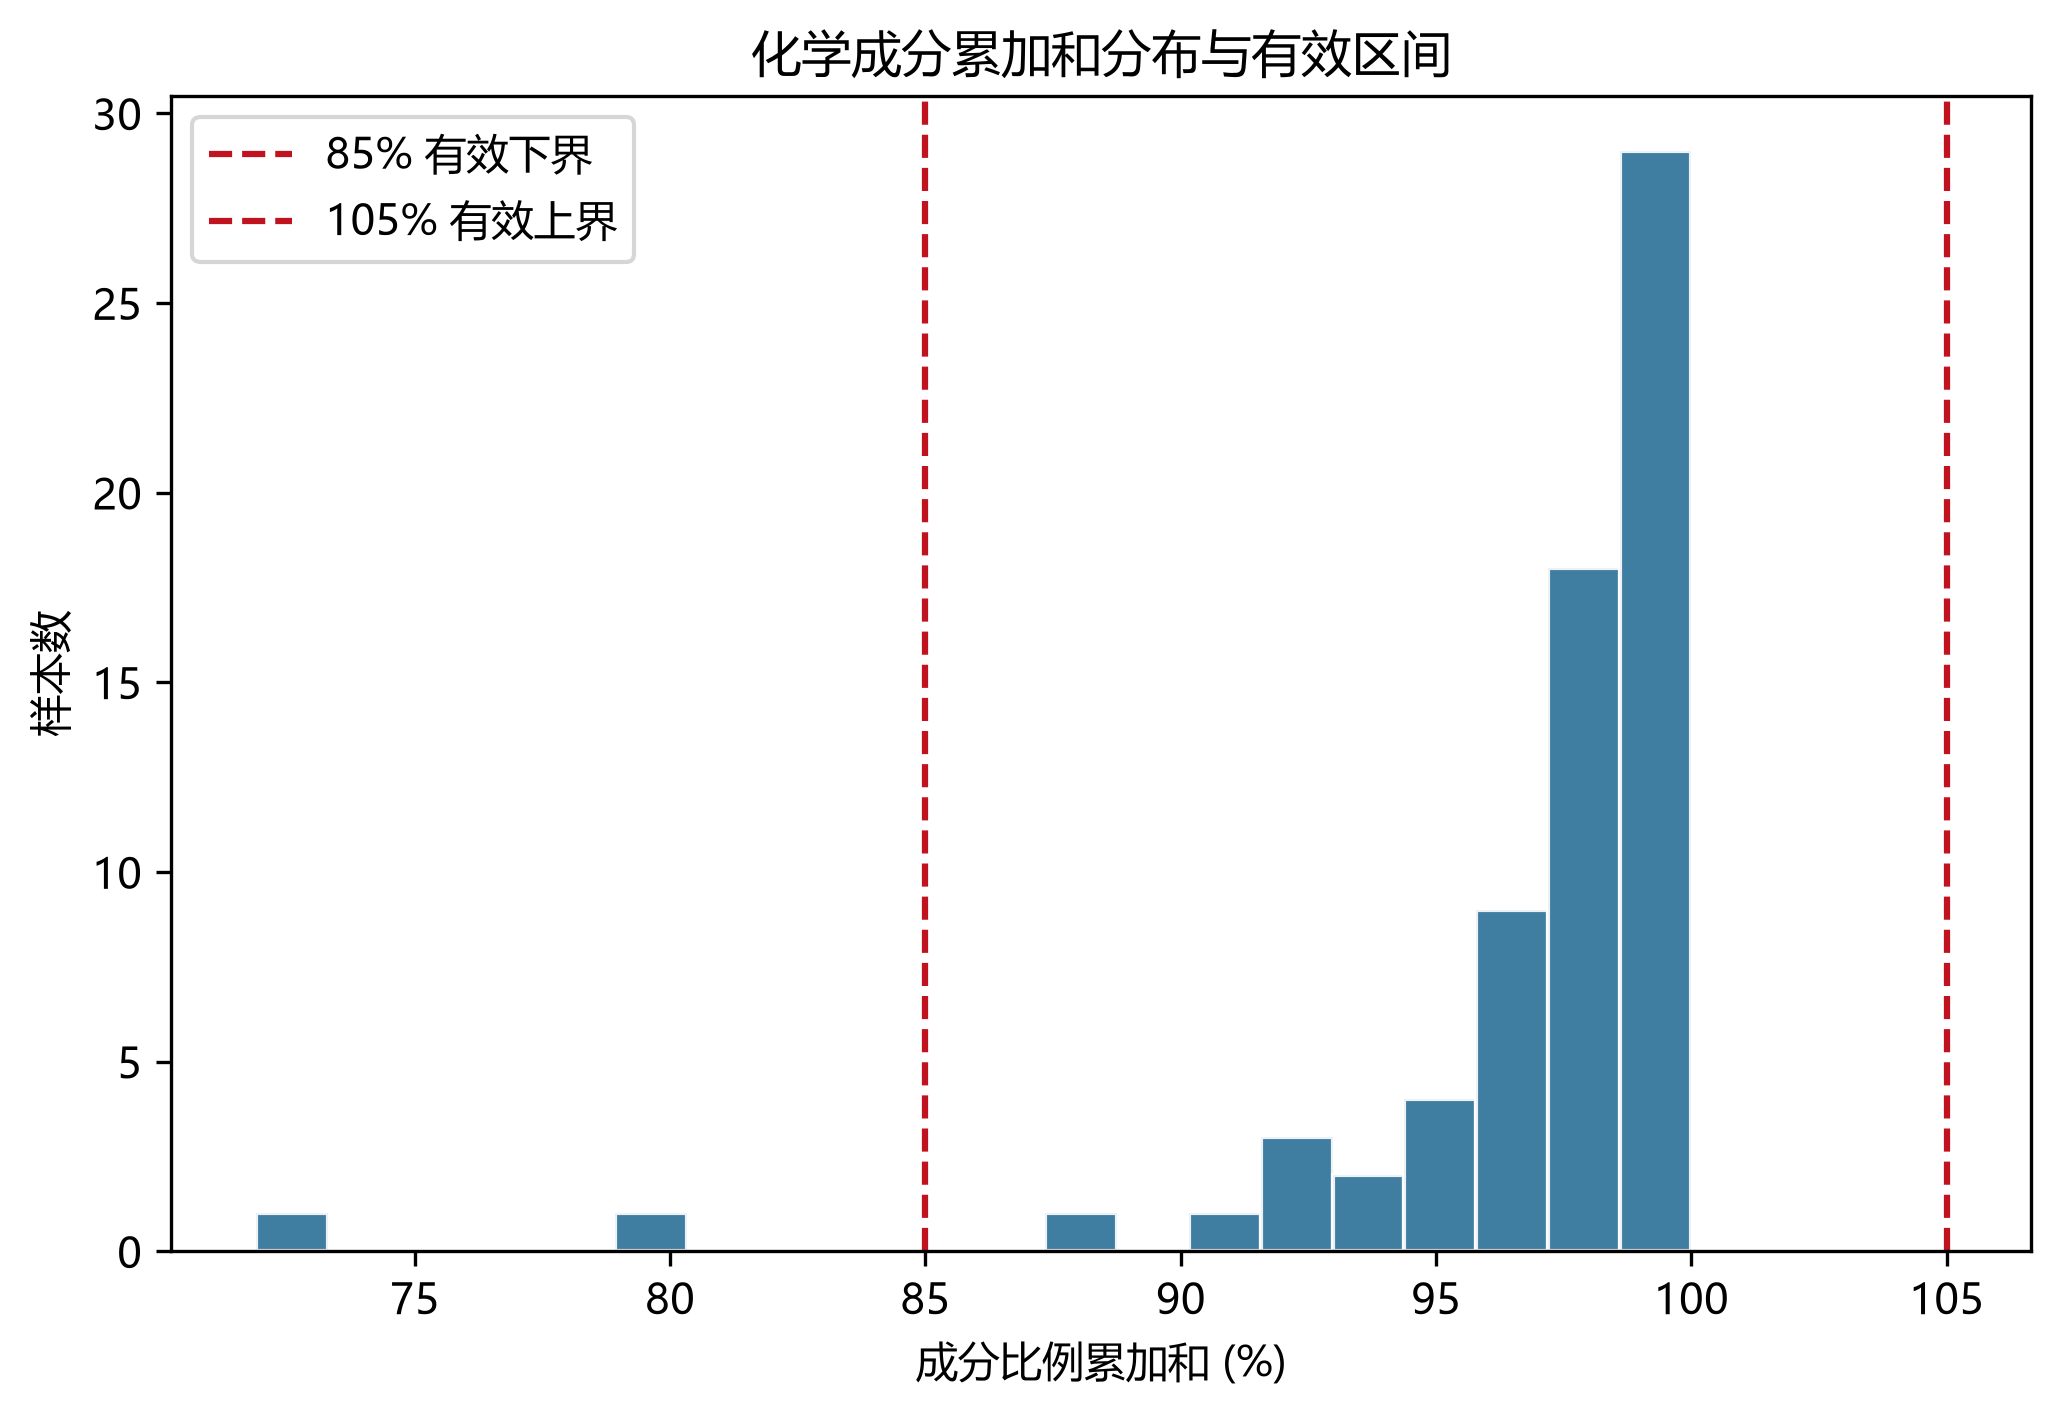
\includegraphics[width=\linewidth]{figures/eda_sum_hist.png}
\caption{成分累加和分布}
\label{fig:sum}
\end{minipage}
\hfill
\begin{minipage}{0.48\textwidth}
\centering
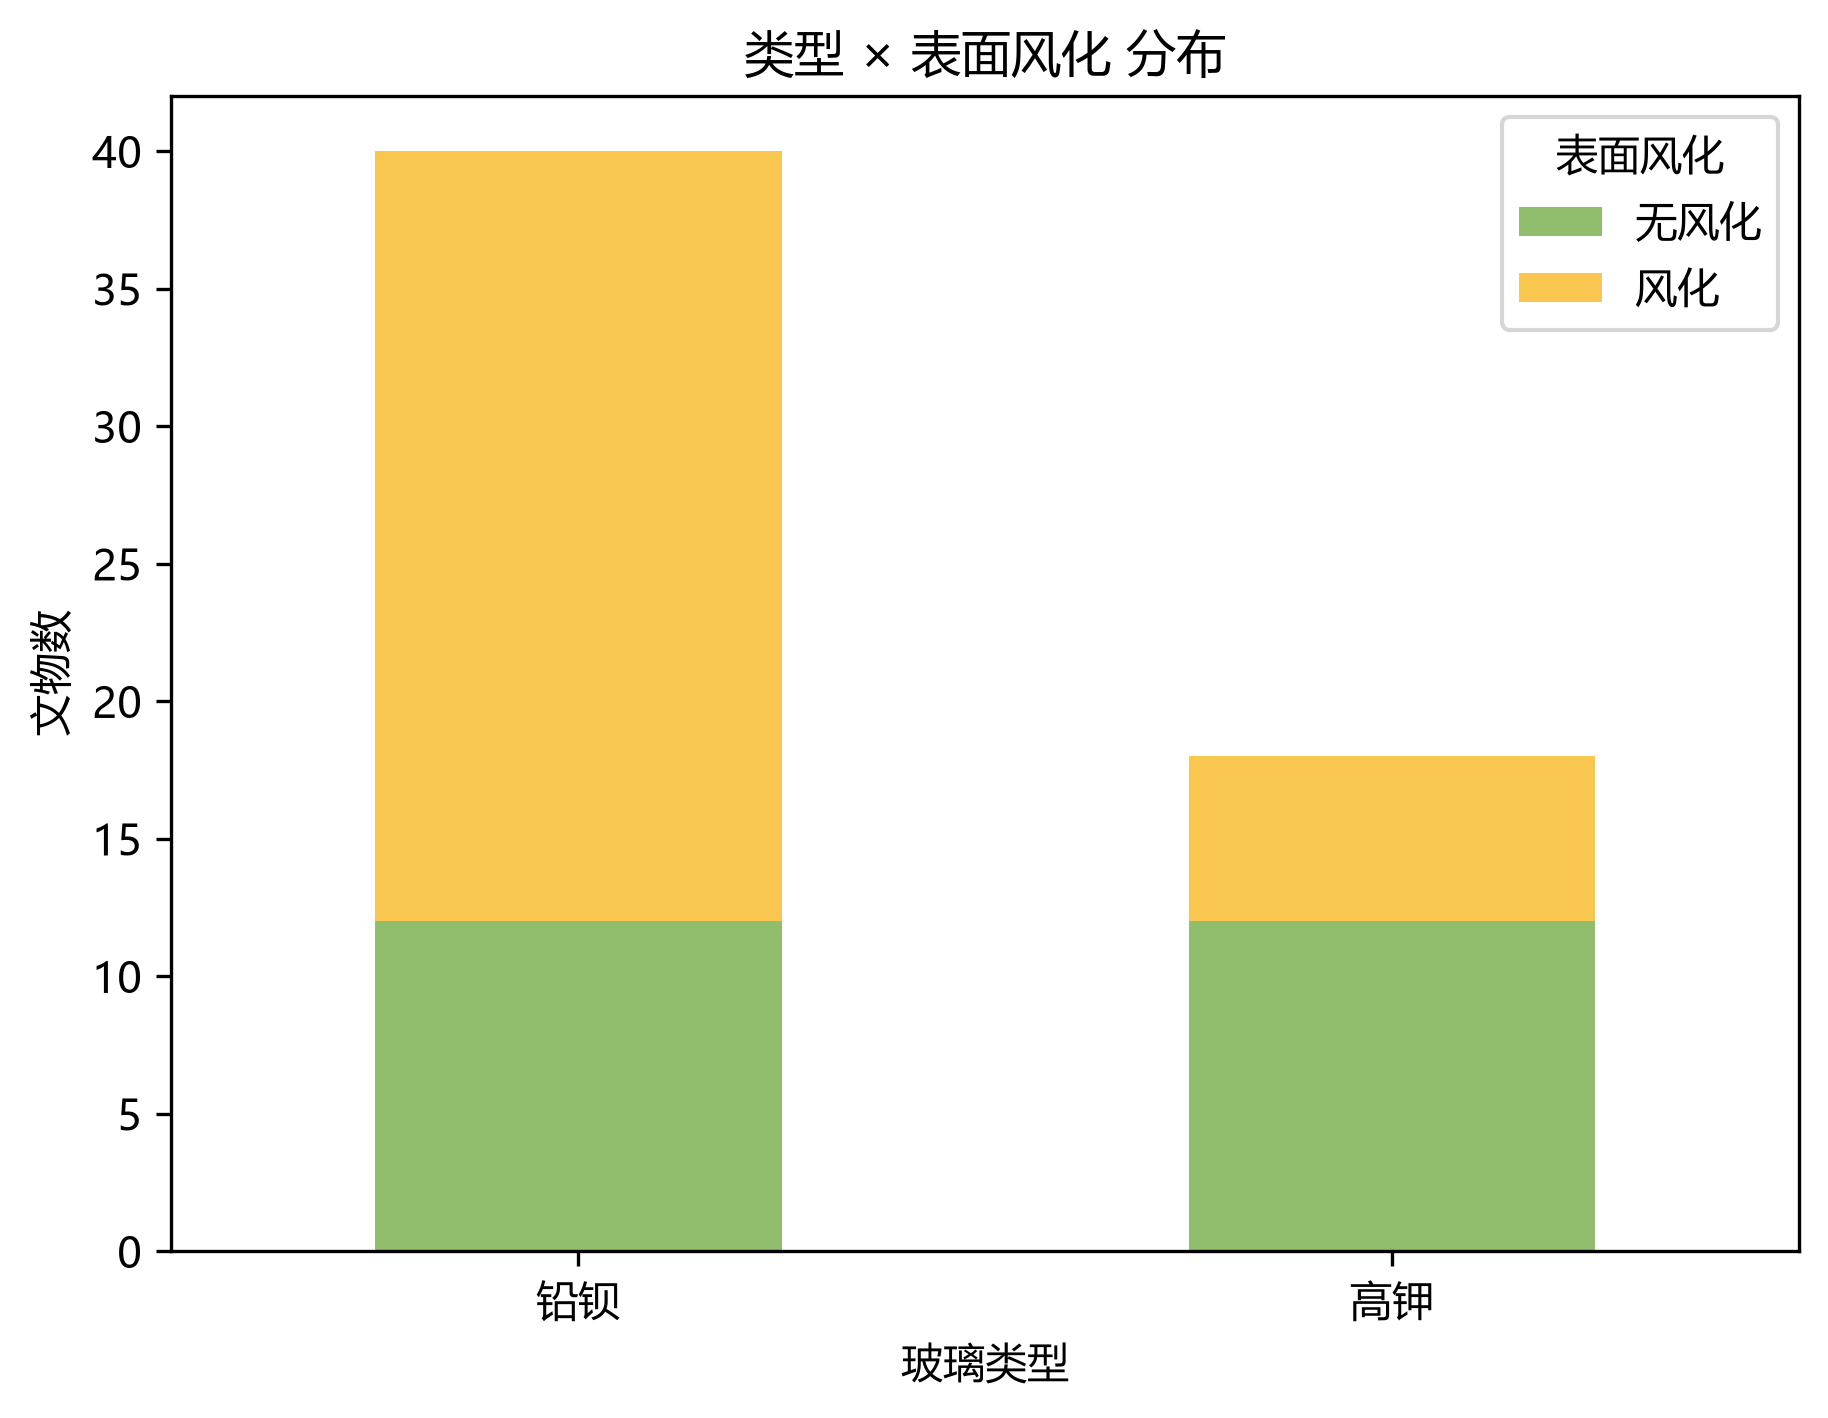
\includegraphics[width=\linewidth]{figures/eda_type_weather_stack.png}
\caption{类型与风化分布}
\label{fig:tw}
\end{minipage}
\end{figure}

\begin{figure}[H]
\centering
\begin{minipage}{0.48\textwidth}
\centering
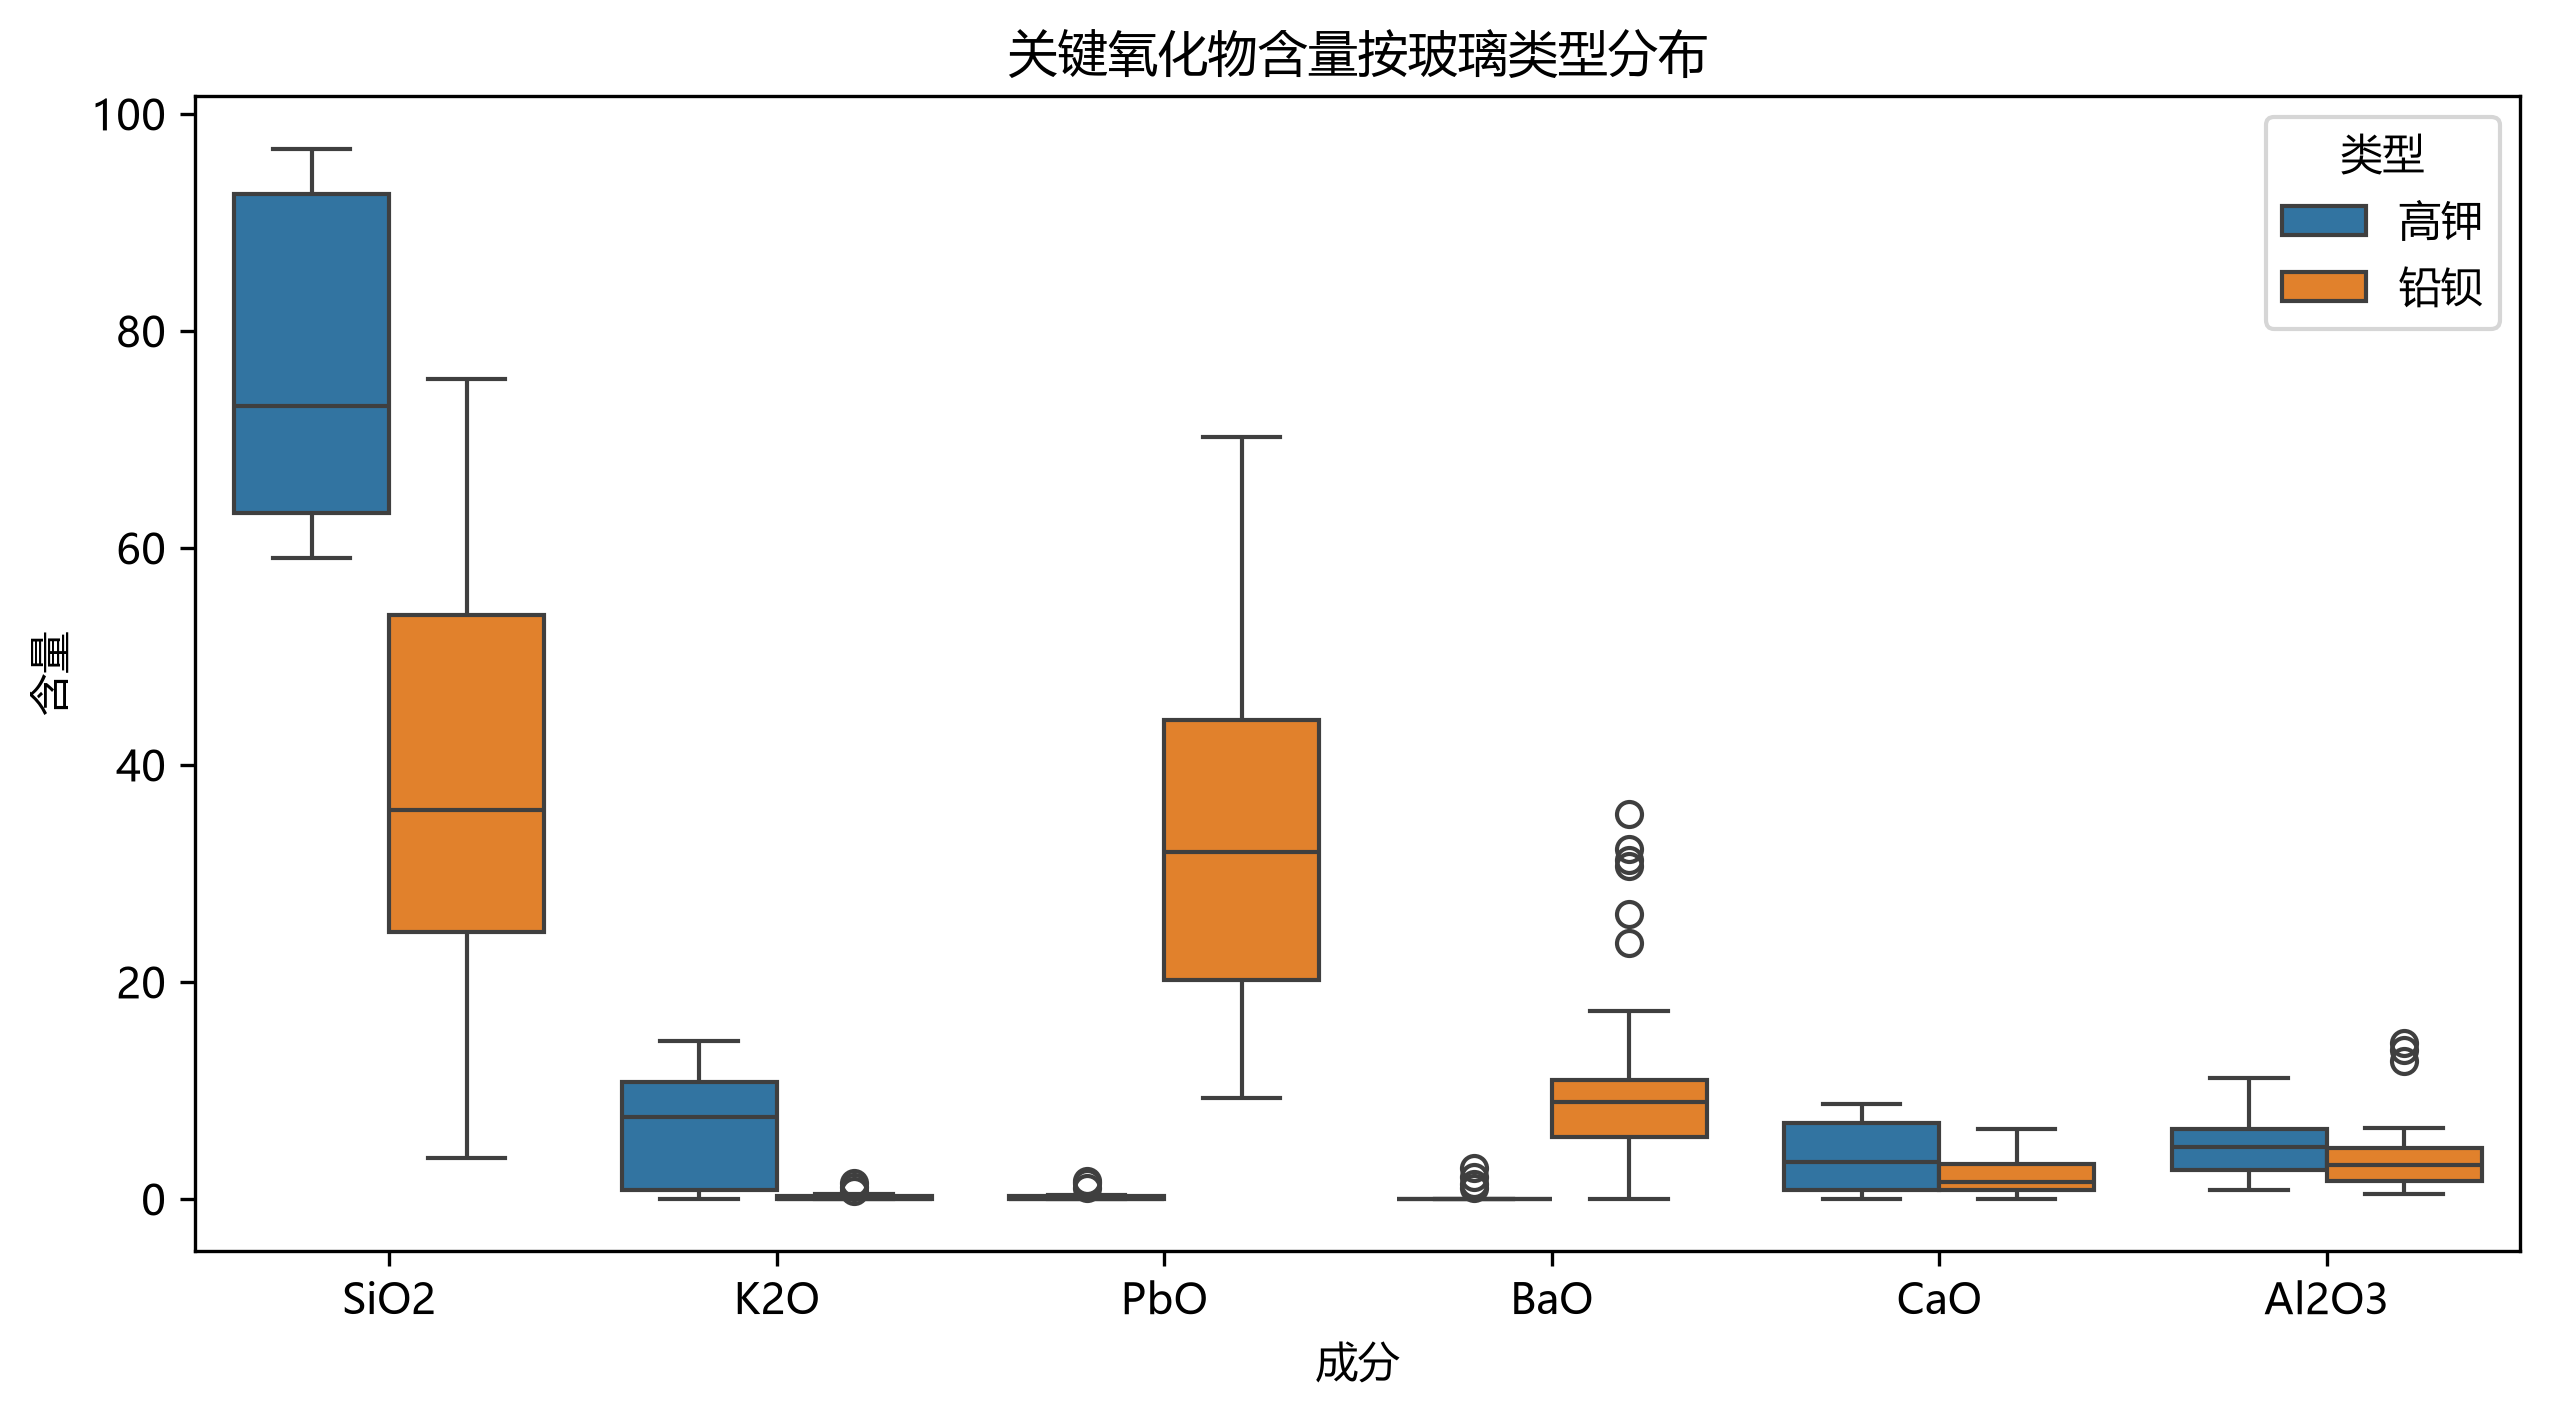
\includegraphics[width=\linewidth]{figures/eda_key_oxides_box.png}
\caption{关键氧化物按类型分布}
\label{fig:box}
\end{minipage}
\hfill
\begin{minipage}{0.48\textwidth}
\centering
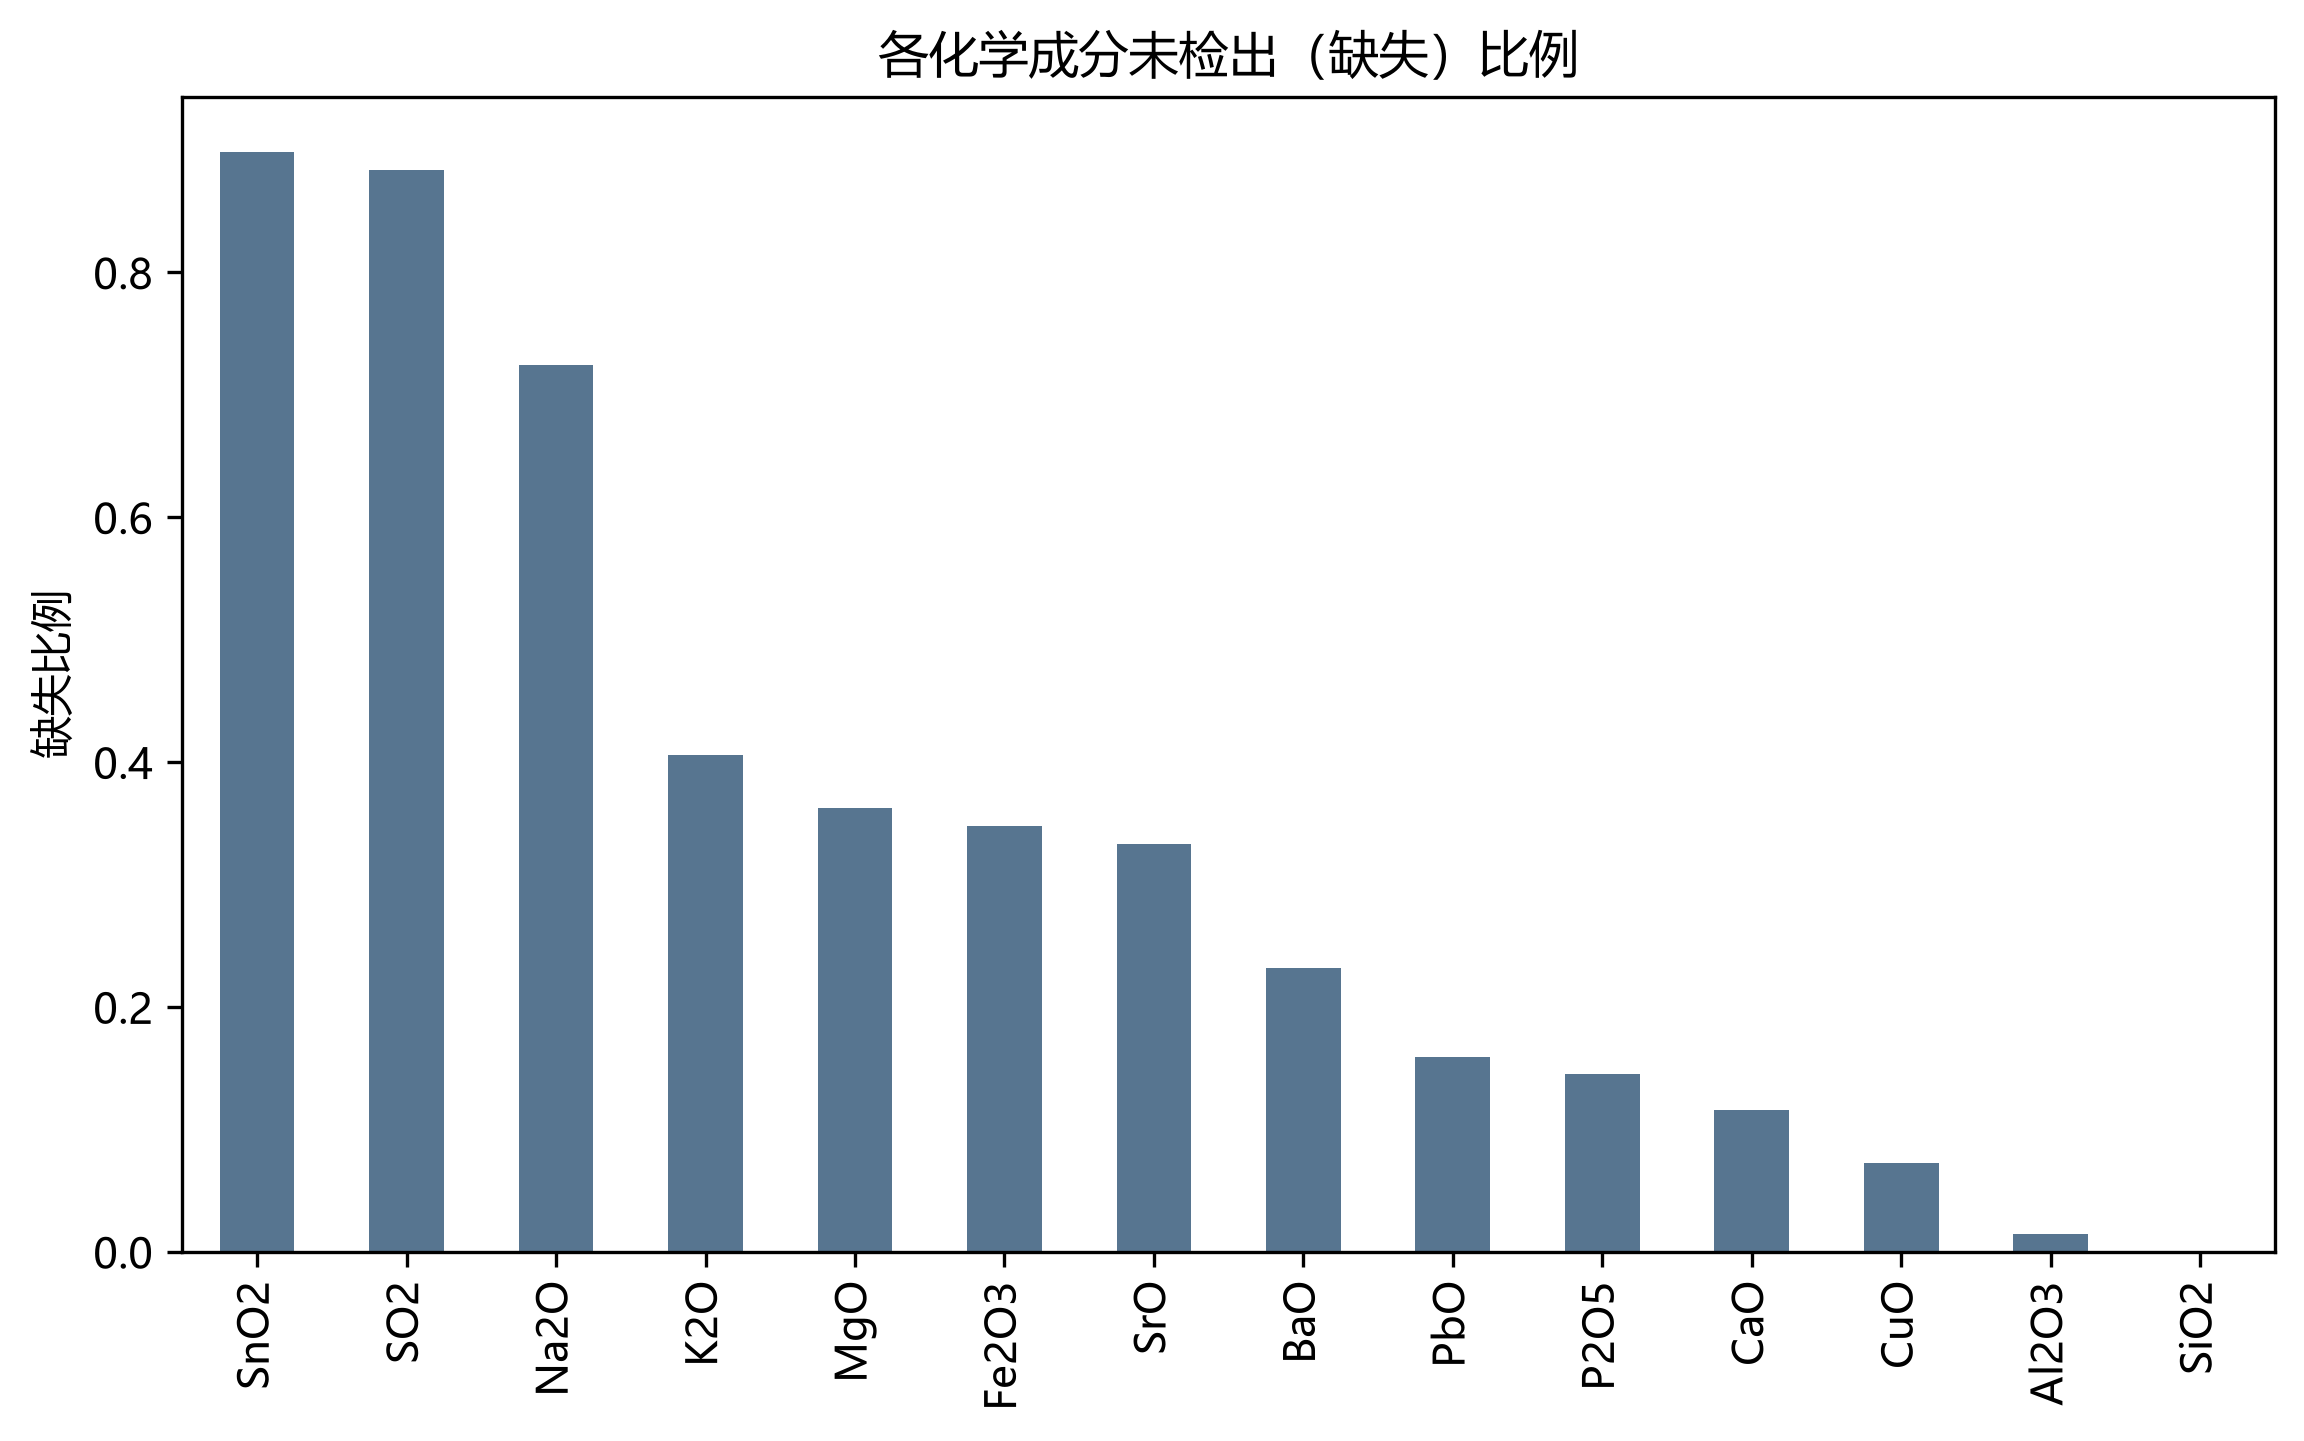
\includegraphics[width=\linewidth]{figures/eda_missing_rate.png}
\caption{各成分未检出比例}
\label{fig:miss}
\end{minipage}
\end{figure}

\begin{figure}[H]
\centering
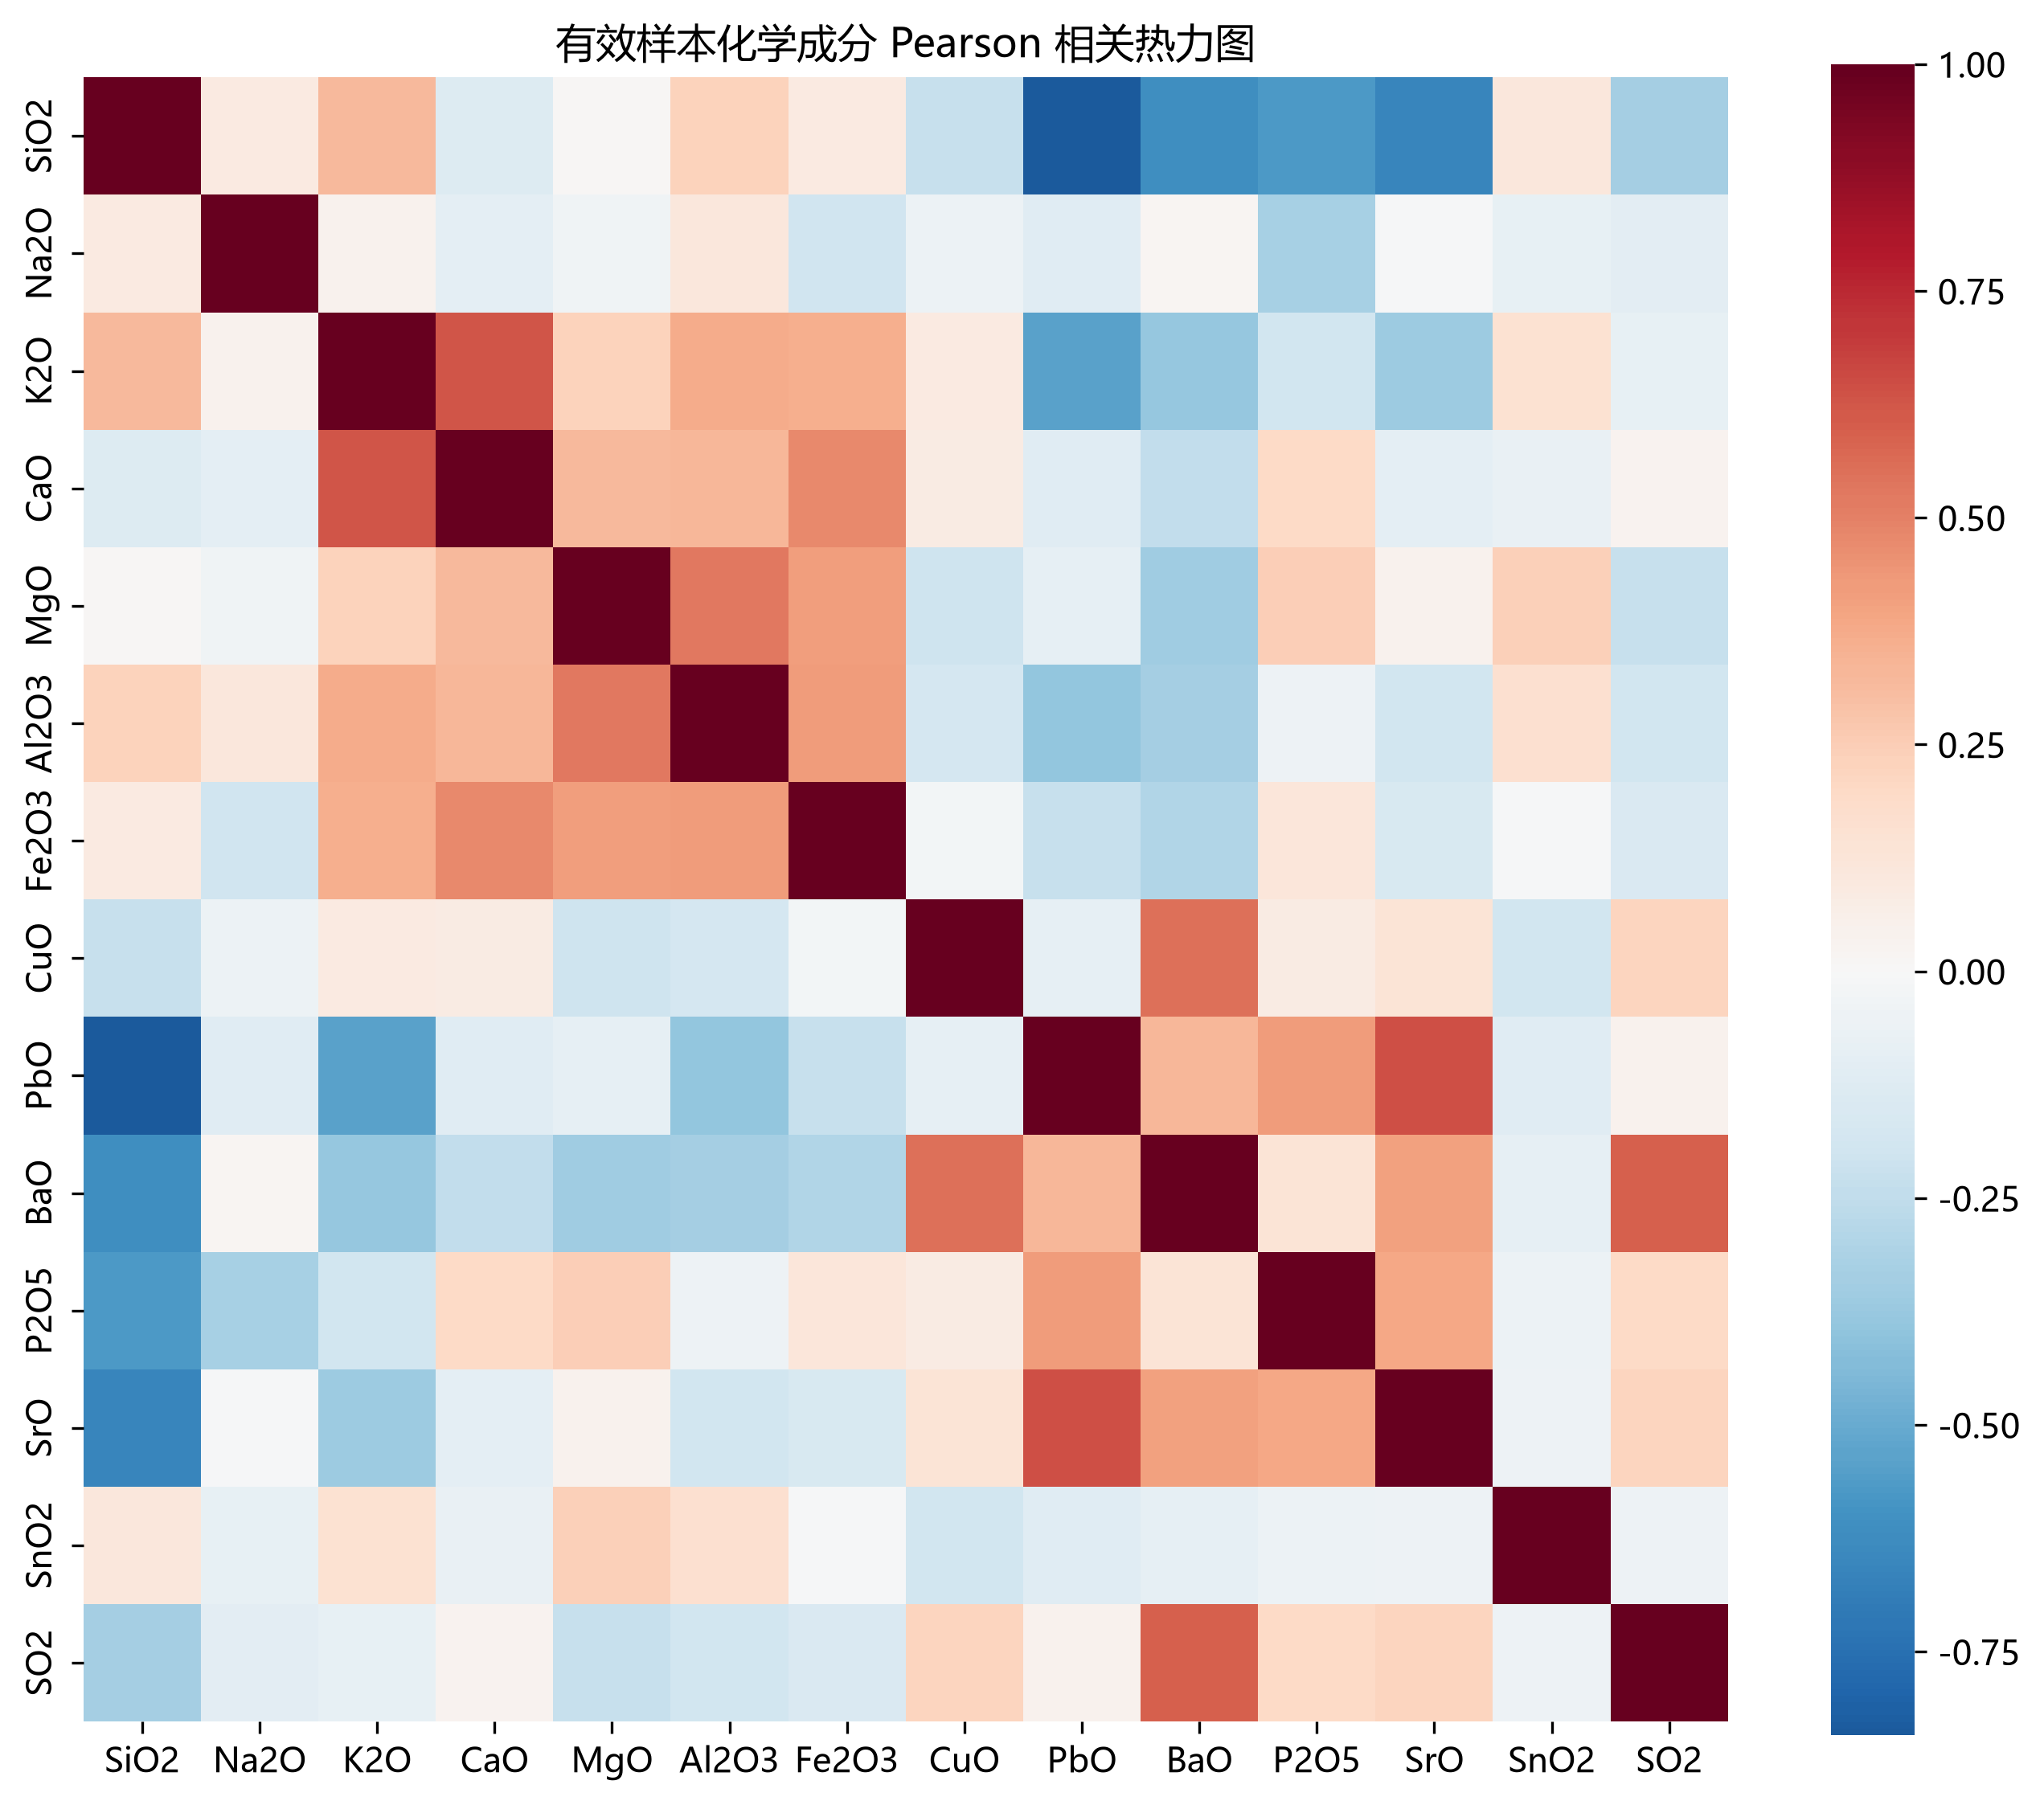
\includegraphics[width=0.82\textwidth]{figures/eda_corr_heatmap.png}
\caption{有效样本成分Pearson相关热力图}
\label{fig:corr}
\end{figure}

纹饰、颜色与风化的交叉分布见图~\ref{fig:decor}--\ref{fig:color}，为问题1关联检验提供直观证据。

\begin{figure}[H]
\centering
\begin{minipage}{0.48\textwidth}
\centering
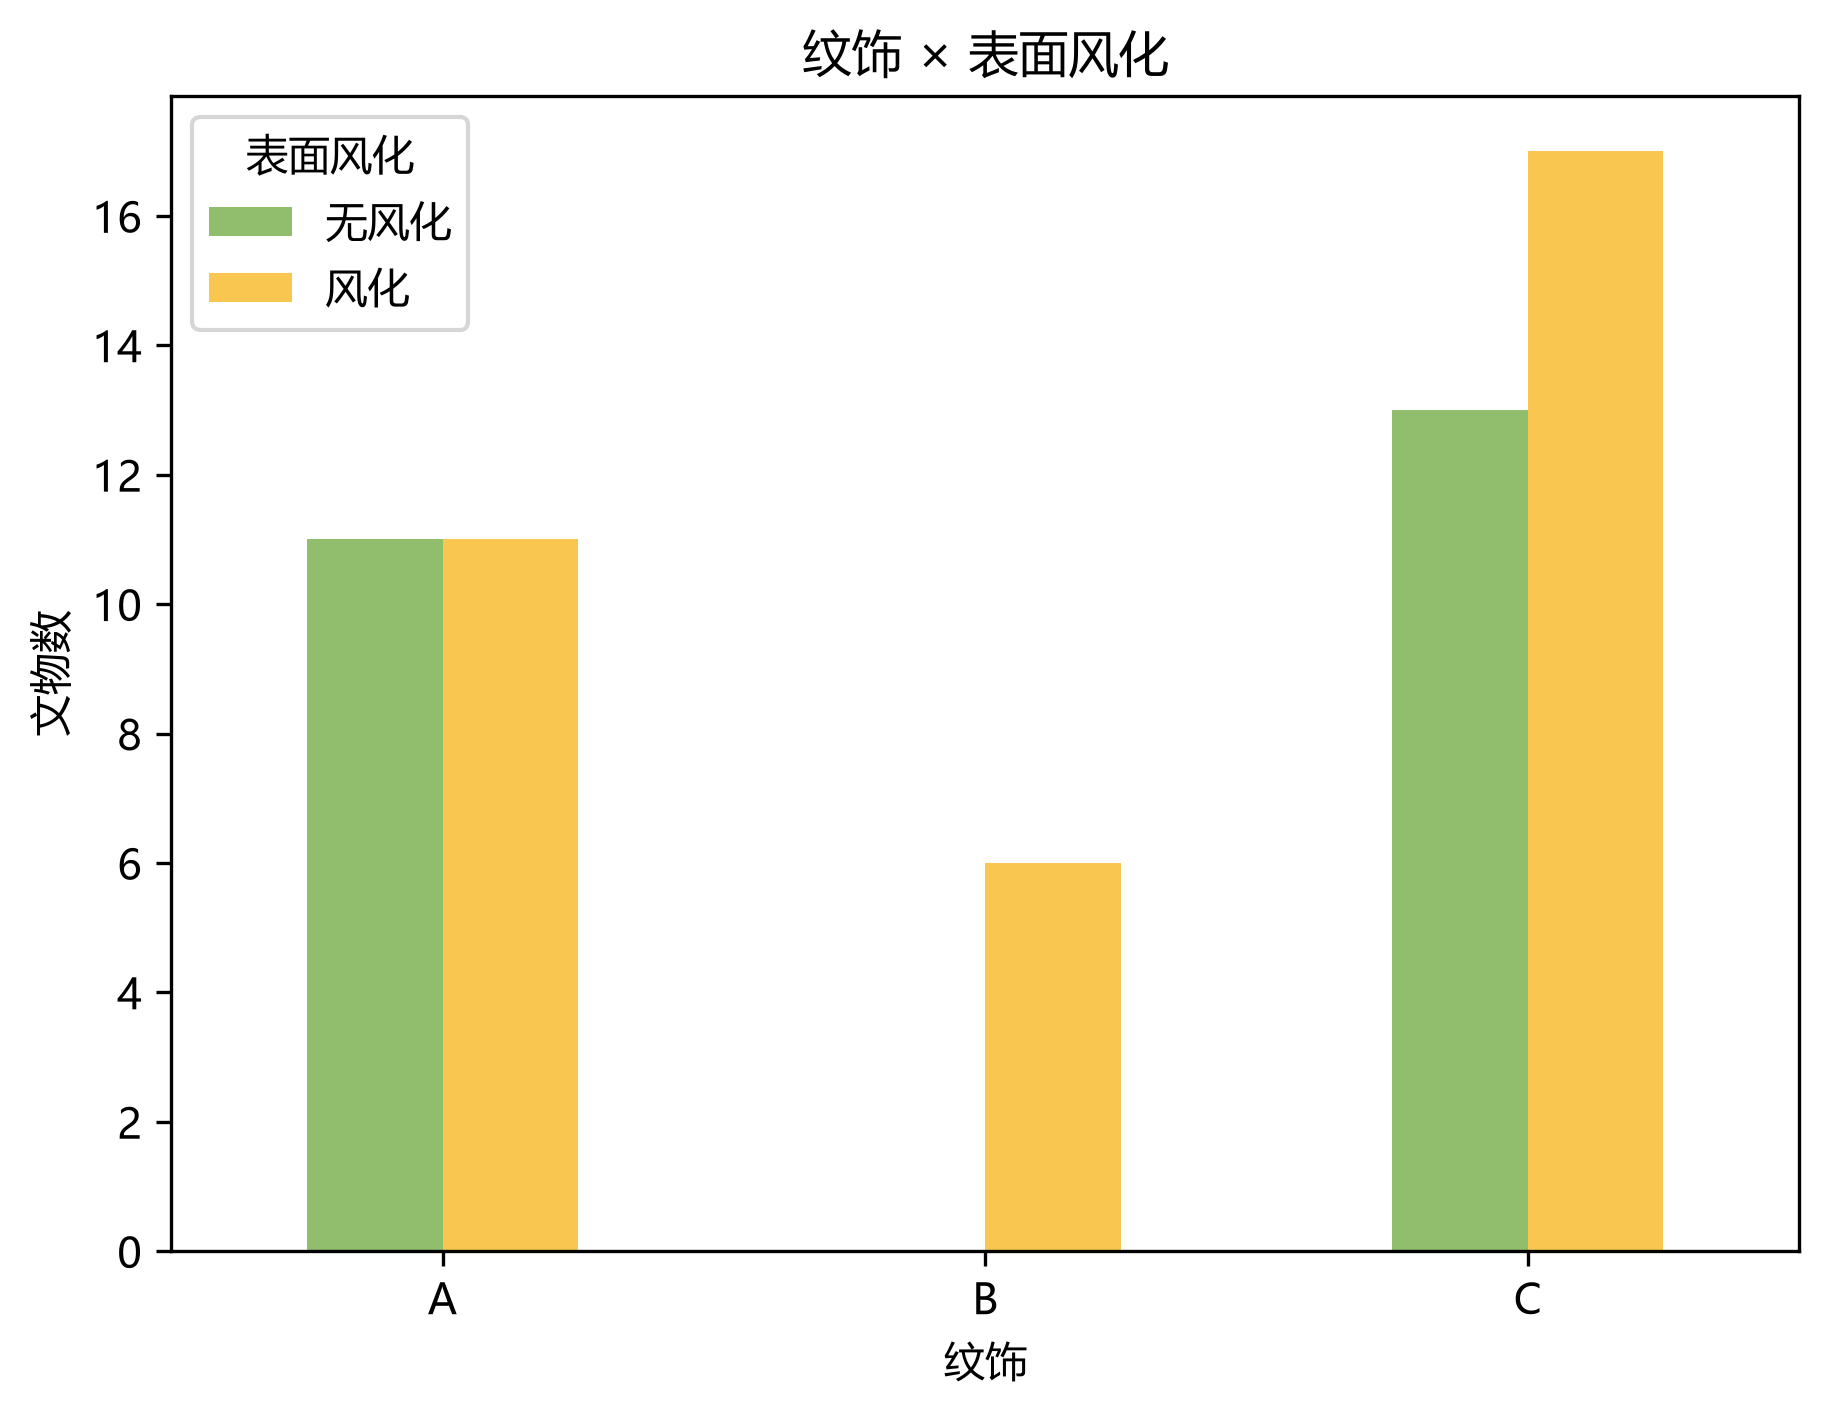
\includegraphics[width=\linewidth]{figures/eda_decor_weather.png}
\caption{纹饰与风化}
\label{fig:decor}
\end{minipage}
\hfill
\begin{minipage}{0.48\textwidth}
\centering
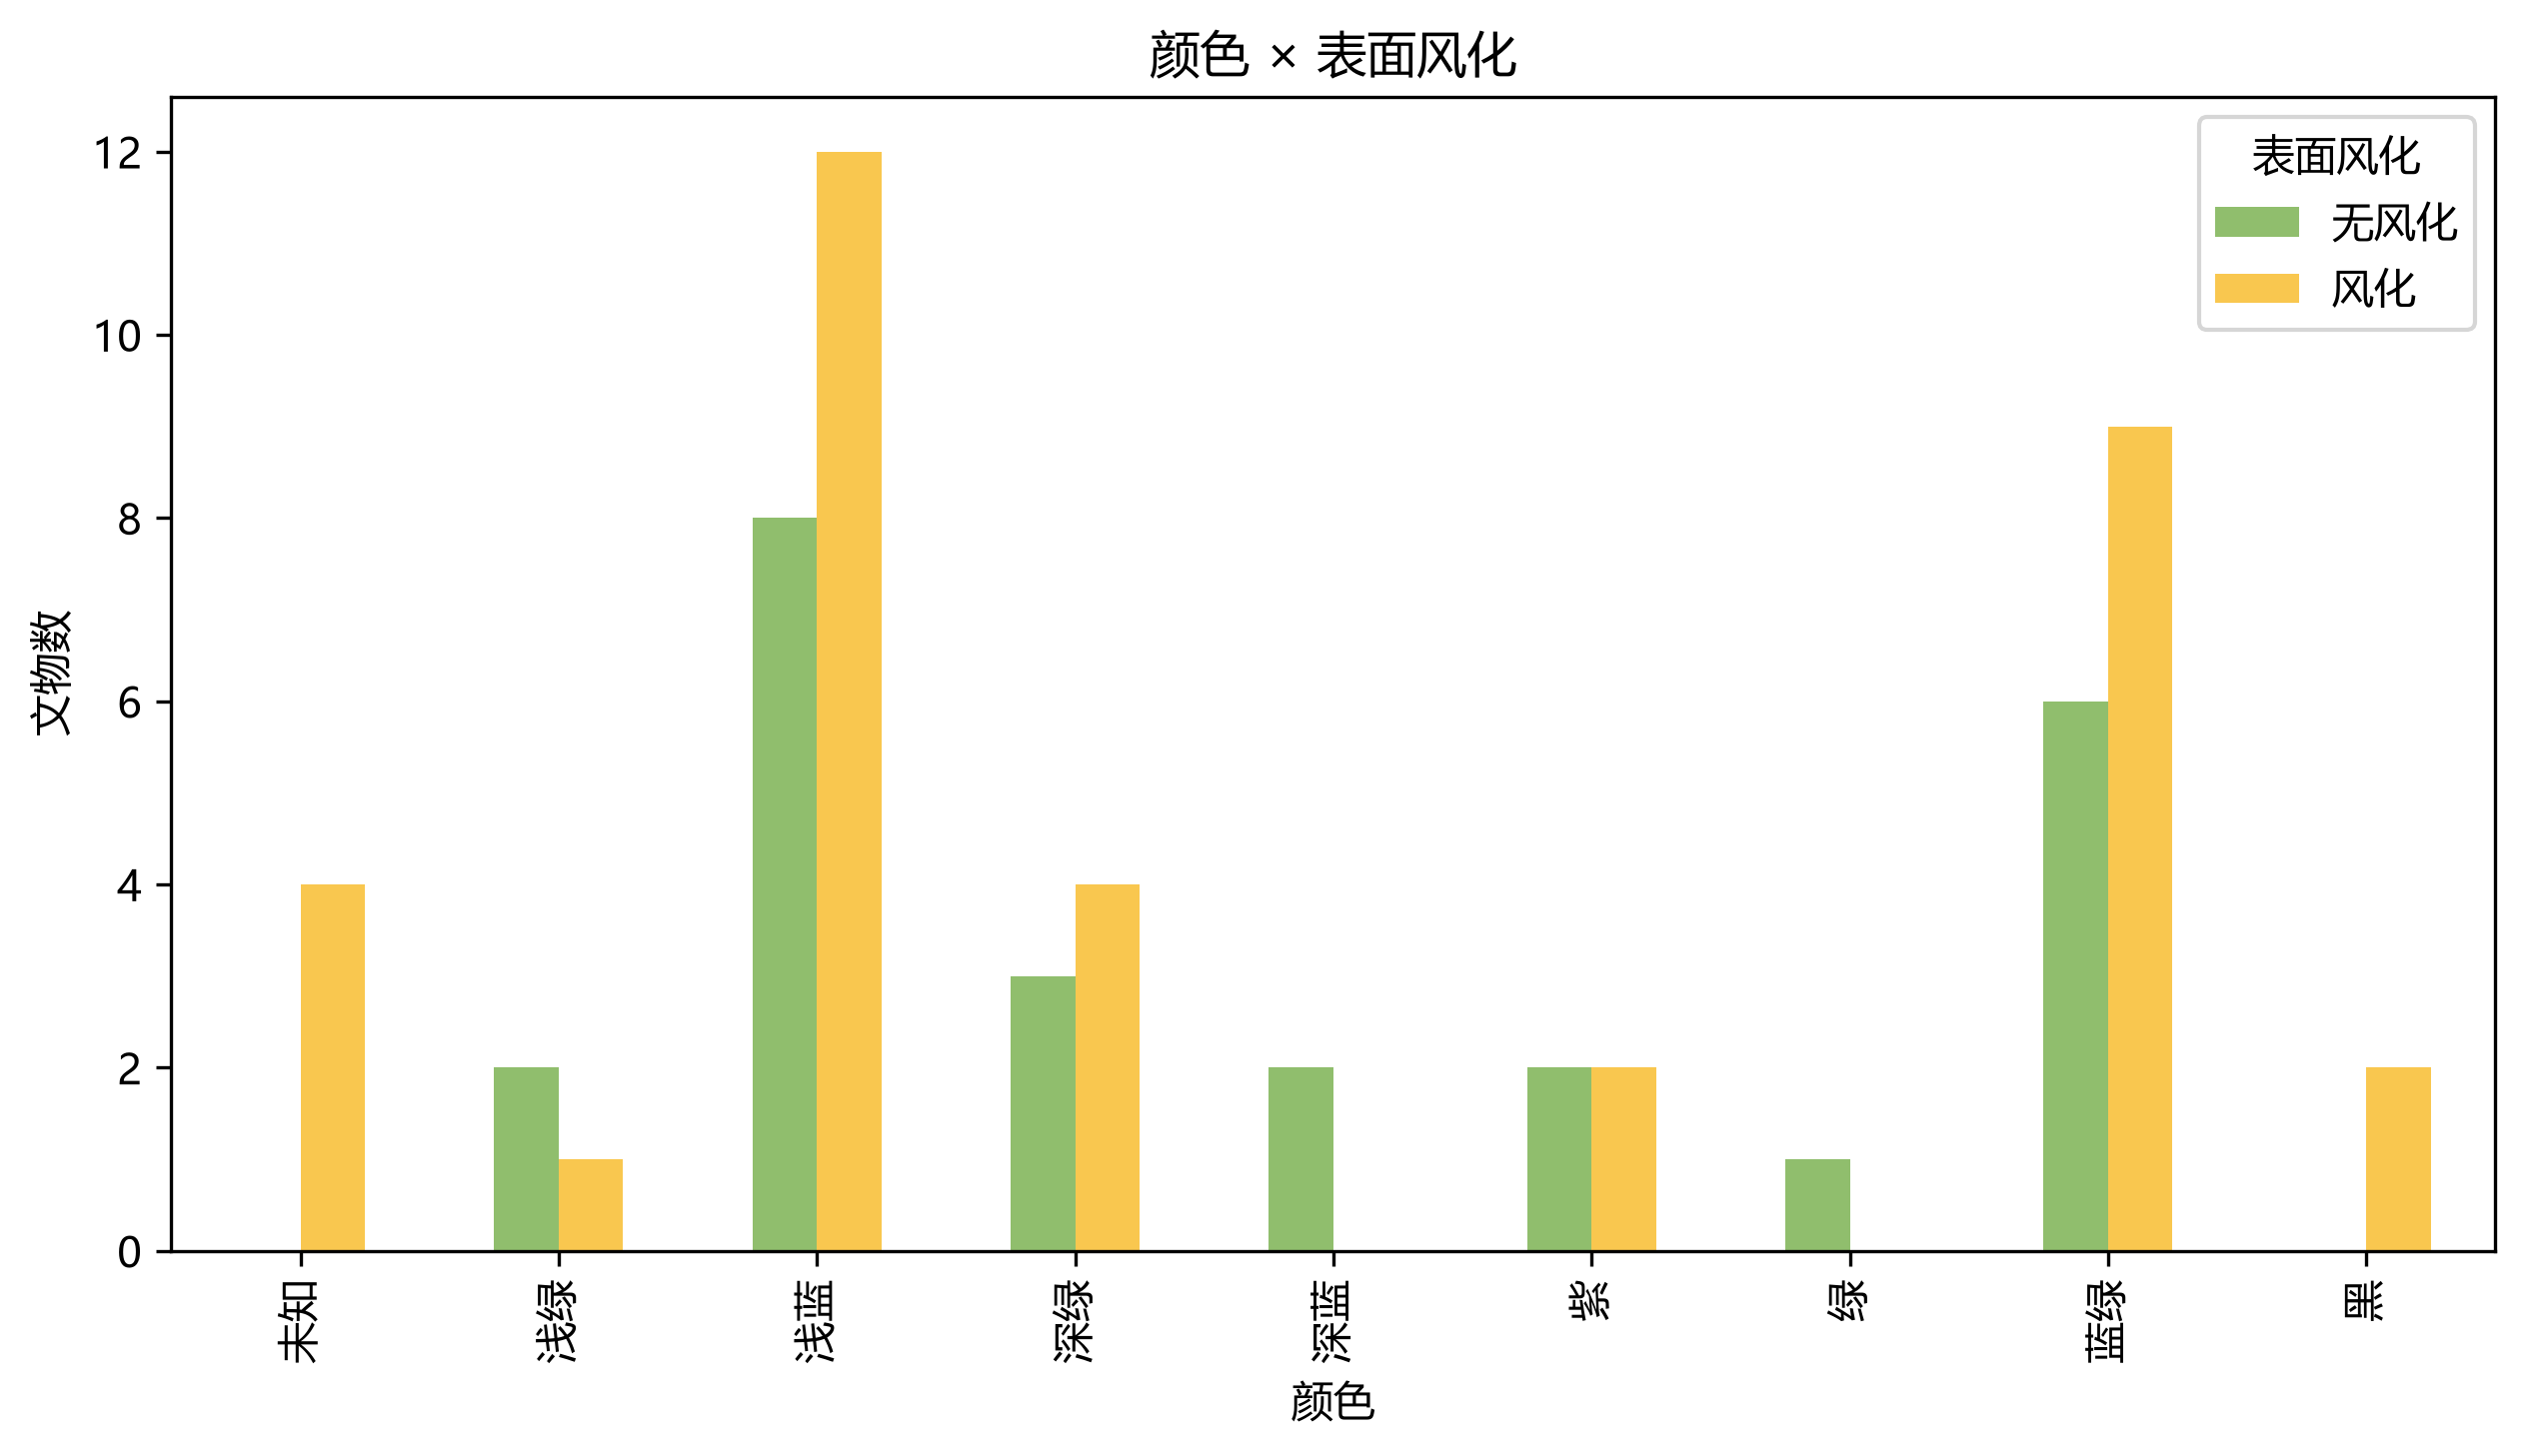
\includegraphics[width=\linewidth]{figures/eda_color_weather.png}
\caption{颜色与风化}
\label{fig:color}
\end{minipage}
\end{figure}

\section{问题1：风化关系、成分规律与风化前预测}
\subsection{问题定位}
Q1要回答两件事：哪些属性与风化相关；风化如何改变成分，以及如何由风化点回推风化前成分。其输出为后续分类提供“观测被扭曲”的机制解释。

\subsection{关联分析模型}
对属性$A\in\{\text{类型},\text{纹饰},\text{颜色}\}$与风化$W$，构造列联表并计算
\begin{equation}
\chi^2=\sum_{u,v}\frac{(O_{uv}-E_{uv})^2}{E_{uv}},\qquad
V=\sqrt{\frac{\chi^2/n}{\min(r-1,k-1)}},
\end{equation}
其中$V$为Cramer's $V$。对$2\times2$且样本量偏小时改用Fisher精确检验。结果见表~\ref{tab:assoc}与图~\ref{fig:q1ct}。

\begin{table}[H]
\centering
\caption{风化与类型/纹饰/颜色的关联检验}
\label{tab:assoc}
\scriptsize
\begin{tabular}{lccccc}
\toprule
变量 & 检验 & 统计量 & p值 & CramersV & 显著 \\
\hline
类型 & Chi2 & 5.452 & 0.020 & 0.344 & 是 \\
纹饰 & Chi2 & 4.957 & 0.084 & 0.292 & 否 \\
颜色 & Chi2 & 9.432 & 0.307 & 0.403 & 否 \\
\bottomrule
\end{tabular}
\end{table}

\begin{figure}[H]
\centering
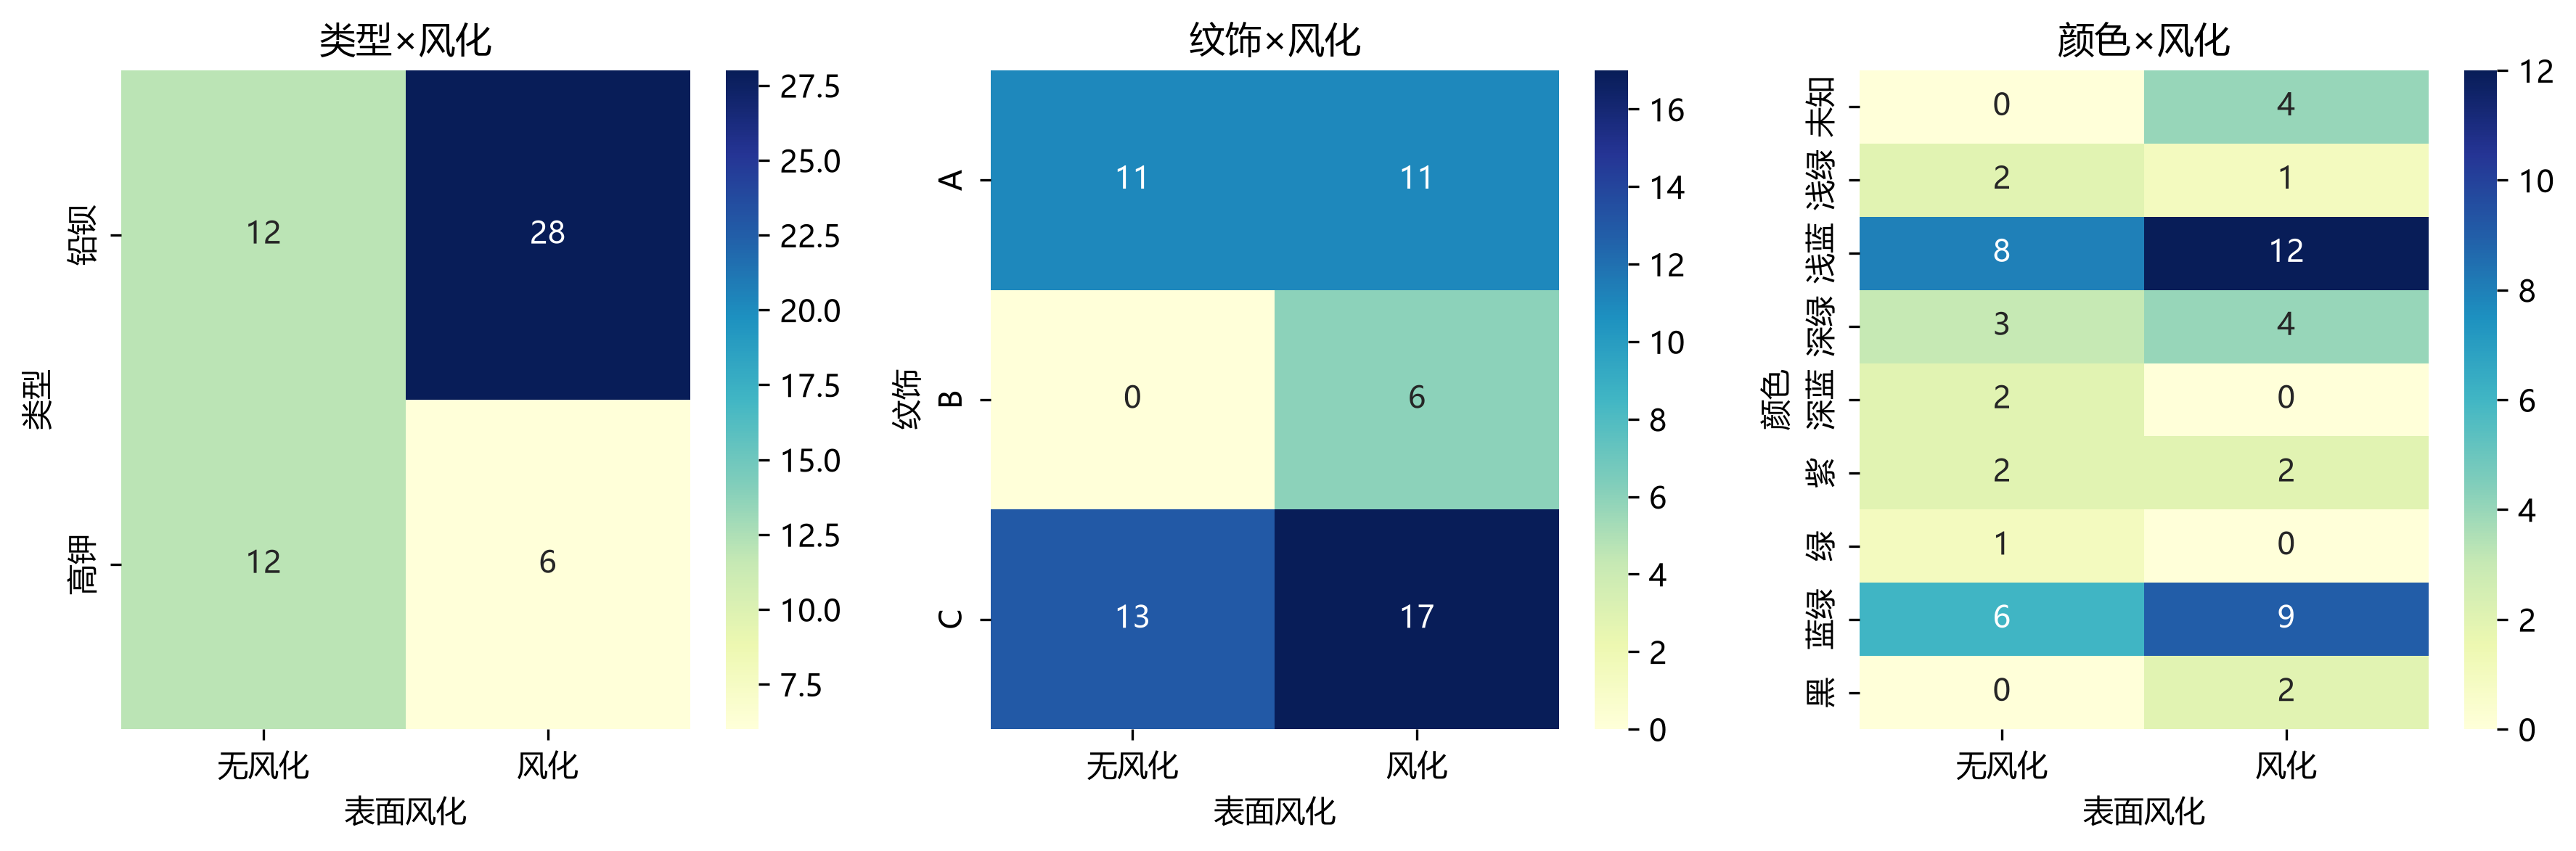
\includegraphics[width=0.95\textwidth]{figures/q1_crosstab_heatmaps.png}
\caption{列联表热力图}
\label{fig:q1ct}
\end{figure}

经验风化率：高钾33.33\%，铅钡70.00\%，铅钡显著更易被标记为表面风化。

\subsection{类型分层的成分统计规律}
对固定类型$t$，比较风化与无风化两组成分。由于小样本且偏态常见，采用Mann-Whitney $U$检验：
\begin{equation}
U=n_1 n_2+\frac{n_1(n_1+1)}{2}-R_1,
\end{equation}
并报告均值差$\Delta_c=\bar{x}_c^{\text{风化}}-\bar{x}_c^{\text{无风化}}$。显著成分数共15个，部分结果见表~\ref{tab:mw}与图~\ref{fig:q1diff}。

\begin{table}[H]
\centering
\caption{风化与无风化成分差异（显著或代表性结果）}
\label{tab:mw}
\scriptsize
\begin{tabular}{lccccc}
\toprule
类型 & 成分 & 风化均值 & 无风化均值 & 差值 & p值 \\
\hline
高钾 & SiO2 & 93.963 & 67.984 & 25.979 & 0.000 \\
高钾 & K2O & 0.543 & 9.331 & -8.787 & 0.004 \\
高钾 & CaO & 0.870 & 5.333 & -4.463 & 0.028 \\
高钾 & MgO & 0.197 & 1.079 & -0.882 & 0.015 \\
高钾 & Al2O3 & 1.930 & 6.620 & -4.690 & 0.000 \\
高钾 & Fe2O3 & 0.265 & 1.932 & -1.667 & 0.028 \\
高钾 & PbO & 0.000 & 0.412 & -0.412 & 0.029 \\
高钾 & P2O5 & 0.280 & 1.403 & -1.122 & 0.015 \\
铅钡 & SiO2 & 24.913 & 54.660 & -29.747 & 0.000 \\
铅钡 & Na2O & 0.216 & 1.683 & -1.466 & 0.012 \\
铅钡 & CaO & 2.695 & 1.320 & 1.375 & 0.002 \\
铅钡 & Al2O3 & 2.970 & 4.456 & -1.486 & 0.024 \\
铅钡 & PbO & 43.314 & 22.085 & 21.229 & 0.000 \\
铅钡 & P2O5 & 5.277 & 1.049 & 4.228 & 0.000 \\
铅钡 & SrO & 0.418 & 0.268 & 0.150 & 0.032 \\
\bottomrule
\end{tabular}
\end{table}

\begin{figure}[H]
\centering
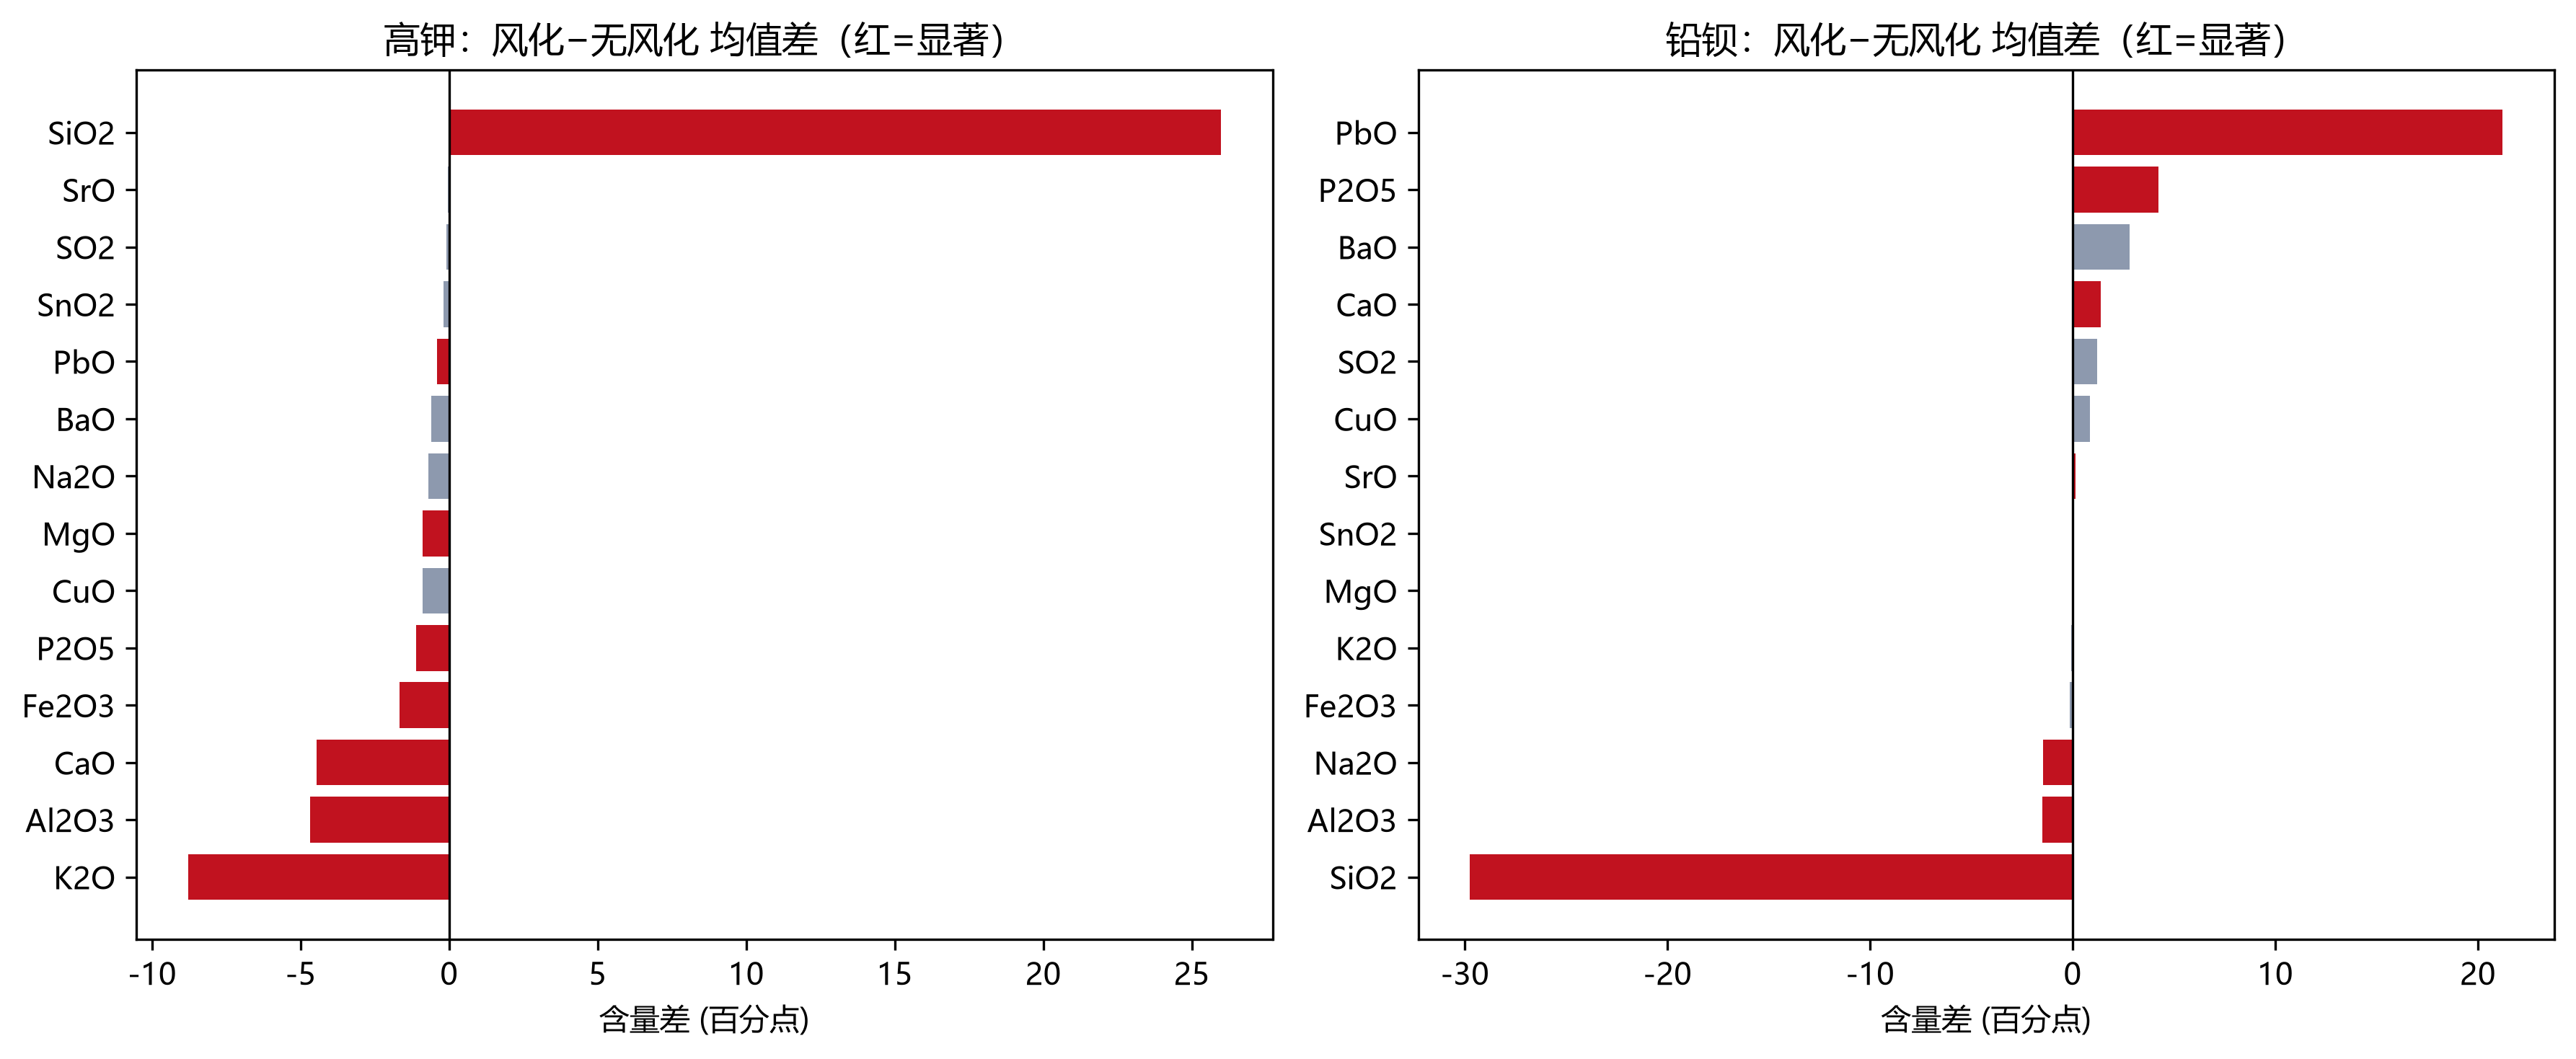
\includegraphics[width=0.95\textwidth]{figures/q1_weather_diff_components.png}
\caption{各成分风化减无风化均值差}
\label{fig:q1diff}
\end{figure}

\begin{figure}[H]
\centering
\begin{minipage}{0.48\textwidth}
\centering
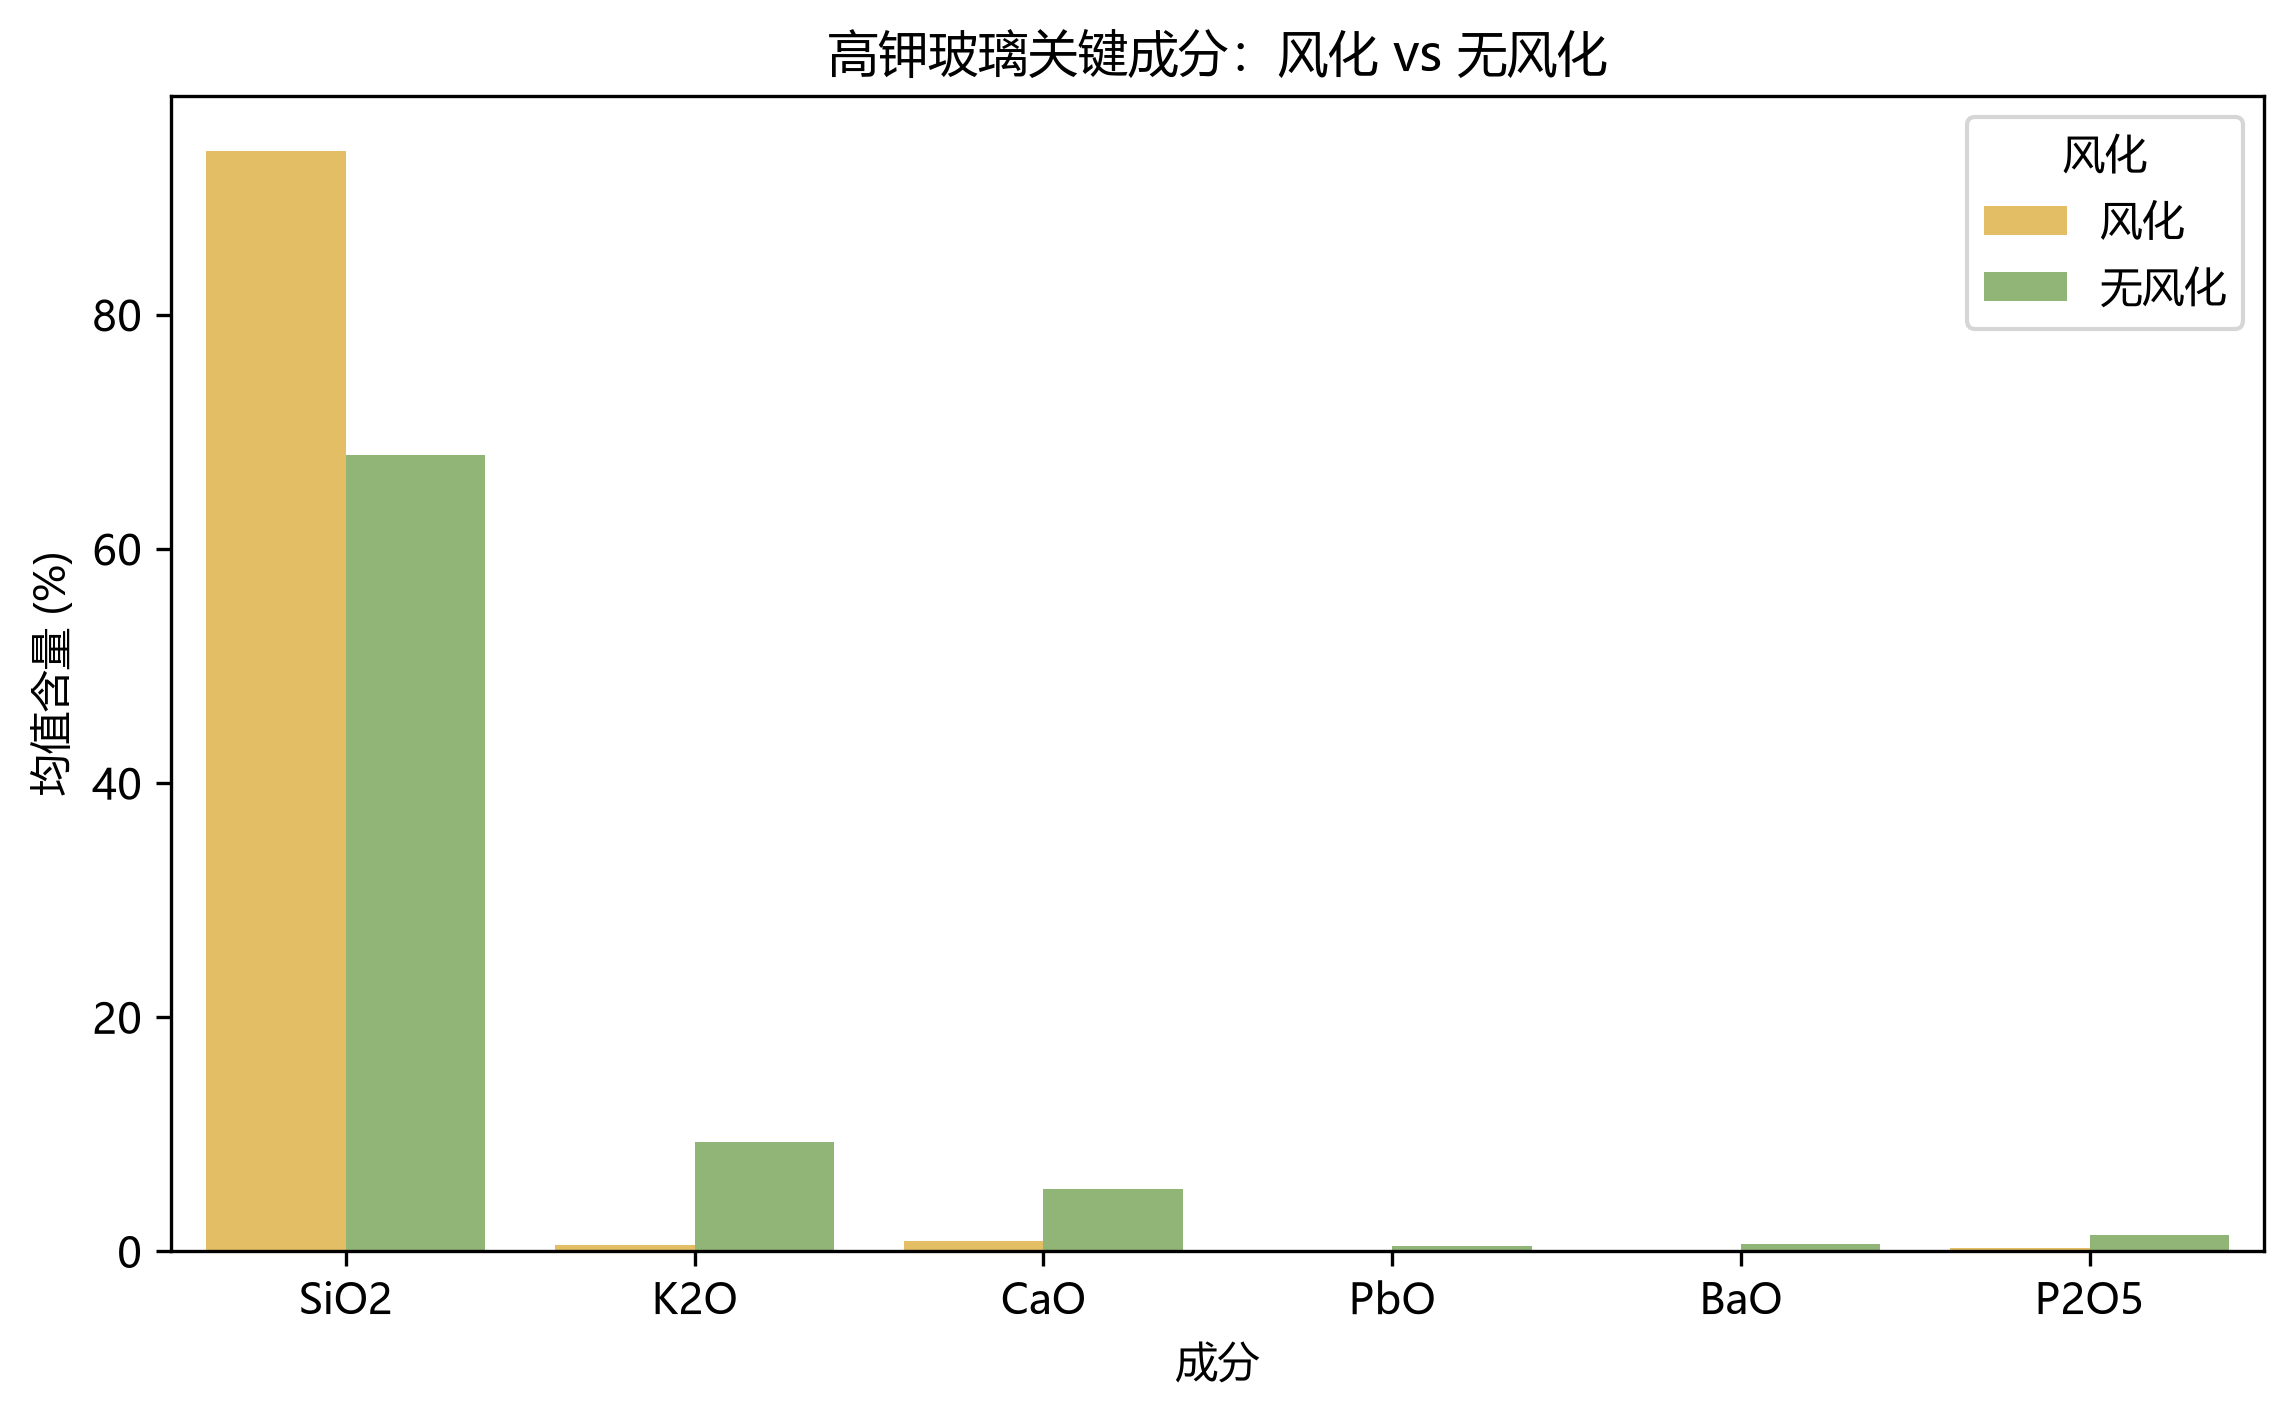
\includegraphics[width=\linewidth]{figures/q1_高钾_weather_bars.png}
\caption{高钾关键成分对比}
\label{fig:hkbar}
\end{minipage}
\hfill
\begin{minipage}{0.48\textwidth}
\centering
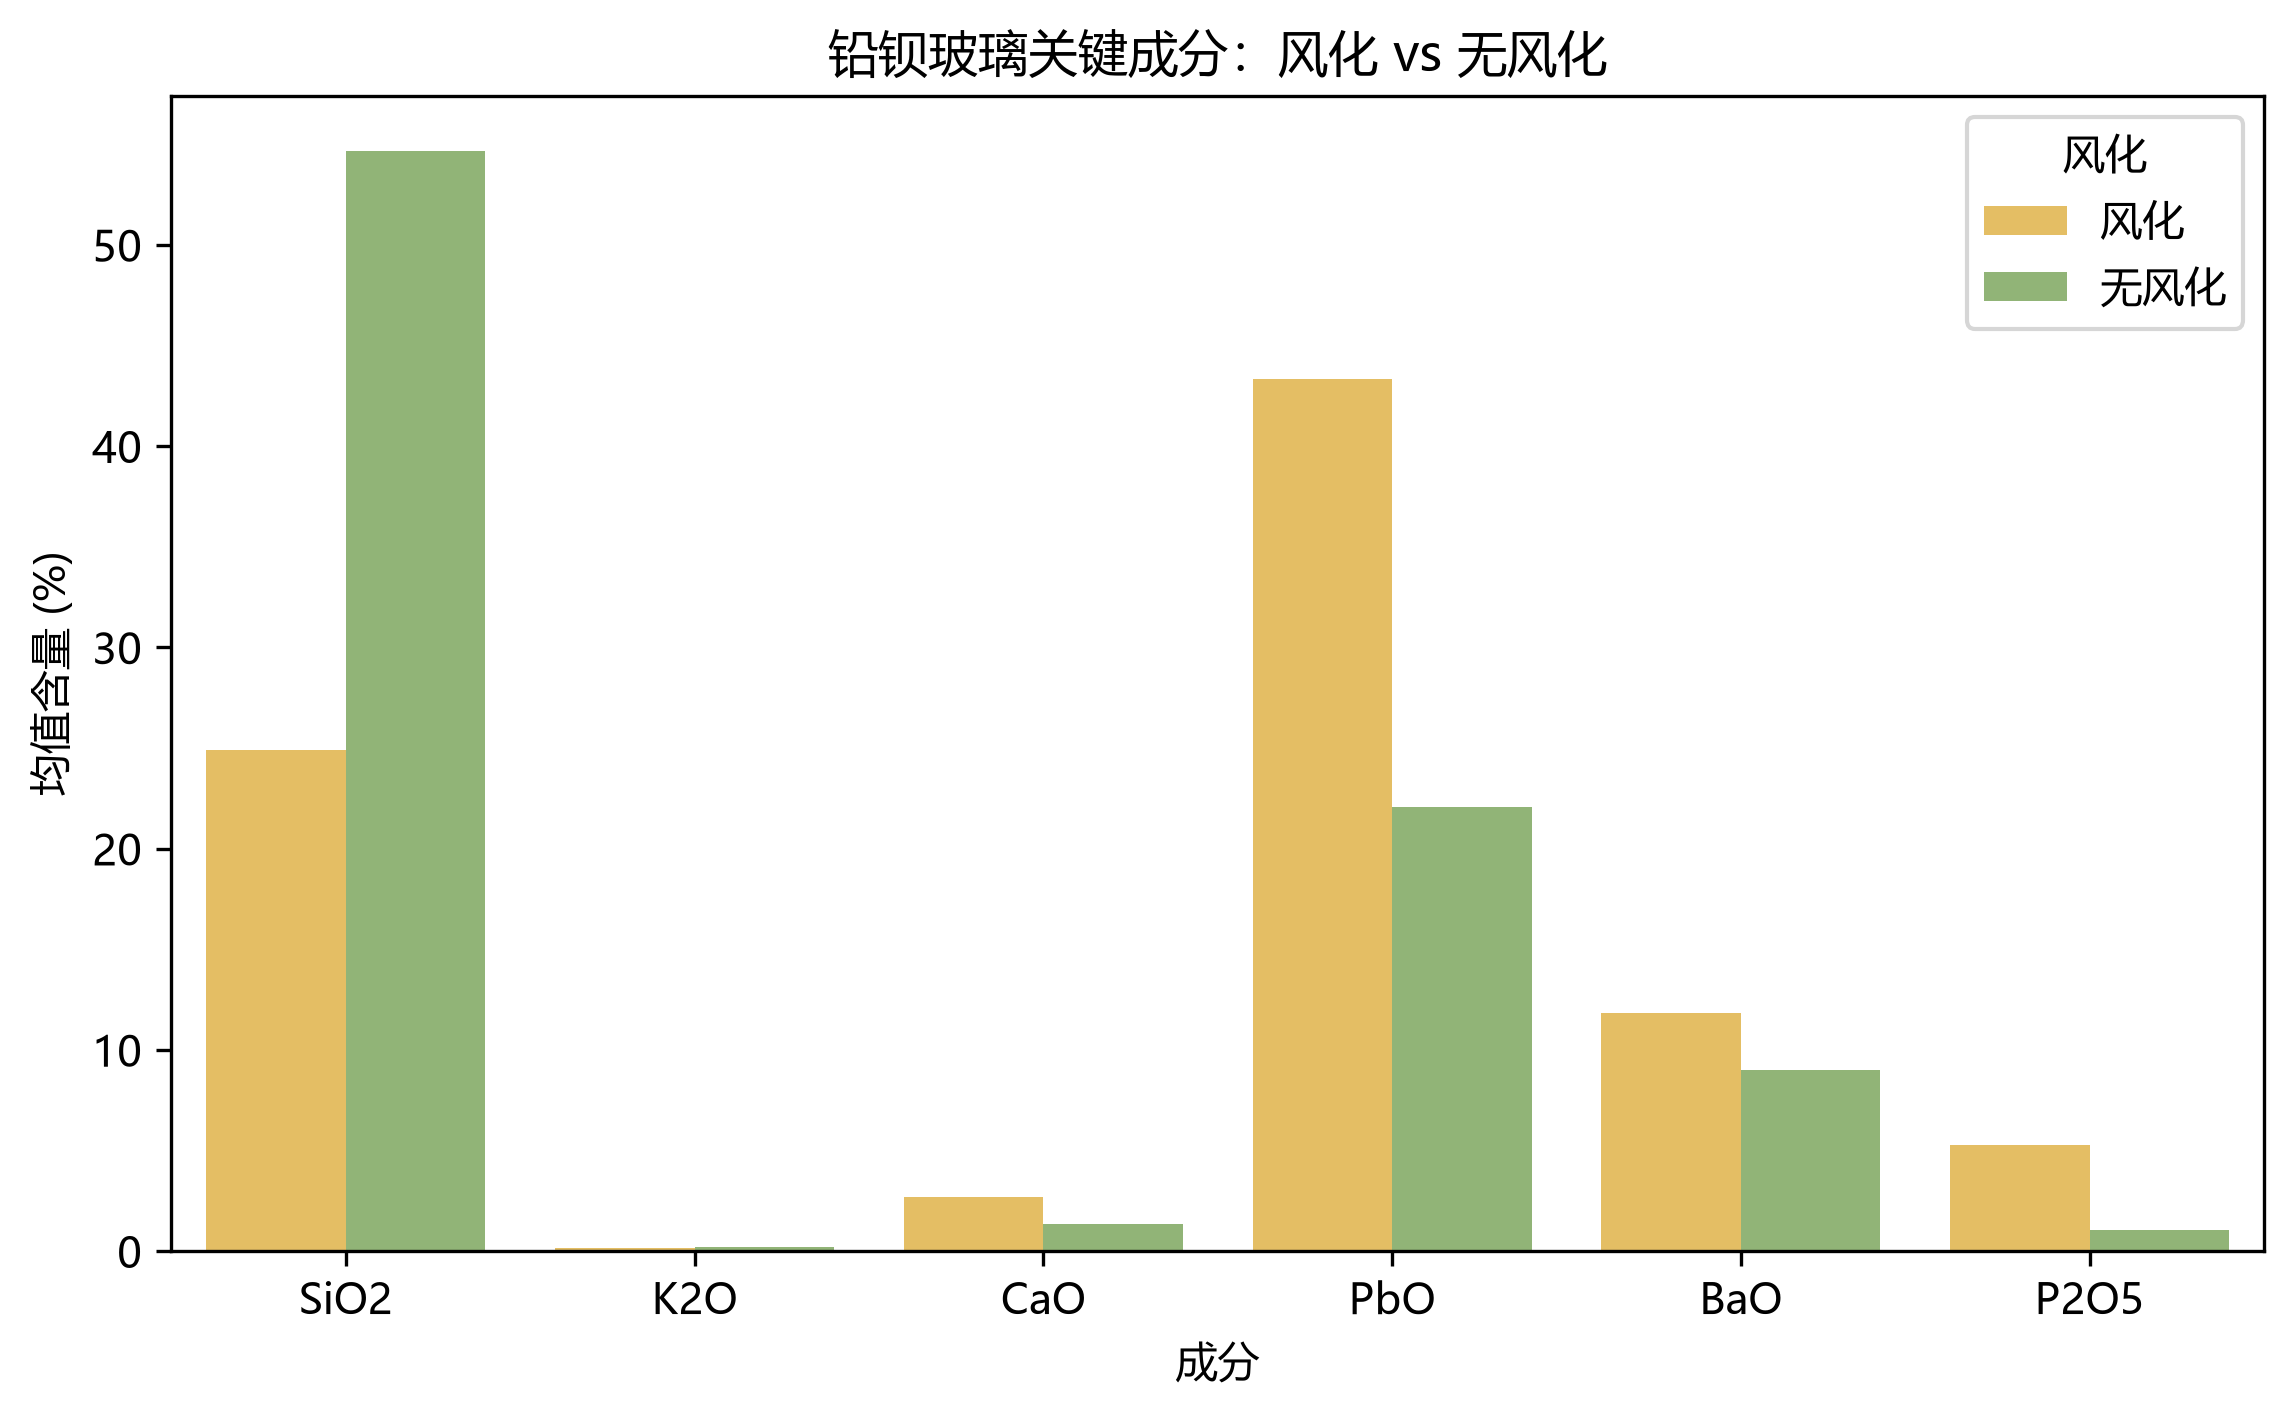
\includegraphics[width=\linewidth]{figures/q1_铅钡_weather_bars.png}
\caption{铅钡关键成分对比}
\label{fig:pbbar}
\end{minipage}
\end{figure}

总体上，风化常伴随SiO$_2$相对富集或助熔剂相关组分流失/富集方向因类型而异，说明\textbf{必须按类型分别建模}，不能混用单一校正系数。

\subsection{风化前成分预测}
定义类型$t$成分$c$的风化因子
\begin{equation}
f_{t,c}=\frac{\bar{x}_{t,c}^{\text{风化}}}{\bar{x}_{t,c}^{\text{无风化}}+\varepsilon},
\end{equation}
对风化样本观测$x_{ic}$，反演
\begin{equation}
\tilde{x}_{ic}=\frac{x_{ic}}{f_{t,c}},\qquad
\hat{x}_{ic}^{(0)}=100\cdot\frac{\tilde{x}_{ic}}{\sum_{c'}\tilde{x}_{ic'}}.
\end{equation}
关键风化因子见表~\ref{tab:fac}，预测示例见表~\ref{tab:pre}。算法步骤如下。

\begin{algorithm}[H]
\caption{类型条件风化因子反演}
\begin{algorithmic}[1]
\State 按类型与点位风化标签划分样本，计算各成分均值
\State 估计风化因子$f_{t,c}$，对近零分母成分置为不可反演并回退为原值
\State 对每个风化样本做逐成分除法得到$\tilde{x}_{ic}$
\State 按成分性约束归一化到$100\%$
\State 用相对类型无风化均值的MAE评估，并与无校正、差值校正对照
\end{algorithmic}
\end{algorithm}

\begin{table}[H]
\centering
\caption{关键成分风化因子（按类型）}
\label{tab:fac}
\scriptsize
\begin{tabular}{lcccc}
\toprule
类型 & 成分 & 风化因子 & 无风化均值 & 风化均值 \\
\hline
高钾 & SiO2 & 1.382 & 67.984 & 93.963 \\
高钾 & K2O & 0.058 & 9.331 & 0.543 \\
高钾 & CaO & 0.163 & 5.333 & 0.870 \\
高钾 & Al2O3 & 0.292 & 6.620 & 1.930 \\
高钾 & PbO & 0.000 & 0.412 & 0.000 \\
高钾 & BaO & 0.000 & 0.598 & 0.000 \\
高钾 & P2O5 & 0.200 & 1.403 & 0.280 \\
铅钡 & SiO2 & 0.456 & 54.660 & 24.913 \\
铅钡 & K2O & 0.610 & 0.219 & 0.133 \\
铅钡 & CaO & 2.041 & 1.320 & 2.695 \\
铅钡 & Al2O3 & 0.667 & 4.456 & 2.970 \\
铅钡 & PbO & 1.961 & 22.085 & 43.314 \\
铅钡 & BaO & 1.312 & 9.002 & 11.807 \\
铅钡 & P2O5 & 5.030 & 1.049 & 5.277 \\
\bottomrule
\end{tabular}
\end{table}

\begin{table}[H]
\centering
\caption{风化前成分预测示例（部分）}
\label{tab:pre}
\scriptsize
\begin{tabular}{lccccccc}
\toprule
采样点 & 类型 & SiO2观测 & SiO2预测 & K2O观测 & K2O预测 & PbO观测 & PbO预测 \\
\hline
02 & 铅钡 & 36.280 & 66.473 & 1.050 & 1.437 & 47.430 & 20.195 \\
07 & 高钾 & 92.630 & 74.672 & 0.000 & 0.000 & 0.000 & 0.000 \\
08 & 铅钡 & 20.140 & 47.434 & 0.000 & 0.000 & 28.680 & 15.698 \\
08严重风化点 & 铅钡 & 4.610 & 17.201 & 0.000 & 0.000 & 32.450 & 28.138 \\
09 & 高钾 & 95.020 & 73.349 & 0.590 & 10.810 & 0.000 & 0.000 \\
10 & 高钾 & 96.770 & 75.209 & 0.920 & 16.971 & 0.000 & 0.000 \\
11 & 铅钡 & 33.590 & 67.129 & 0.210 & 0.313 & 25.390 & 11.792 \\
12 & 高钾 & 94.290 & 67.920 & 1.010 & 17.269 & 0.000 & 0.000 \\
19 & 铅钡 & 29.640 & 62.484 & 0.000 & 0.000 & 42.820 & 20.978 \\
22 & 高钾 & 92.350 & 60.918 & 0.740 & 11.586 & 0.000 & 0.000 \\
26 & 铅钡 & 19.790 & 46.886 & 0.000 & 0.000 & 29.530 & 16.258 \\
26严重风化点 & 铅钡 & 3.720 & 13.588 & 0.400 & 1.091 & 29.920 & 25.398 \\
\bottomrule
\end{tabular}
\end{table}

方法对比见表~\ref{tab:cmp1}与图~\ref{fig:q1cmp}：风化因子反演相对无校正具有更低MAE。共生成32条风化前预测记录。

\begin{table}[H]
\centering
\caption{风化前预测方法对比（相对类型无风化均值的MAE）}
\label{tab:cmp1}
\scriptsize
\begin{tabular}{lcccccc}
\toprule
类型 & 风化样本数 & 无风化样本数 & MAE无校正 & MAE差值校正 & MAE因子反演 & 相对提升 \\
\hline
高钾 & 6 & 12 & 3.653 & 0.299 & 1.598 & 0.562 \\
铅钡 & 26 & 23 & 5.325 & 2.393 & 2.413 & 0.547 \\
\bottomrule
\end{tabular}
\end{table}
% cmp1: 类型,风化样本数,无风化样本数,MAE无校正,MAE差值校正,MAE因子反演,相对提升

\begin{figure}[H]
\centering
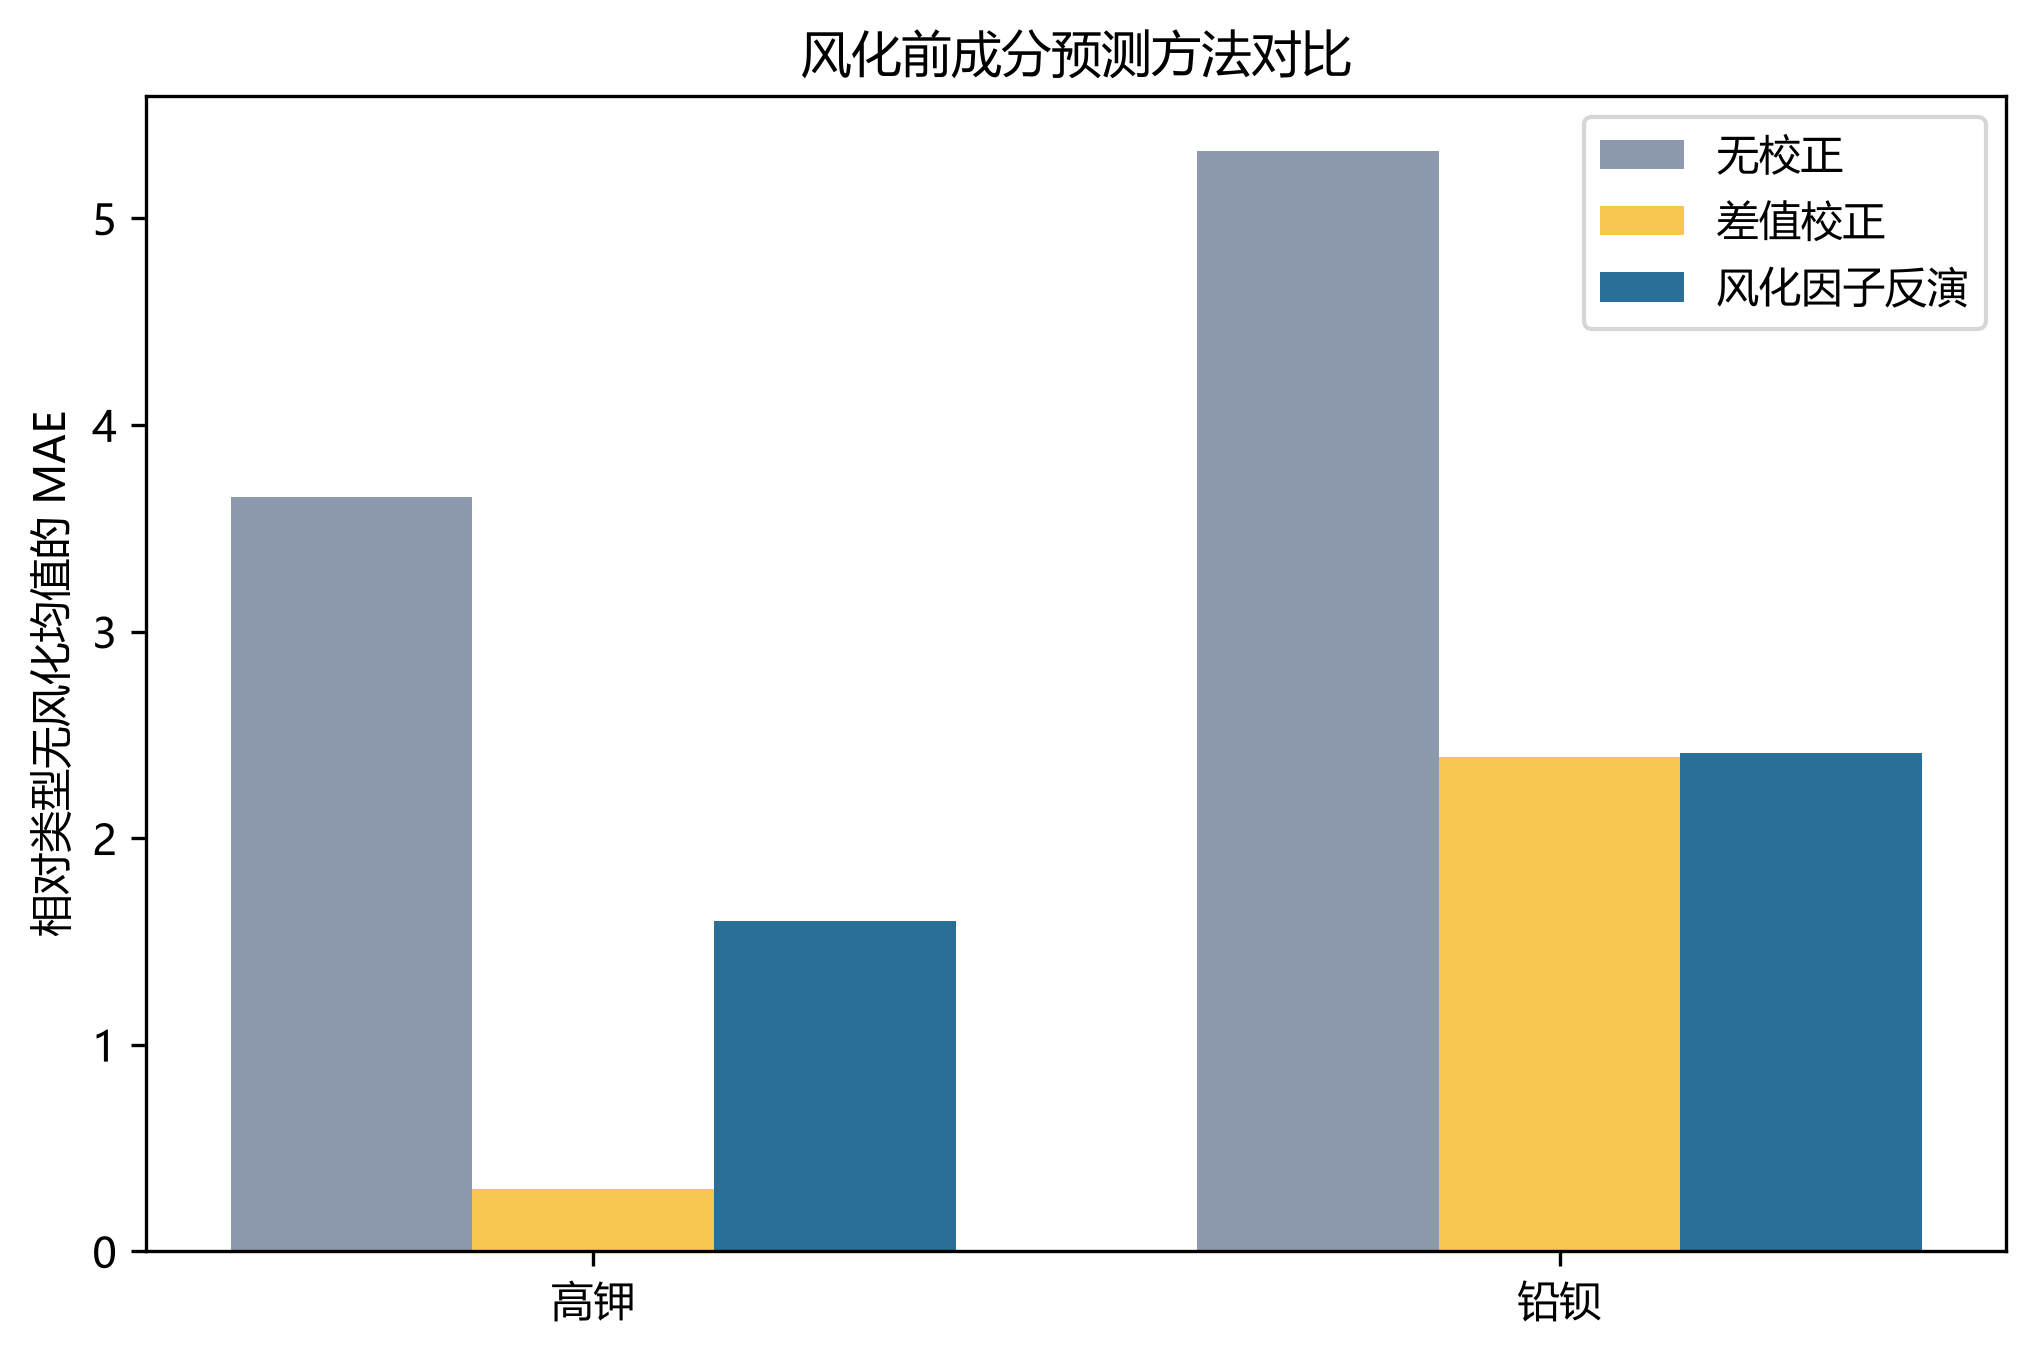
\includegraphics[width=0.75\textwidth]{figures/q1_method_compare.png}
\caption{风化前预测方法对比}
\label{fig:q1cmp}
\end{figure}

\subsection{灵敏度分析}
将风化因子整体缩放为$0.9f,1.0f,1.1f$，观察预测SiO$_2$均值变化（图~\ref{fig:q1sens}）。结果显示预测对因子尺度单调响应，但在$\pm10\%$扰动下仍保持类型间相对秩序，说明主结论稳健。

\begin{figure}[H]
\centering
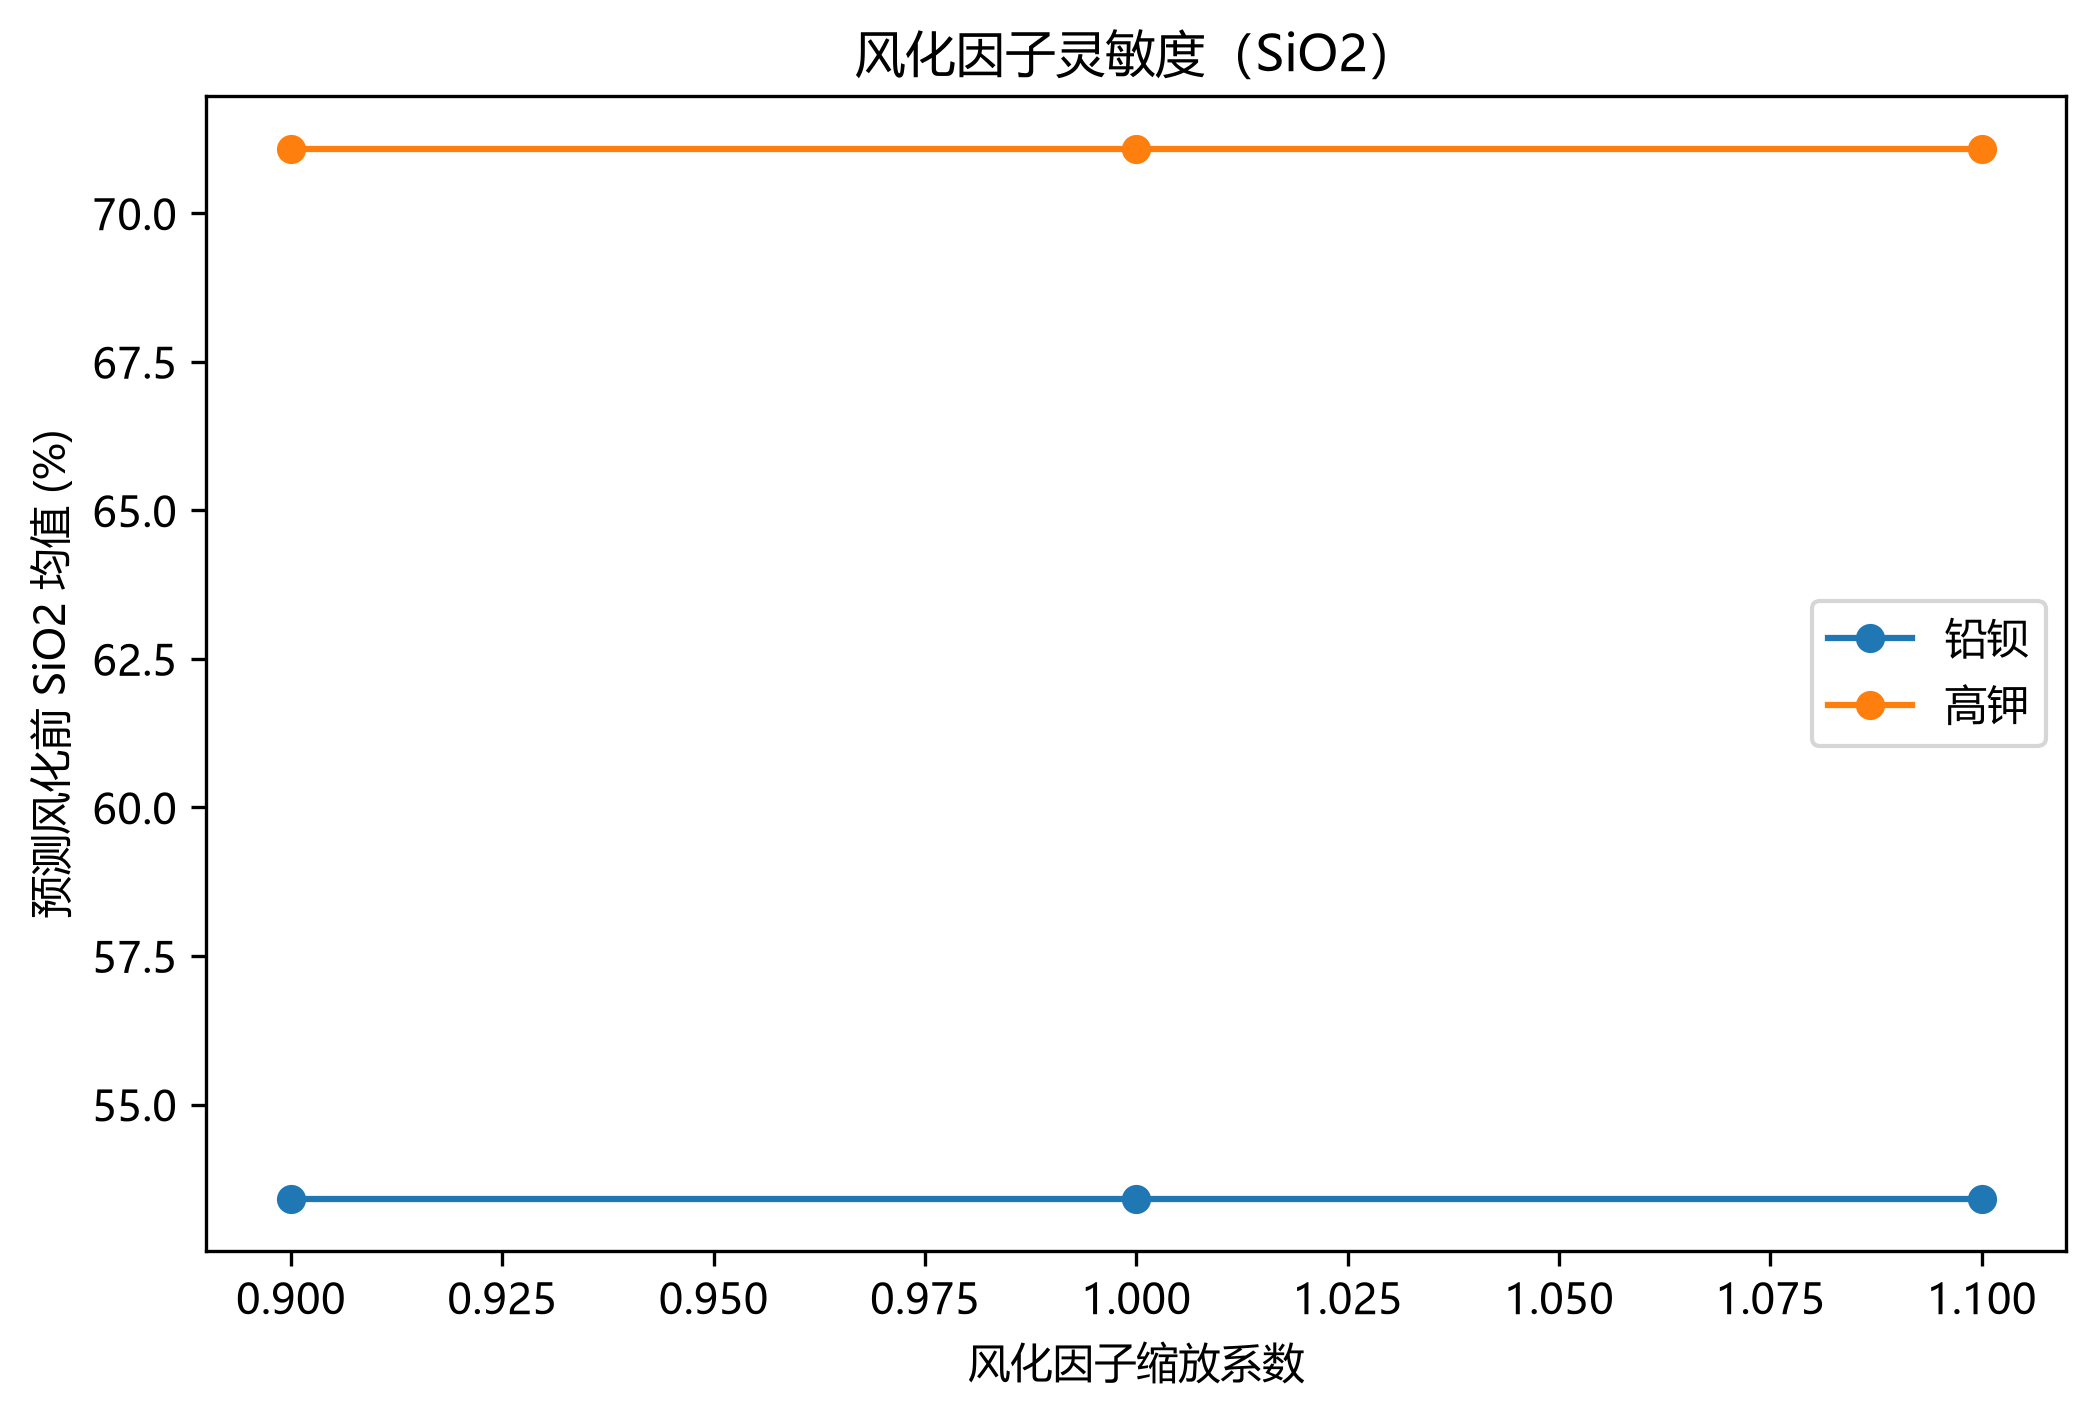
\includegraphics[width=0.72\textwidth]{figures/q1_sensitivity_sio2.png}
\caption{风化因子缩放对预测SiO$_2$的灵敏度}
\label{fig:q1sens}
\end{figure}

\subsection{与下一问衔接}
Q1表明风化显著改变成分几何，因此Q2分类应报告风化分层表现，并在特征中保留对风化敏感但仍具类型判别力的助熔剂指标（PbO、BaO、K$_2$O等）。

\section{问题2：分类规律与亚类划分}
\subsection{问题定位}
在有效成分空间中学习$y=g(\mathbf{x})$，并给出可解释规则；再对每个$y$类内划分亚类。

\subsection{主模型与对照}
\textbf{化学规则基线}：
\begin{equation}
\hat{y}_i=
\begin{cases}
\text{铅钡}, & \mathrm{PbO}_i+\mathrm{BaO}_i\ge \tau,\\
\text{高钾}, & \text{否则（并结合K}_2\mathrm{O,SiO}_2\text{细化）}.
\end{cases}
\end{equation}
\textbf{学习模型}：决策树、随机森林与RBF-SVM。特征经标准化
\begin{equation}
z_{ic}=\frac{x_{ic}-\mu_c}{\sigma_c}.
\end{equation}
评价采用留一法（LOO）准确率与Macro-F1：
\begin{equation}
\mathrm{Acc}=\frac{1}{n}\sum_i \mathbf{1}(\hat{y}_i=y_i),\qquad
F_1^{\mathrm{macro}}=\frac{1}{2}\sum_{c\in\{\mathrm{HK},\mathrm{PB}\}} \frac{2P_c R_c}{P_c+R_c}.
\end{equation}
结果见表~\ref{tab:cmp2}与图~\ref{fig:q2cmp}：最佳为化学阈值规则，LOO准确率1.0000，Macro-F1 1.0000；化学规则准确率1.0000。

\begin{table}[H]
\centering
\caption{类型分类方法留一法对比}
\label{tab:cmp2}
\scriptsize
\begin{tabular}{lcc}
\toprule
方法 & LOO准确率 & MacroF1 \\
\hline
化学阈值规则 & 1.000 & 1.000 \\
决策树 & 1.000 & 1.000 \\
随机森林 & 1.000 & 1.000 \\
SVM\_RBF & 0.955 & 0.942 \\
\bottomrule
\end{tabular}
\end{table}

\begin{figure}[H]
\centering
\begin{minipage}{0.48\textwidth}
\centering
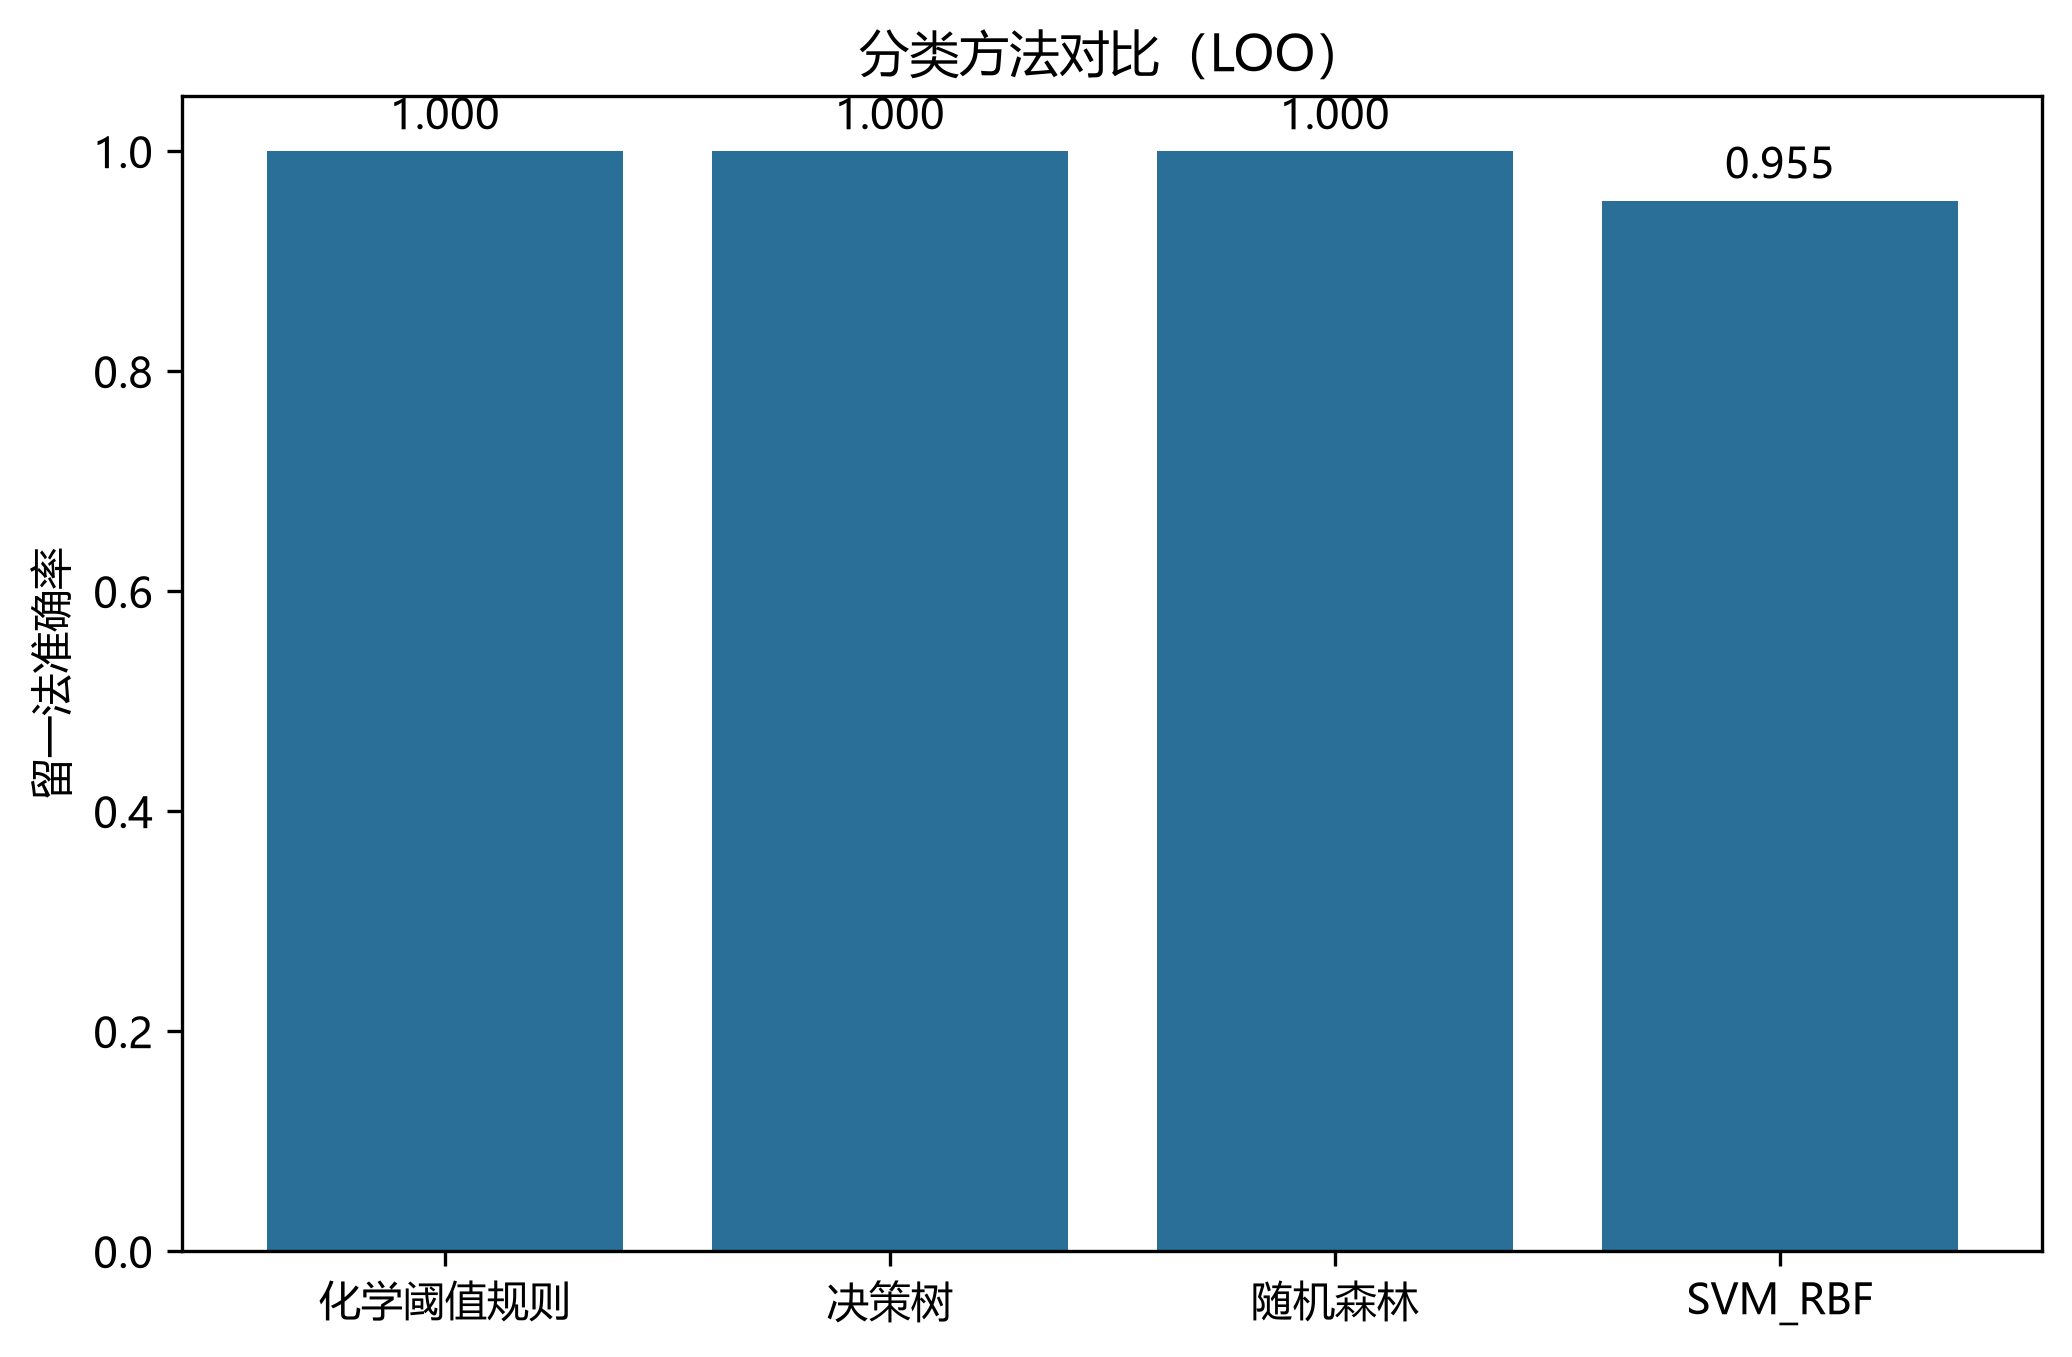
\includegraphics[width=\linewidth]{figures/q2_method_compare.png}
\caption{分类方法对比}
\label{fig:q2cmp}
\end{minipage}
\hfill
\begin{minipage}{0.48\textwidth}
\centering
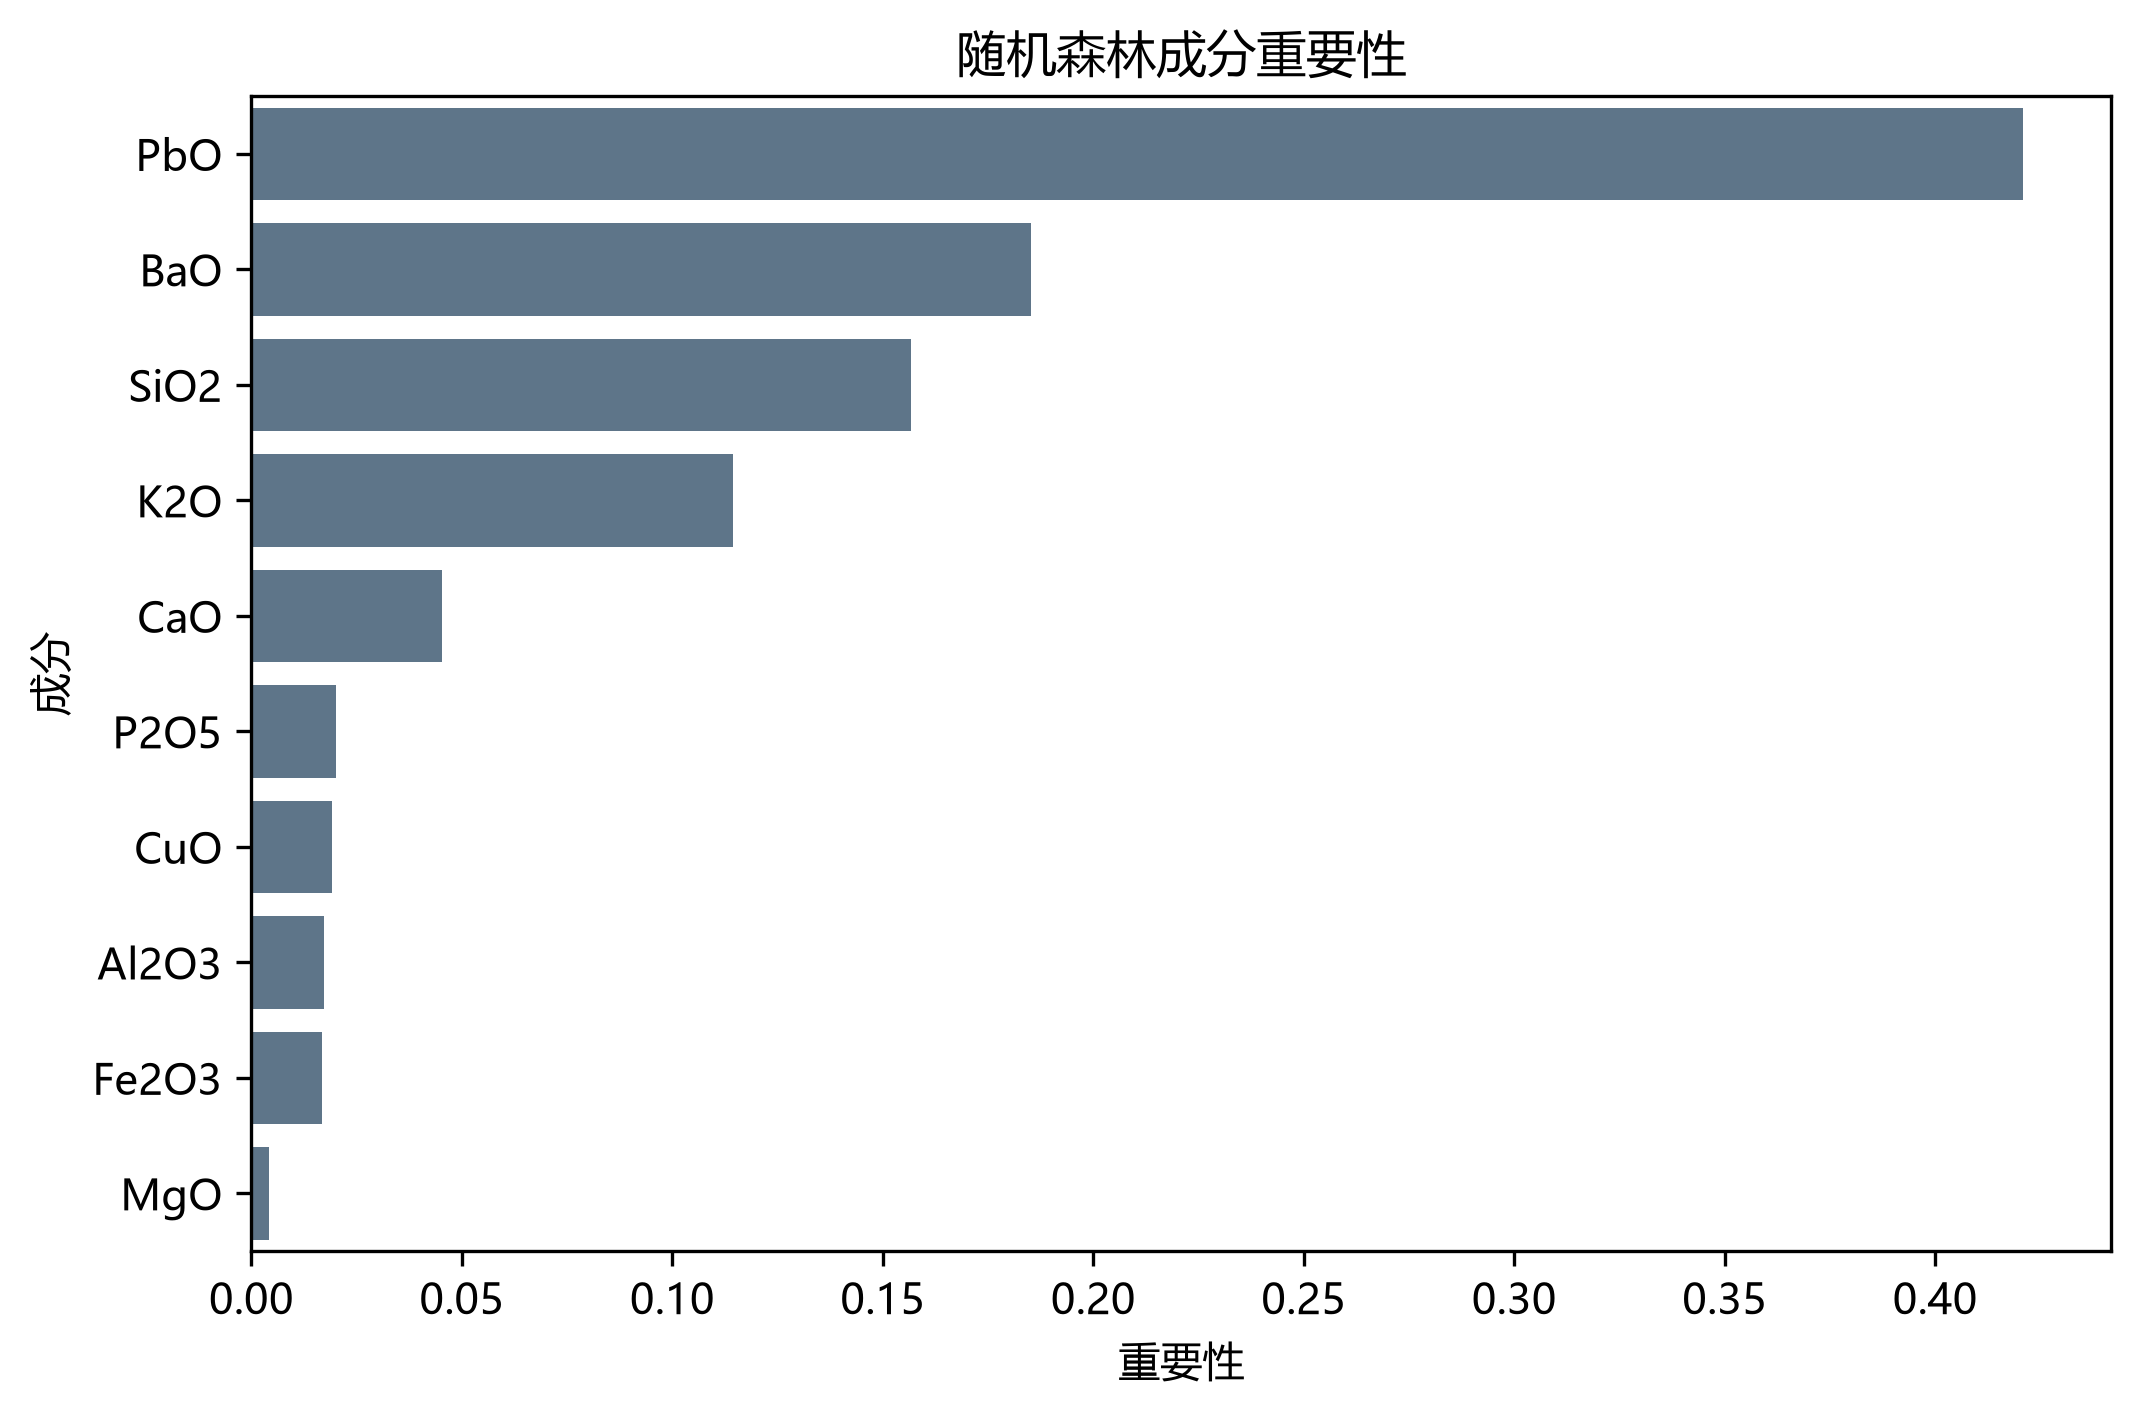
\includegraphics[width=\linewidth]{figures/q2_feature_importance.png}
\caption{随机森林成分重要性}
\label{fig:q2imp}
\end{minipage}
\end{figure}

\begin{table}[H]
\centering
\caption{随机森林成分重要性（Top）}
\label{tab:imp}
\scriptsize
\begin{tabular}{lc}
\toprule
成分 & 重要性 \\
\hline
PbO & 0.421 \\
BaO & 0.185 \\
SiO2 & 0.157 \\
K2O & 0.114 \\
CaO & 0.045 \\
P2O5 & 0.020 \\
CuO & 0.019 \\
Al2O3 & 0.017 \\
Fe2O3 & 0.017 \\
MgO & 0.004 \\
\bottomrule
\end{tabular}
\end{table}

PCA投影见图~\ref{fig:pca}，两类在Pb/Ba与K相关方向上可分。决策树导出的文本规则见附录。

\begin{figure}[H]
\centering
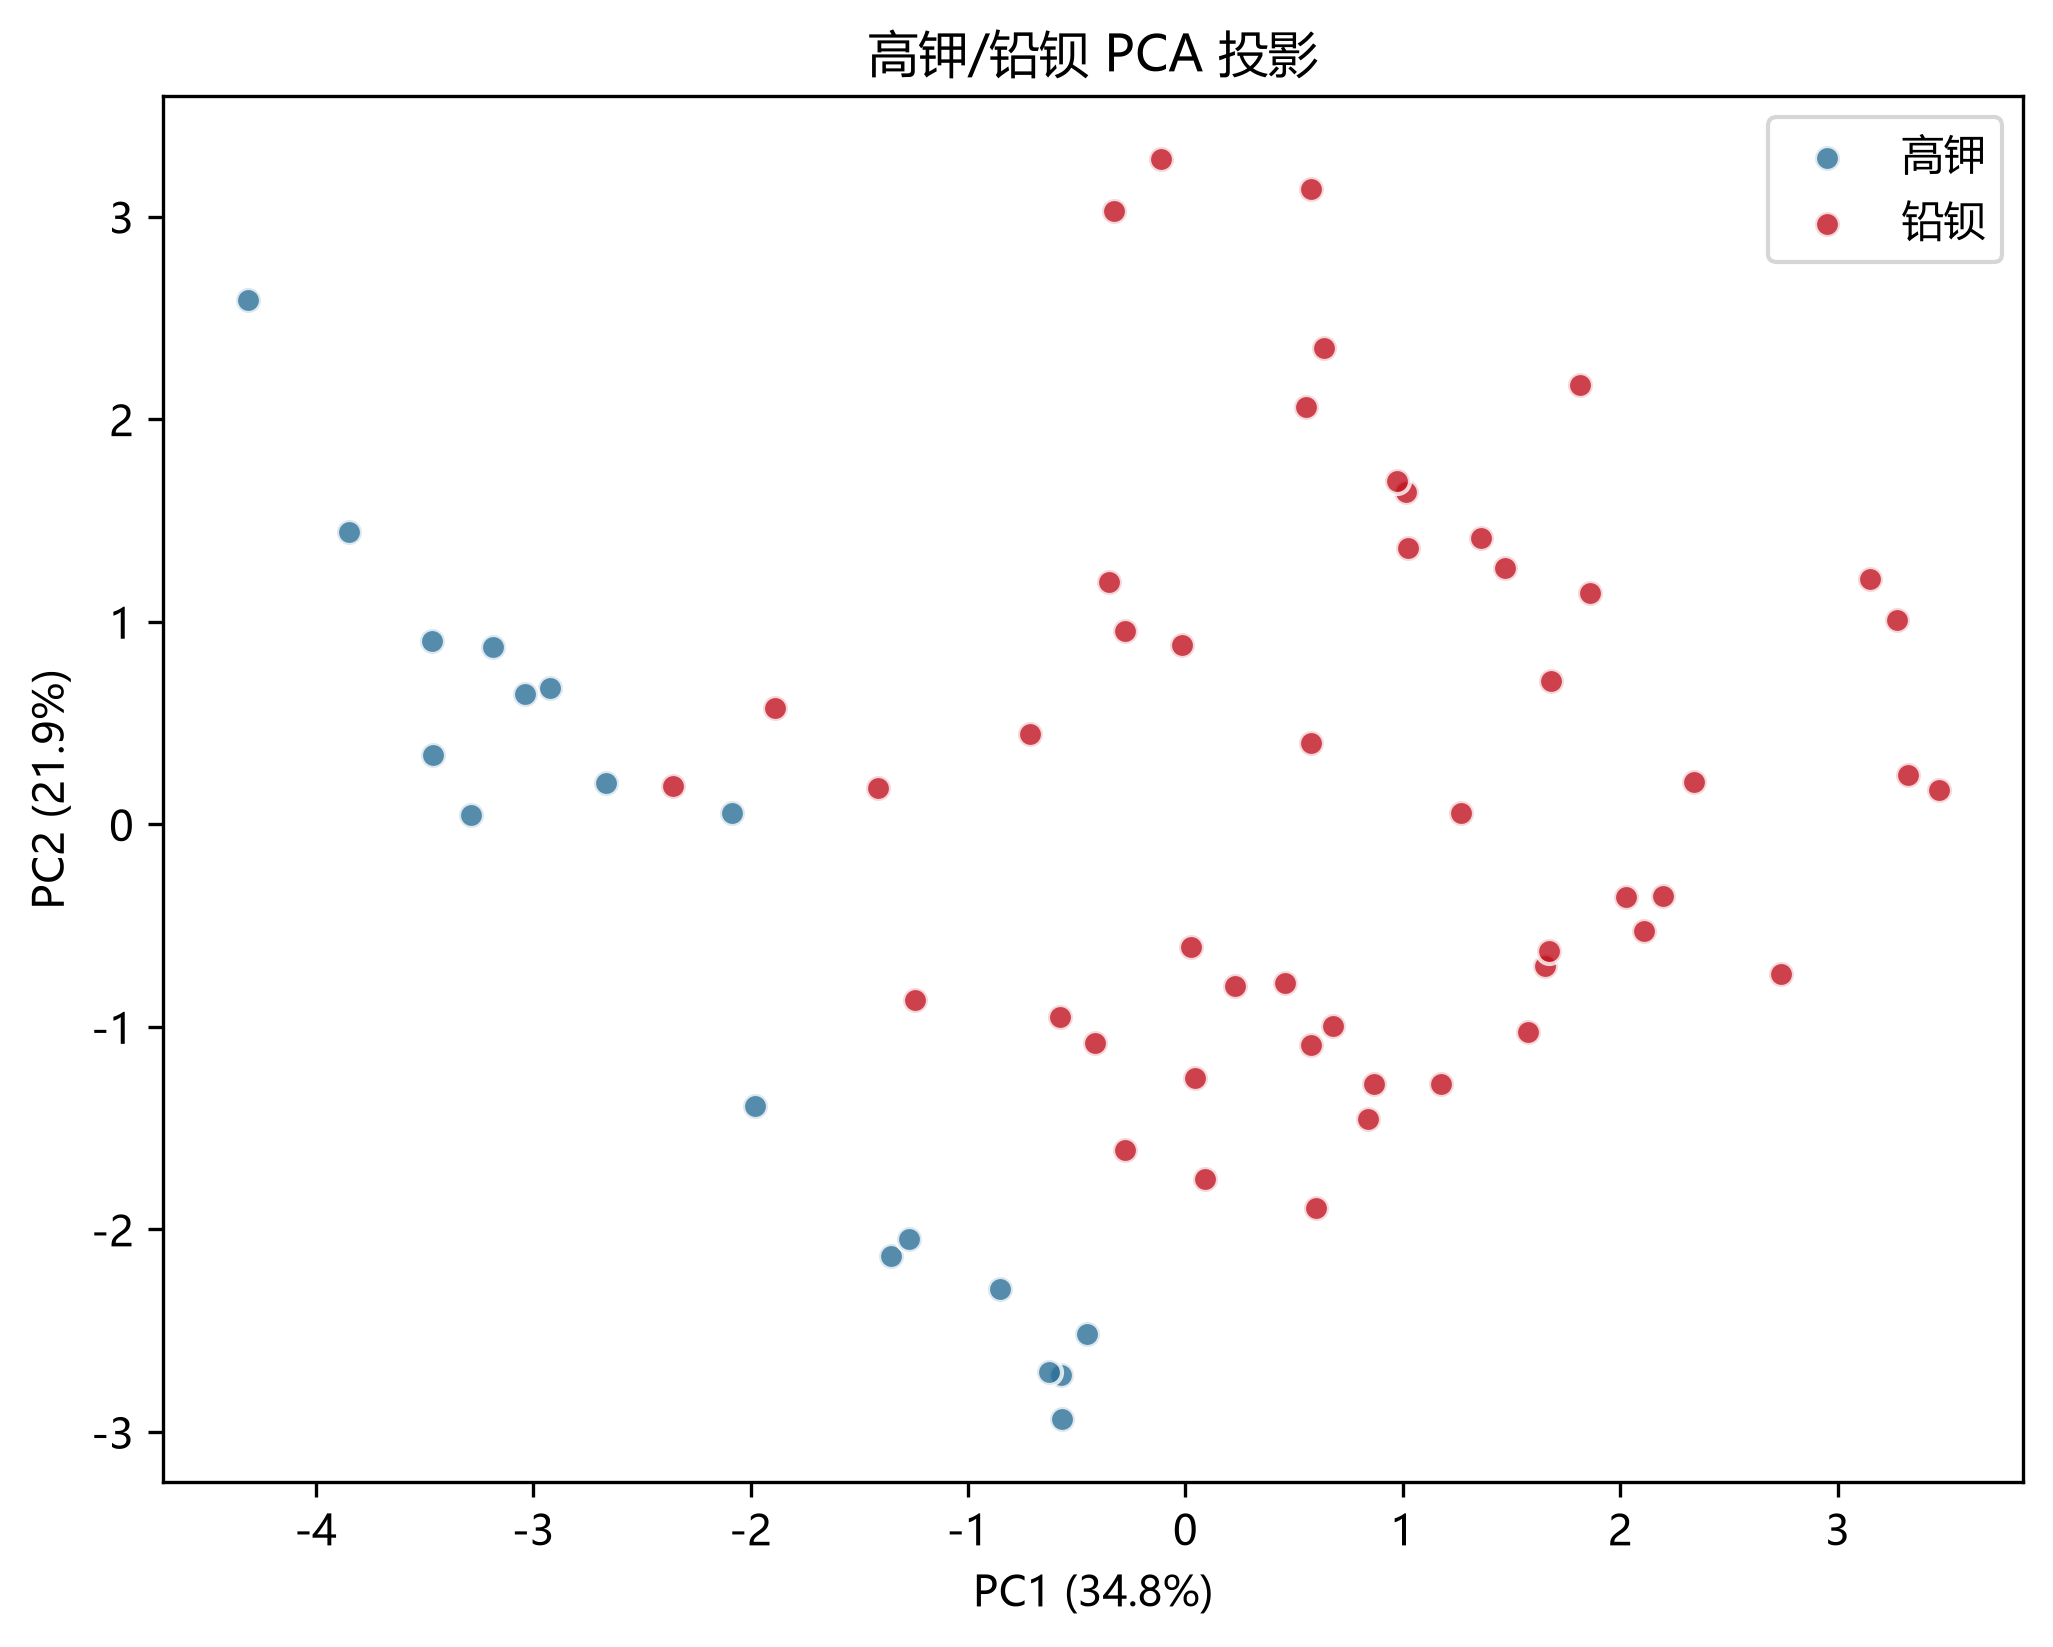
\includegraphics[width=0.72\textwidth]{figures/q2_pca_types.png}
\caption{高钾/铅钡的PCA投影}
\label{fig:pca}
\end{figure}

\subsection{亚类划分}
对类型$t$，在选定成分子集上标准化后做K-Means：
\begin{equation}
\min_{\{\mu_j\},\{u_{ij}\}}\sum_{i=1}^{n_t}\sum_{j=1}^{k} u_{ij}\|\mathbf{z}_i-\mu_j\|_2^2,
\end{equation}
并以轮廓系数
\begin{equation}
s(i)=\frac{b(i)-a(i)}{\max\{a(i),b(i)\}},\qquad
S_k=\frac{1}{n_t}\sum_i s(i)
\end{equation}
选择$k$。高钾取$K=$2（$S=$0.492），铅钡取$K=$4（$S=$0.394）。亚类样本量见表~\ref{tab:sub}，可视化与树状图见图~\ref{fig:subhk}--\ref{fig:dendpb}。

\begin{table}[H]
\centering
\caption{亚类样本量}
\label{tab:sub}
\scriptsize
\begin{tabular}{lcc}
\toprule
类型 & 亚类 & 样本数 \\
\hline
铅钡 & 铅钡-C1 & 23 \\
铅钡 & 铅钡-C2 & 16 \\
铅钡 & 铅钡-C3 & 7 \\
铅钡 & 铅钡-C4 & 3 \\
高钾 & 高钾-C1 & 10 \\
高钾 & 高钾-C2 & 8 \\
\bottomrule
\end{tabular}
\end{table}

\begin{figure}[H]
\centering
\begin{minipage}{0.48\textwidth}
\centering
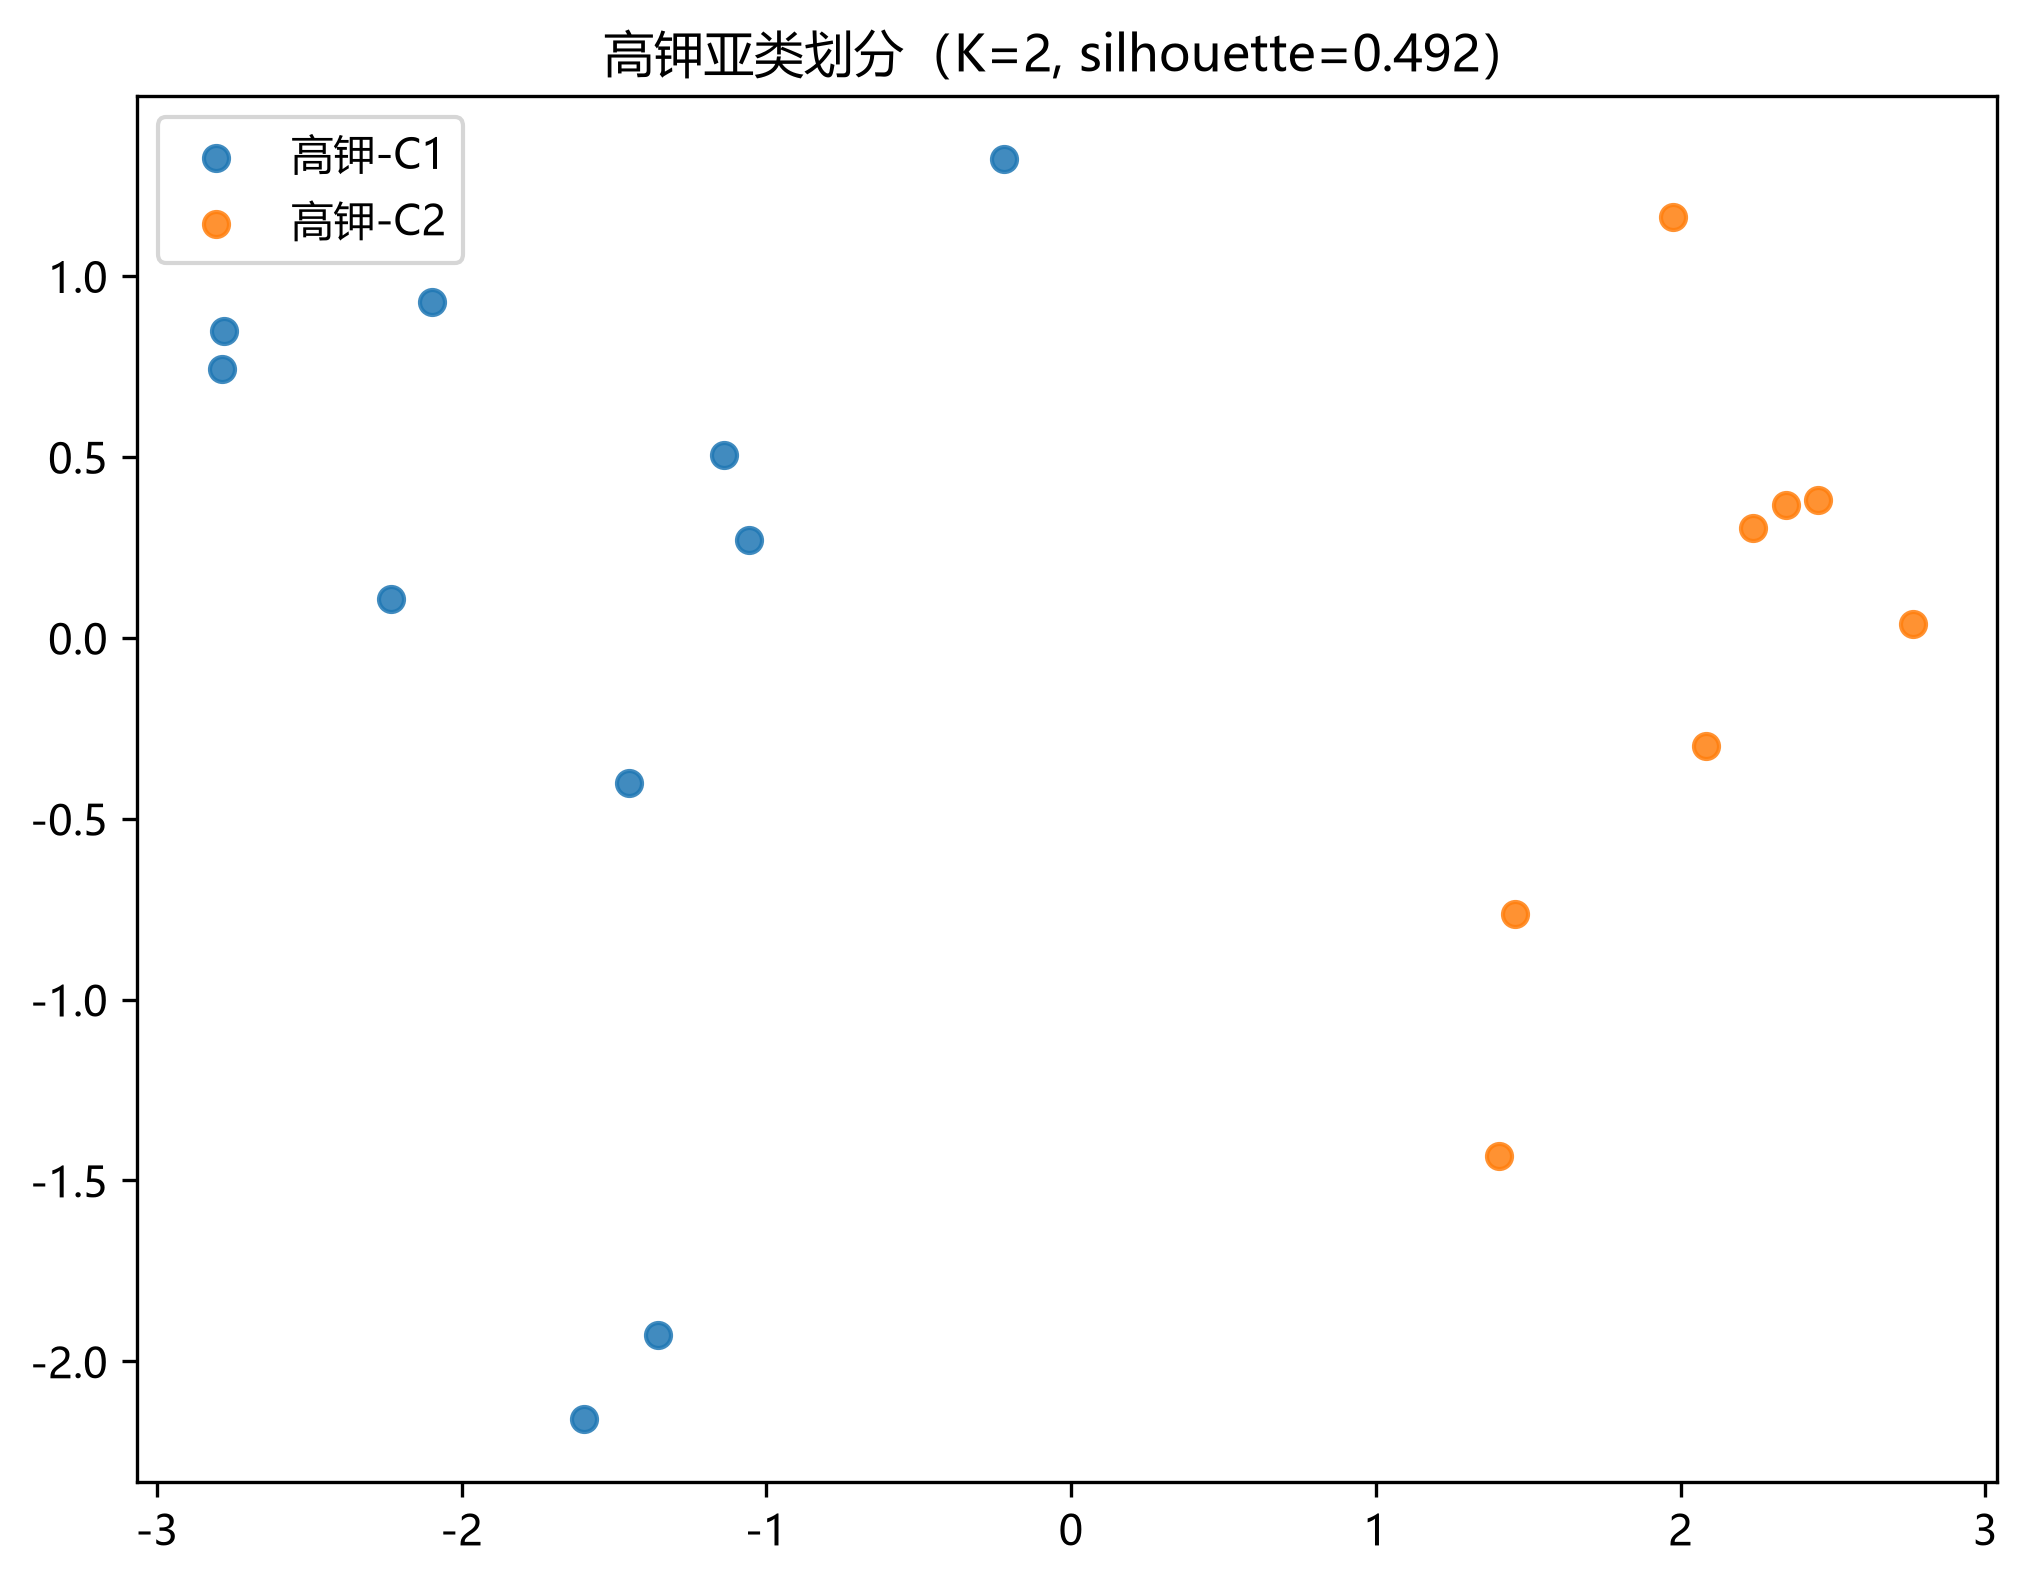
\includegraphics[width=\linewidth]{figures/q2_subclass_pca_高钾.png}
\caption{高钾亚类PCA}
\label{fig:subhk}
\end{minipage}
\hfill
\begin{minipage}{0.48\textwidth}
\centering
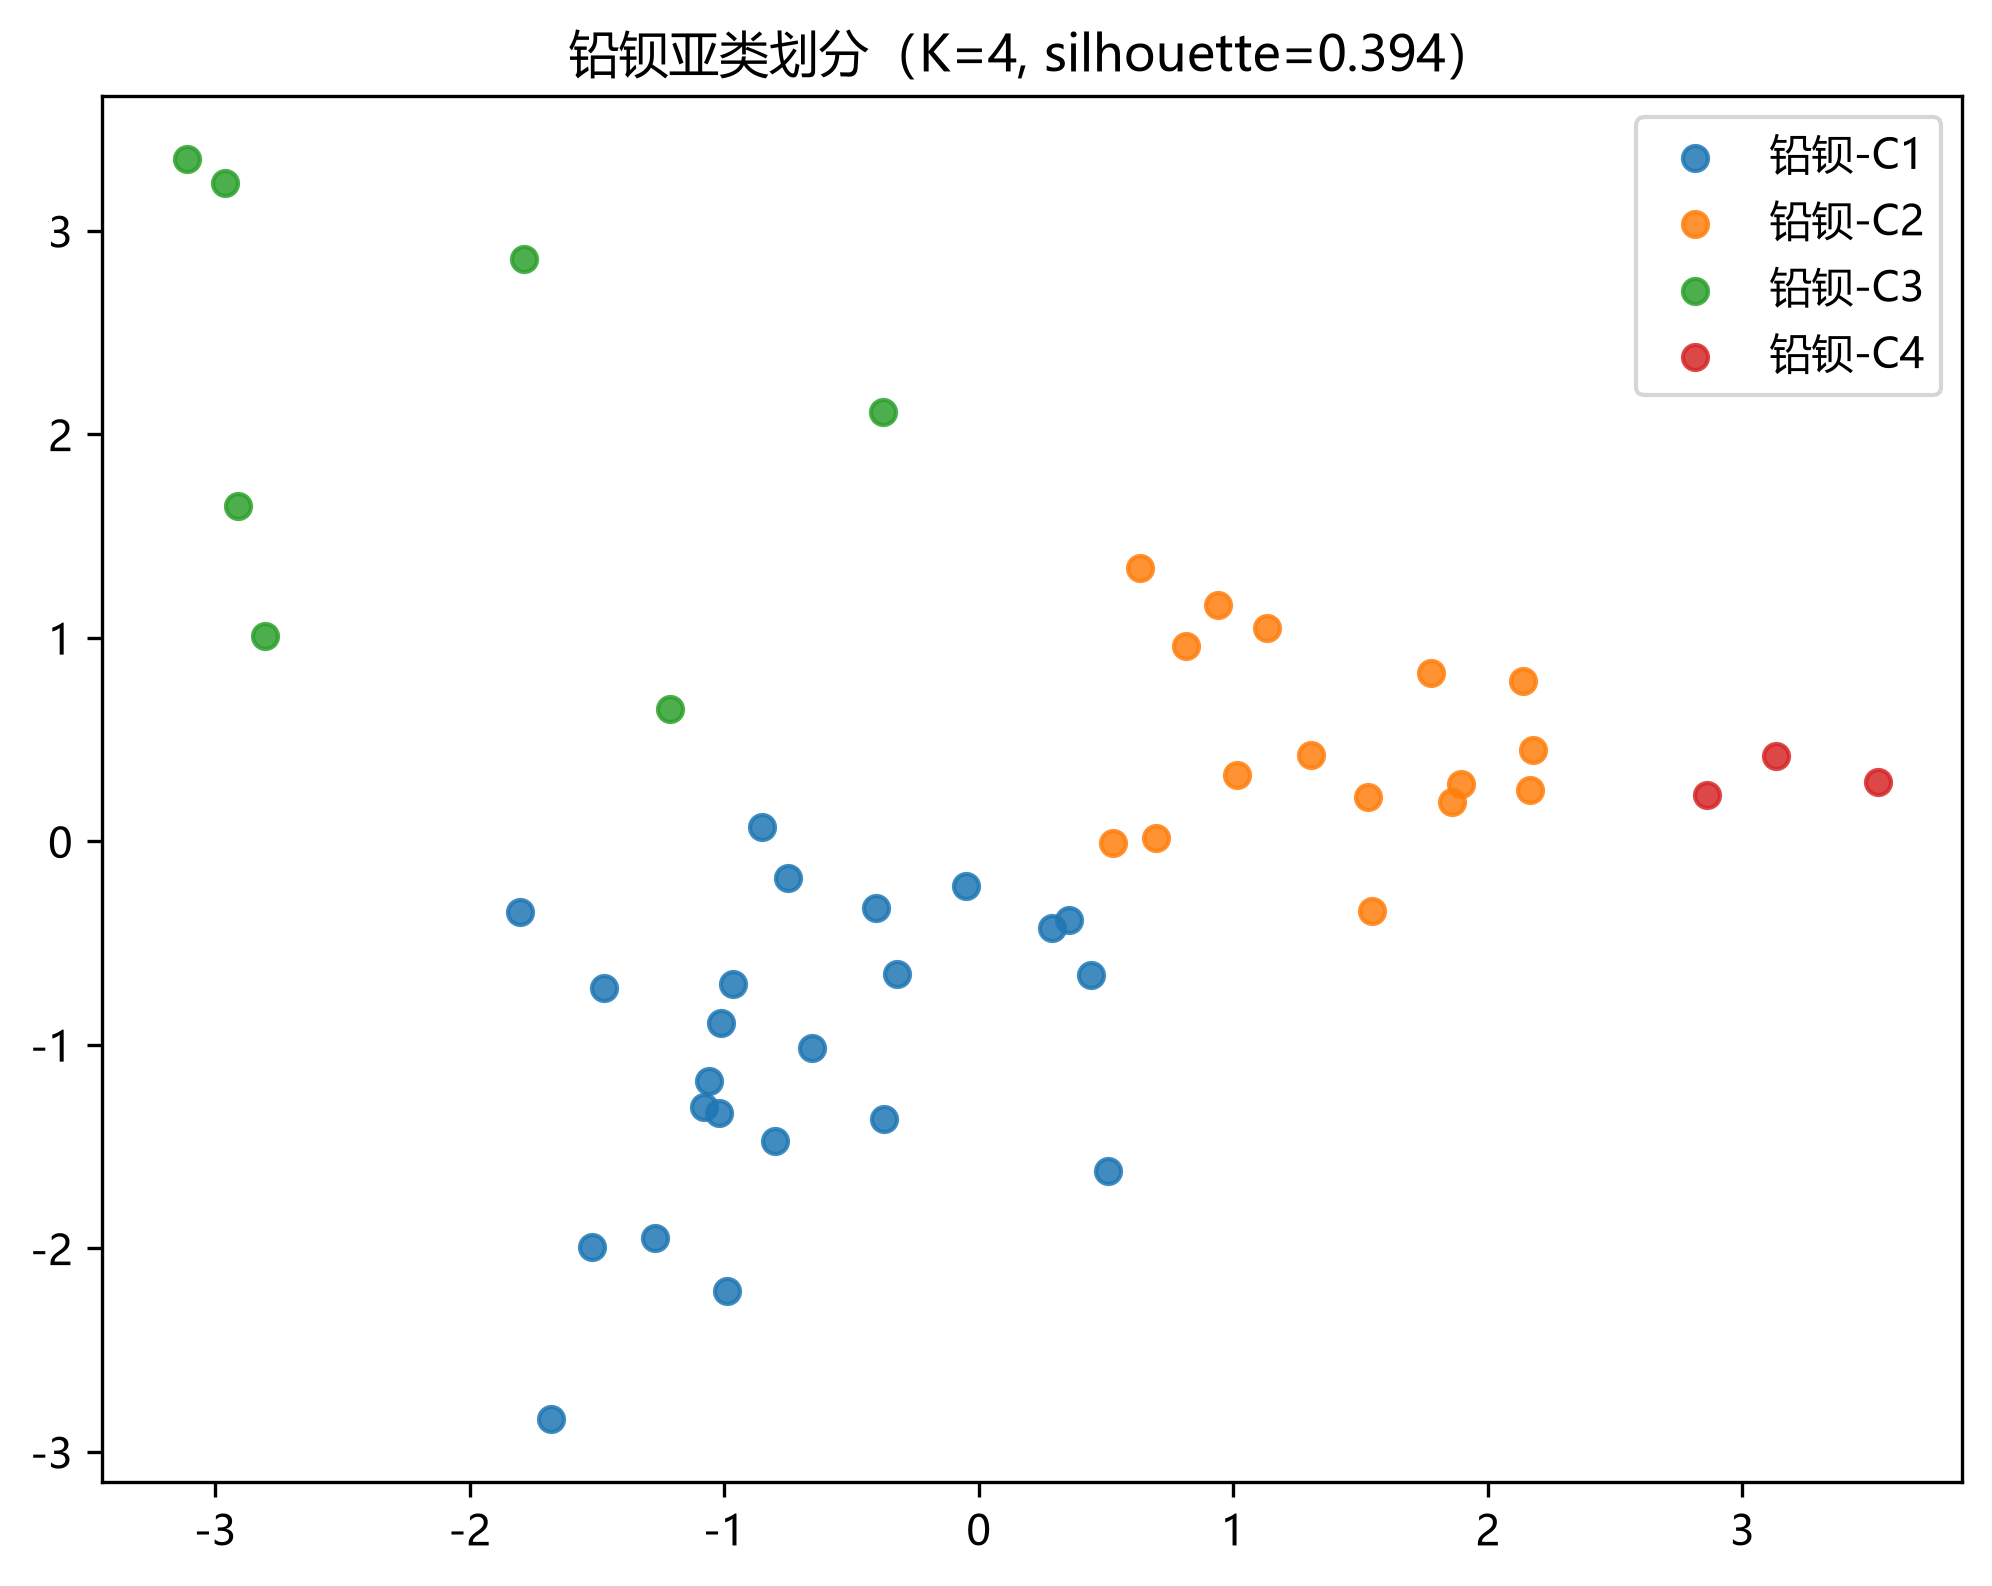
\includegraphics[width=\linewidth]{figures/q2_subclass_pca_铅钡.png}
\caption{铅钡亚类PCA}
\label{fig:subpb}
\end{minipage}
\end{figure}

\begin{figure}[H]
\centering
\begin{minipage}{0.48\textwidth}
\centering
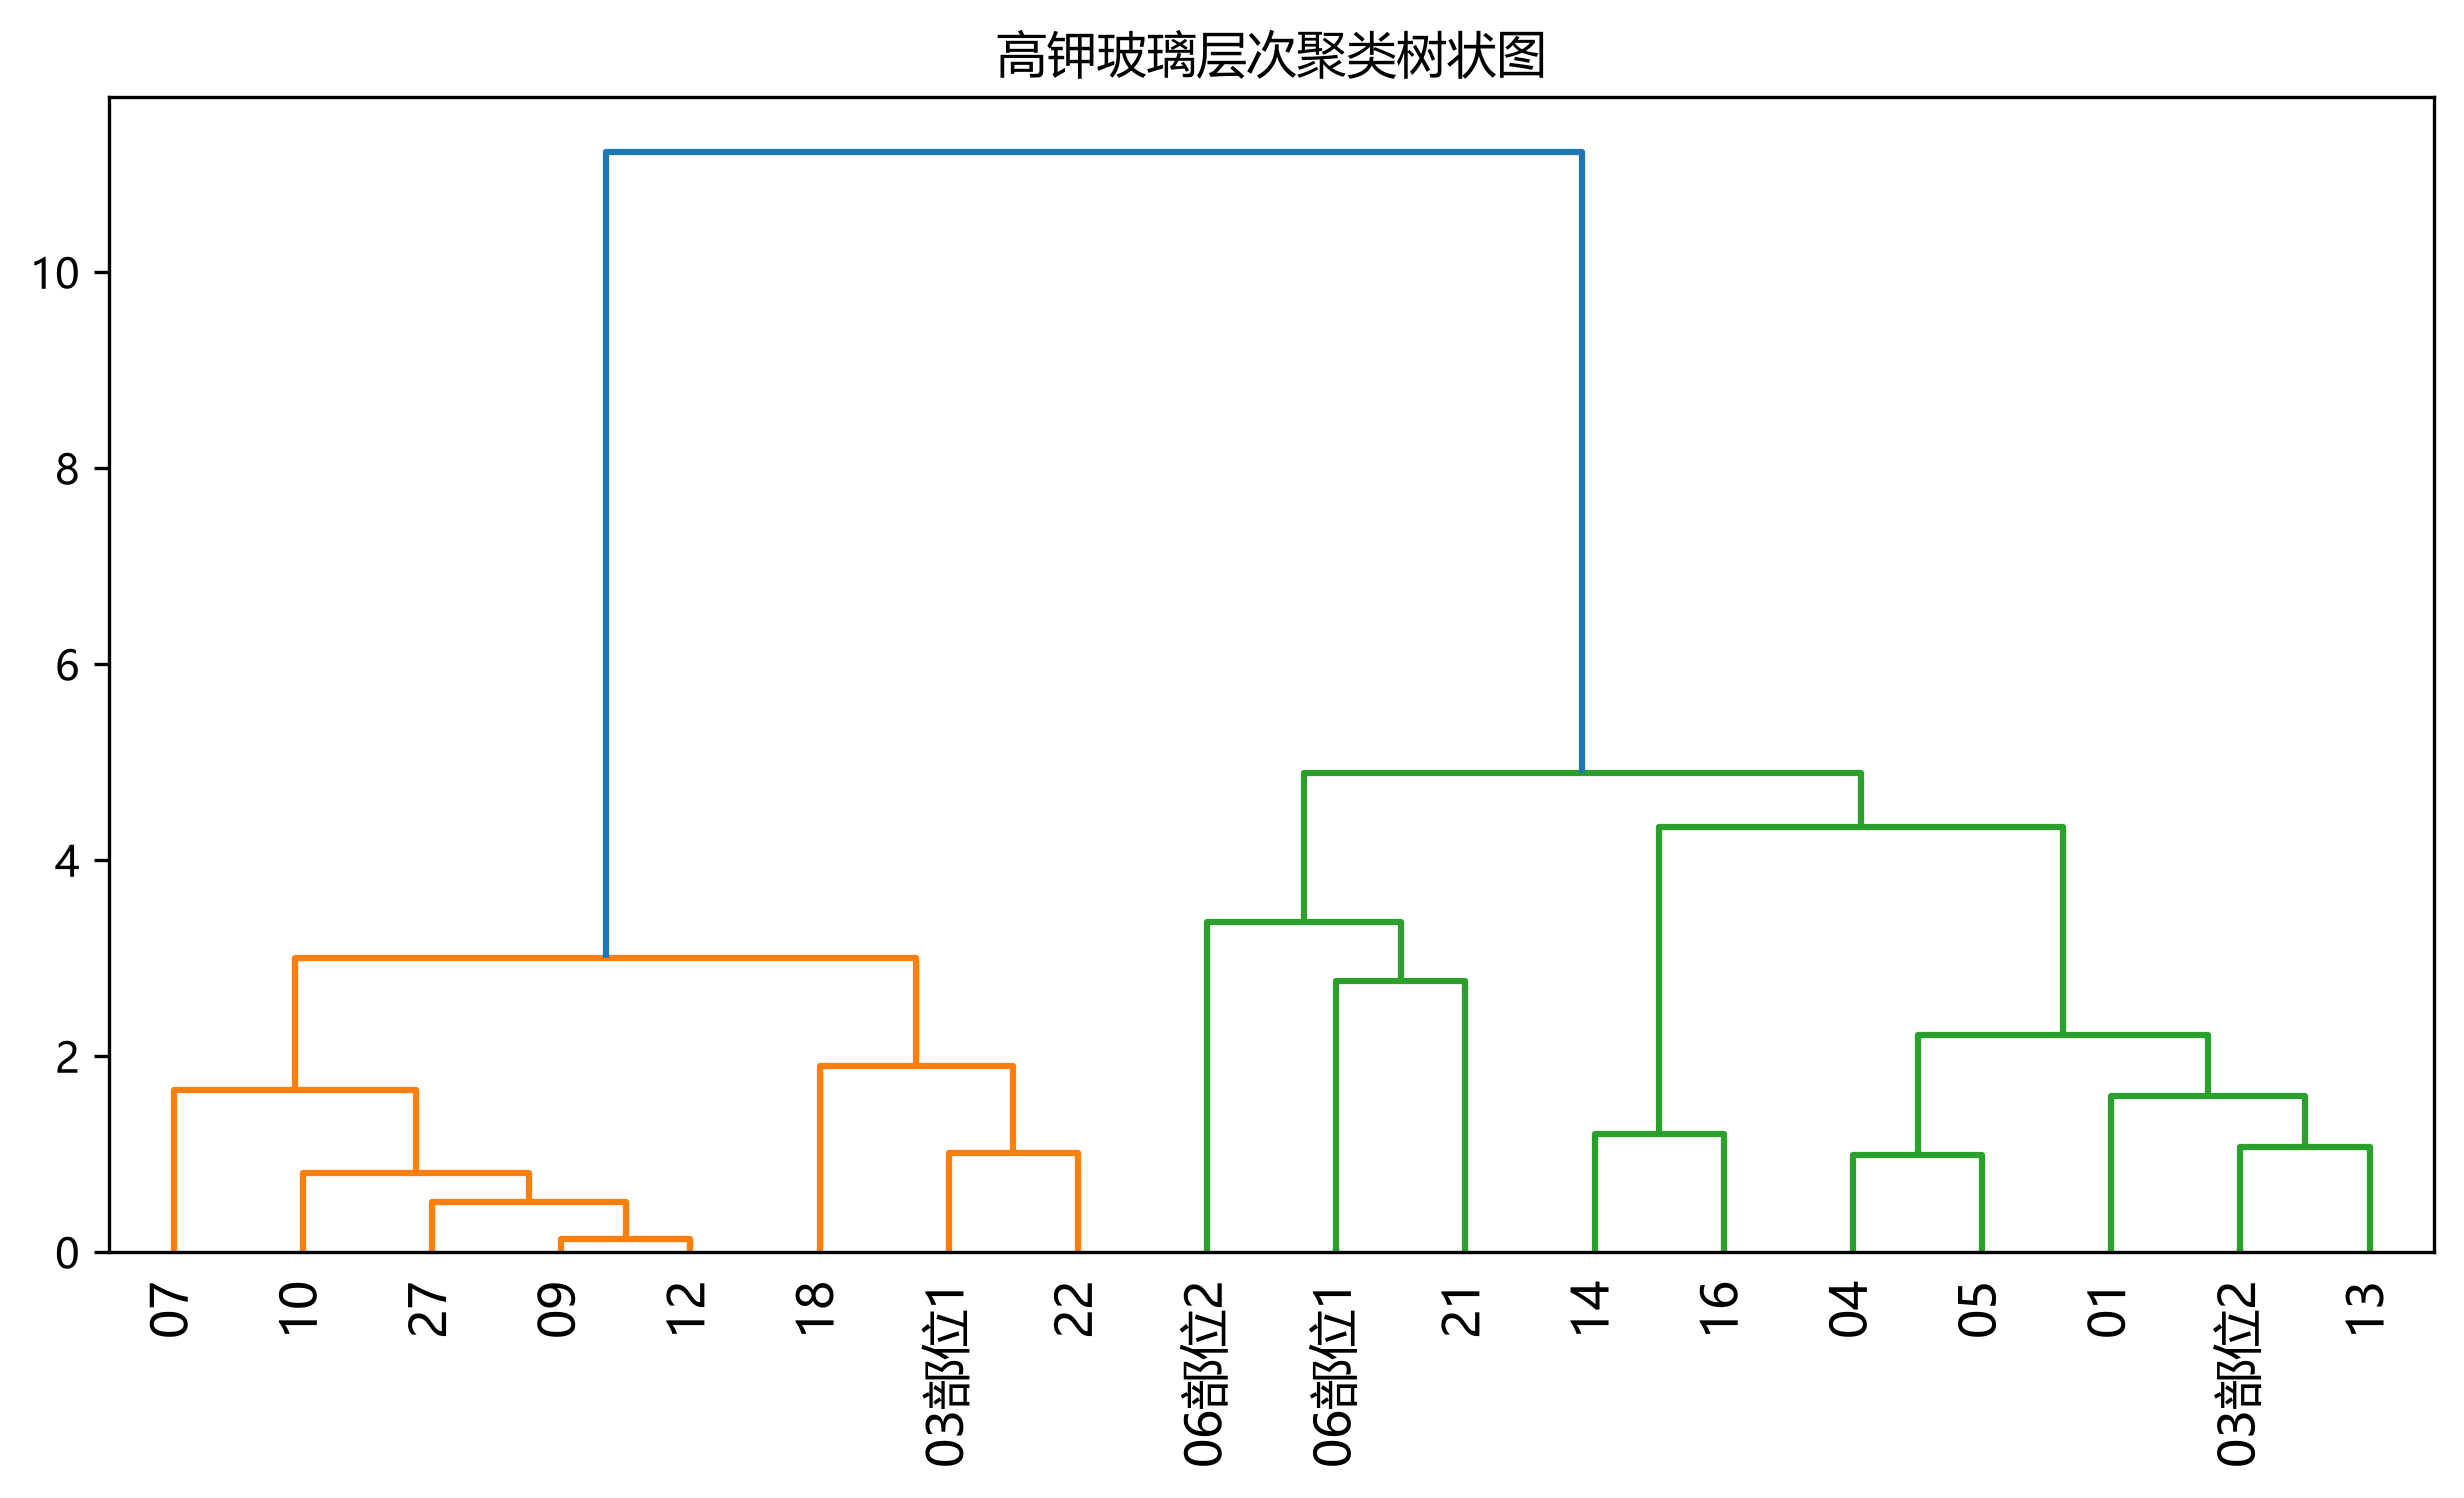
\includegraphics[width=\linewidth]{figures/q2_dendrogram_高钾.png}
\caption{高钾层次聚类树}
\label{fig:dendhk}
\end{minipage}
\hfill
\begin{minipage}{0.48\textwidth}
\centering
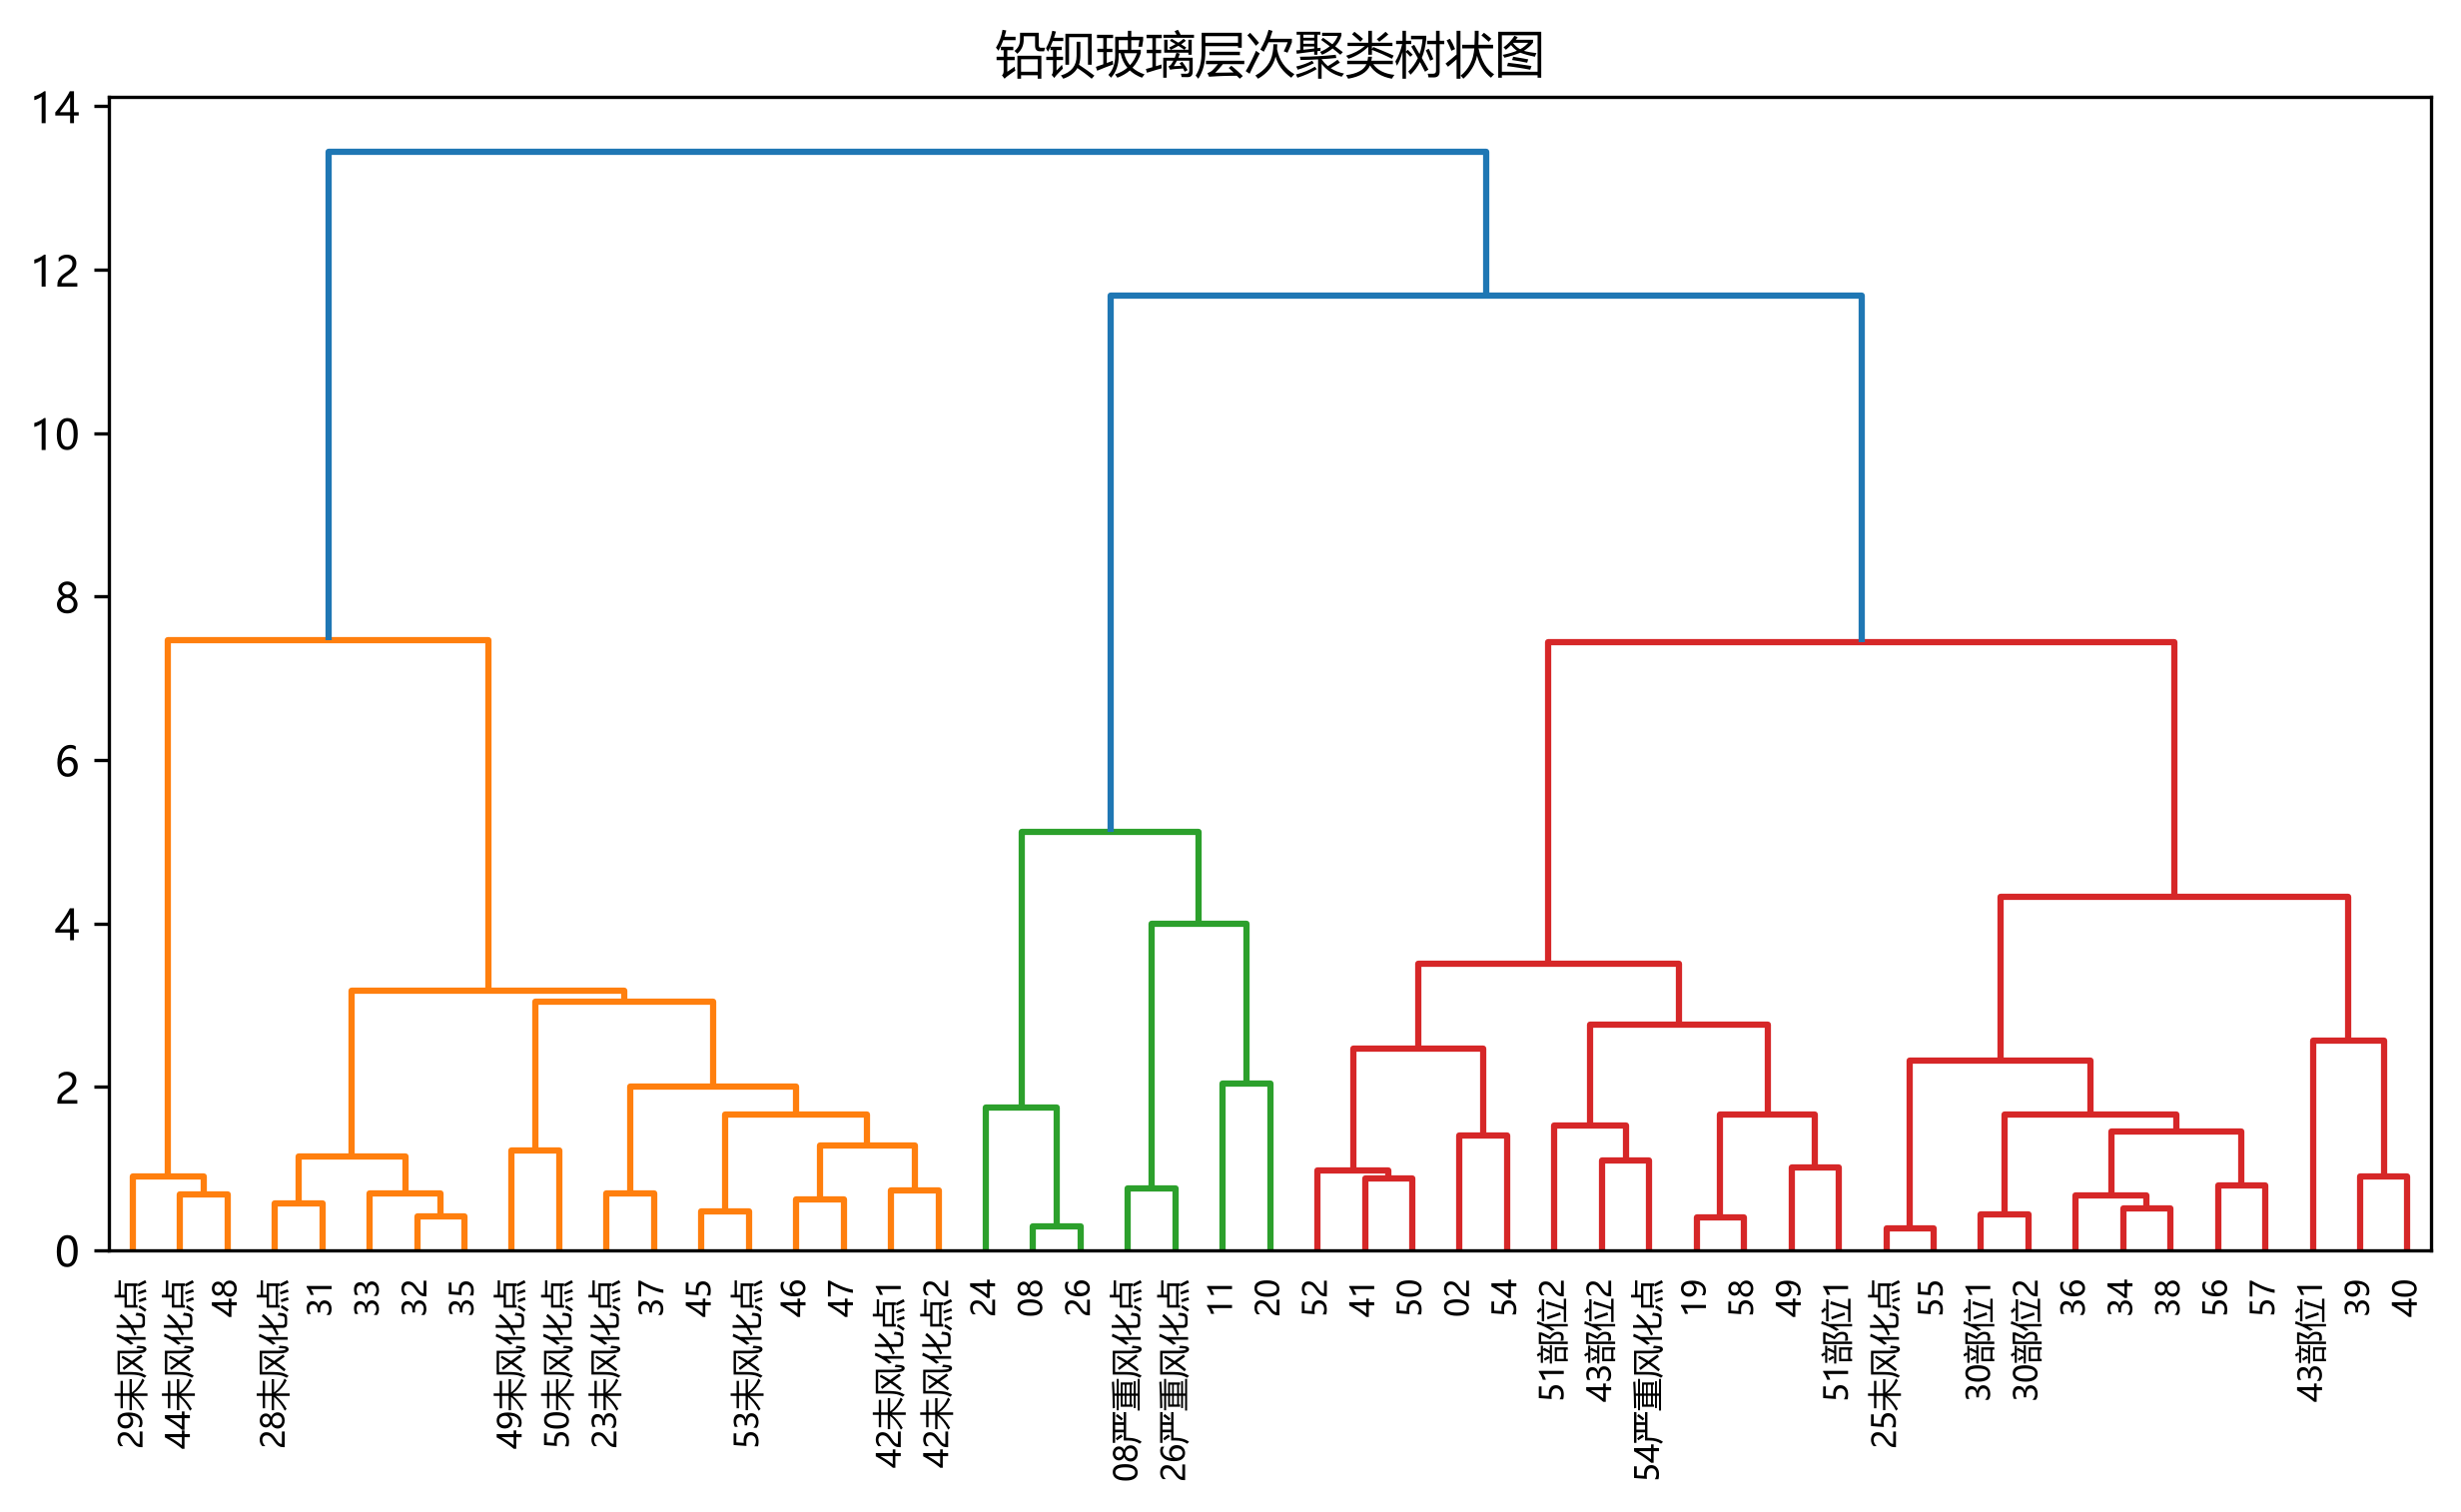
\includegraphics[width=\linewidth]{figures/q2_dendrogram_铅钡.png}
\caption{铅钡层次聚类树}
\label{fig:dendpb}
\end{minipage}
\end{figure}

\subsection{合理性与敏感性}
合理性：亚类中心在SiO$_2$--助熔剂平面上可解释，且轮廓系数显著高于随机标签期望。敏感性：（1）对PbO+BaO规则阈值扫描（图~\ref{fig:thr}）；（2）对成分施加相对噪声$\sigma$，5折准确率从1.0000降至噪声$10\%$时的1.0000（图~\ref{fig:noise}）。

\begin{figure}[H]
\centering
\begin{minipage}{0.48\textwidth}
\centering
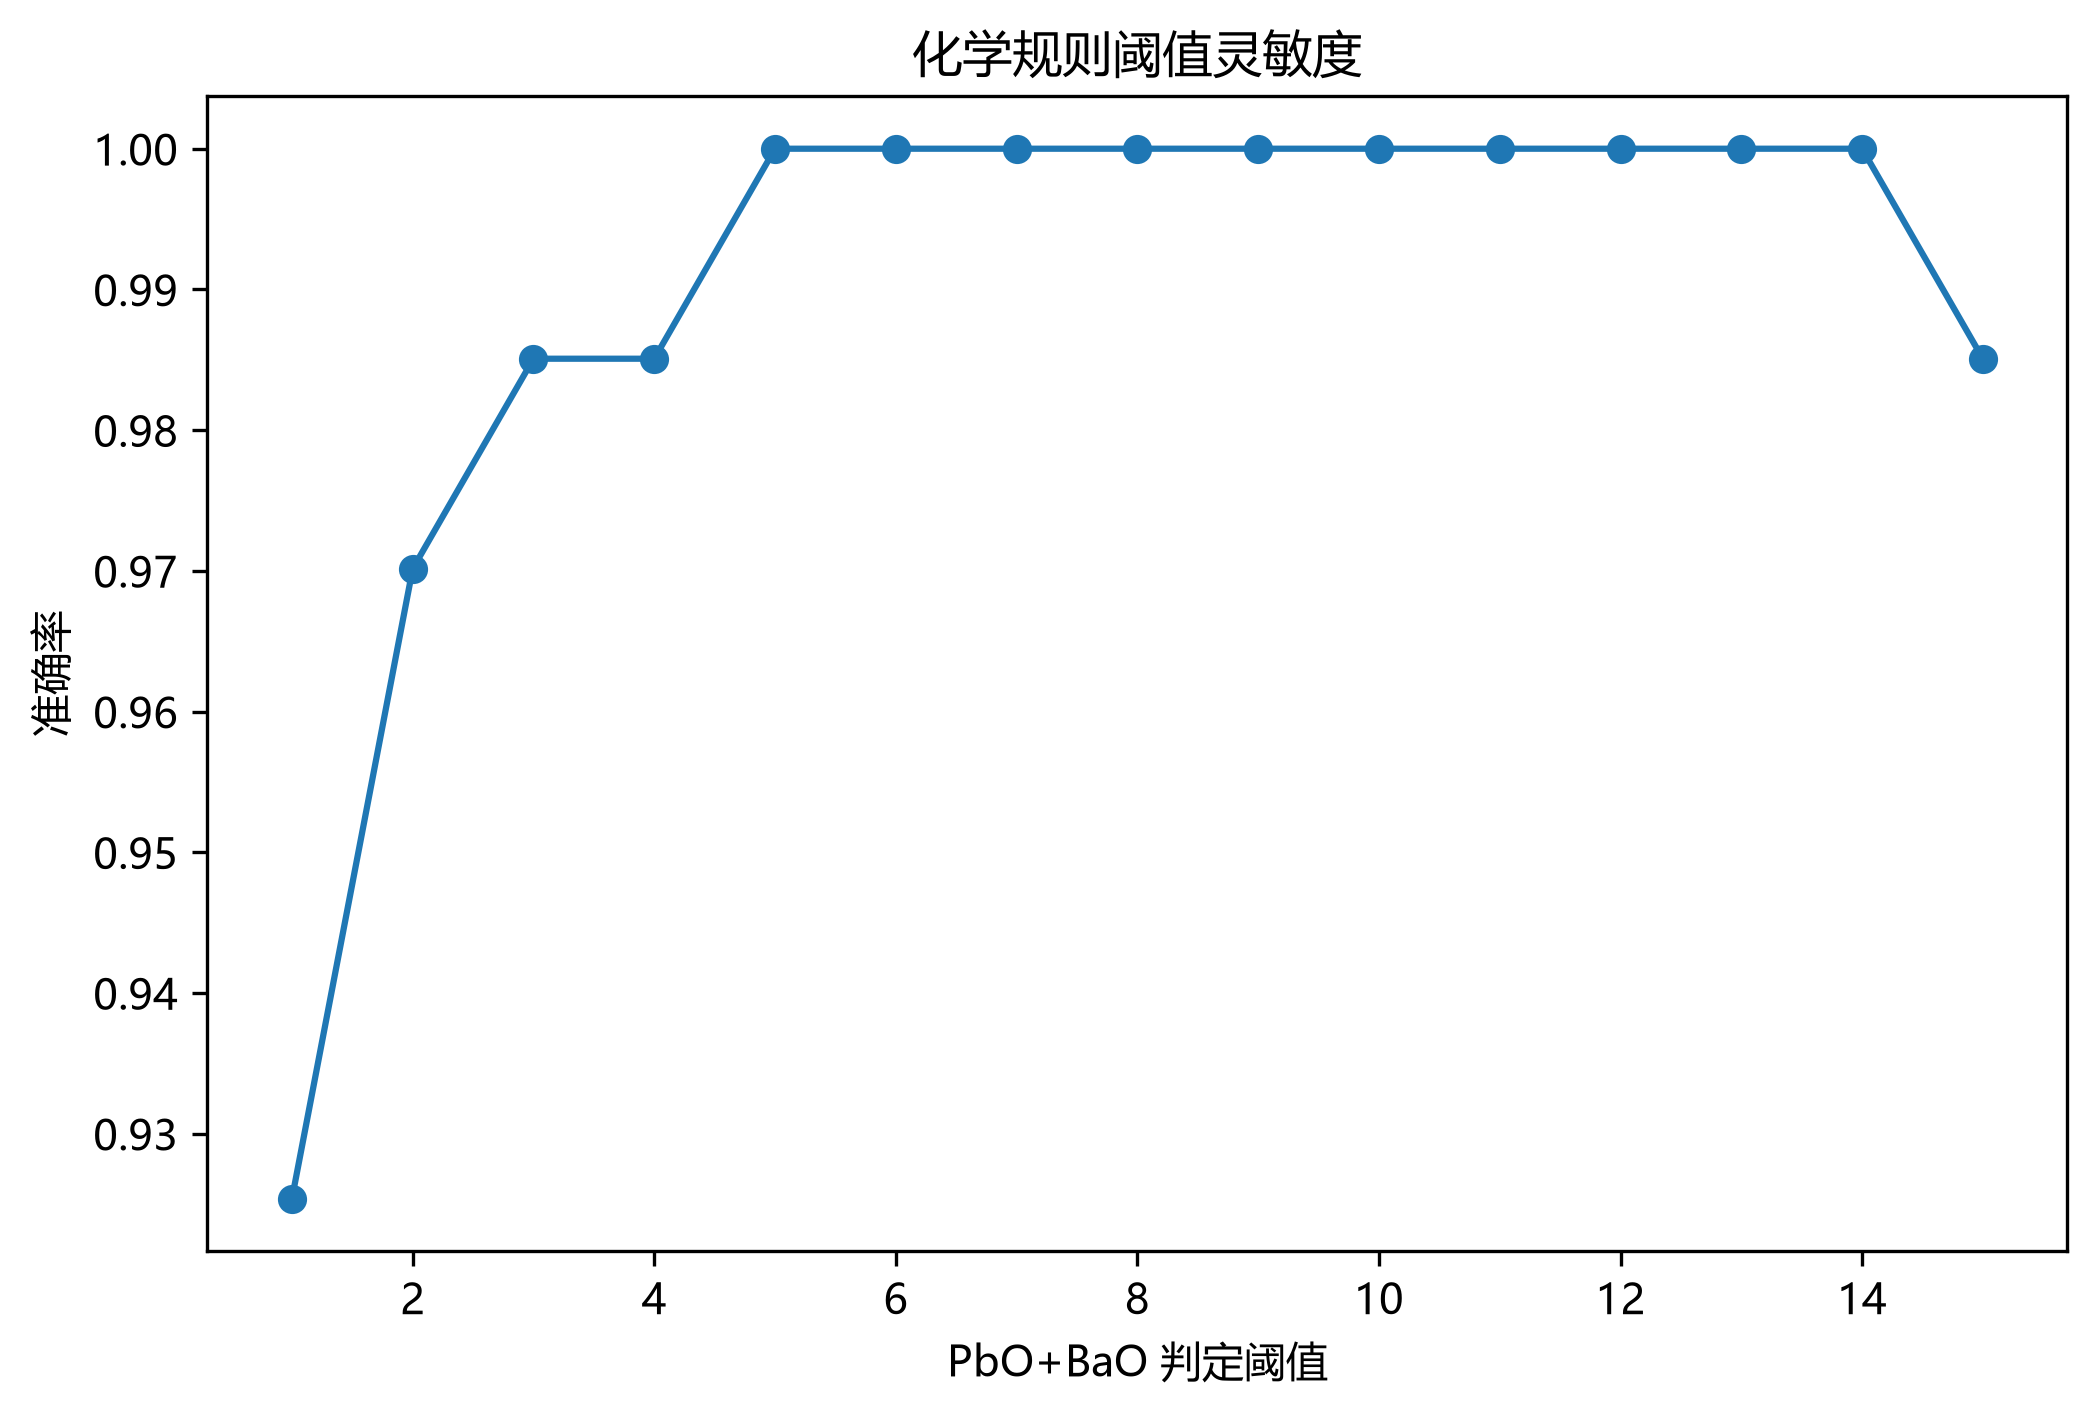
\includegraphics[width=\linewidth]{figures/q2_rule_threshold_sensitivity.png}
\caption{化学规则阈值灵敏度}
\label{fig:thr}
\end{minipage}
\hfill
\begin{minipage}{0.48\textwidth}
\centering
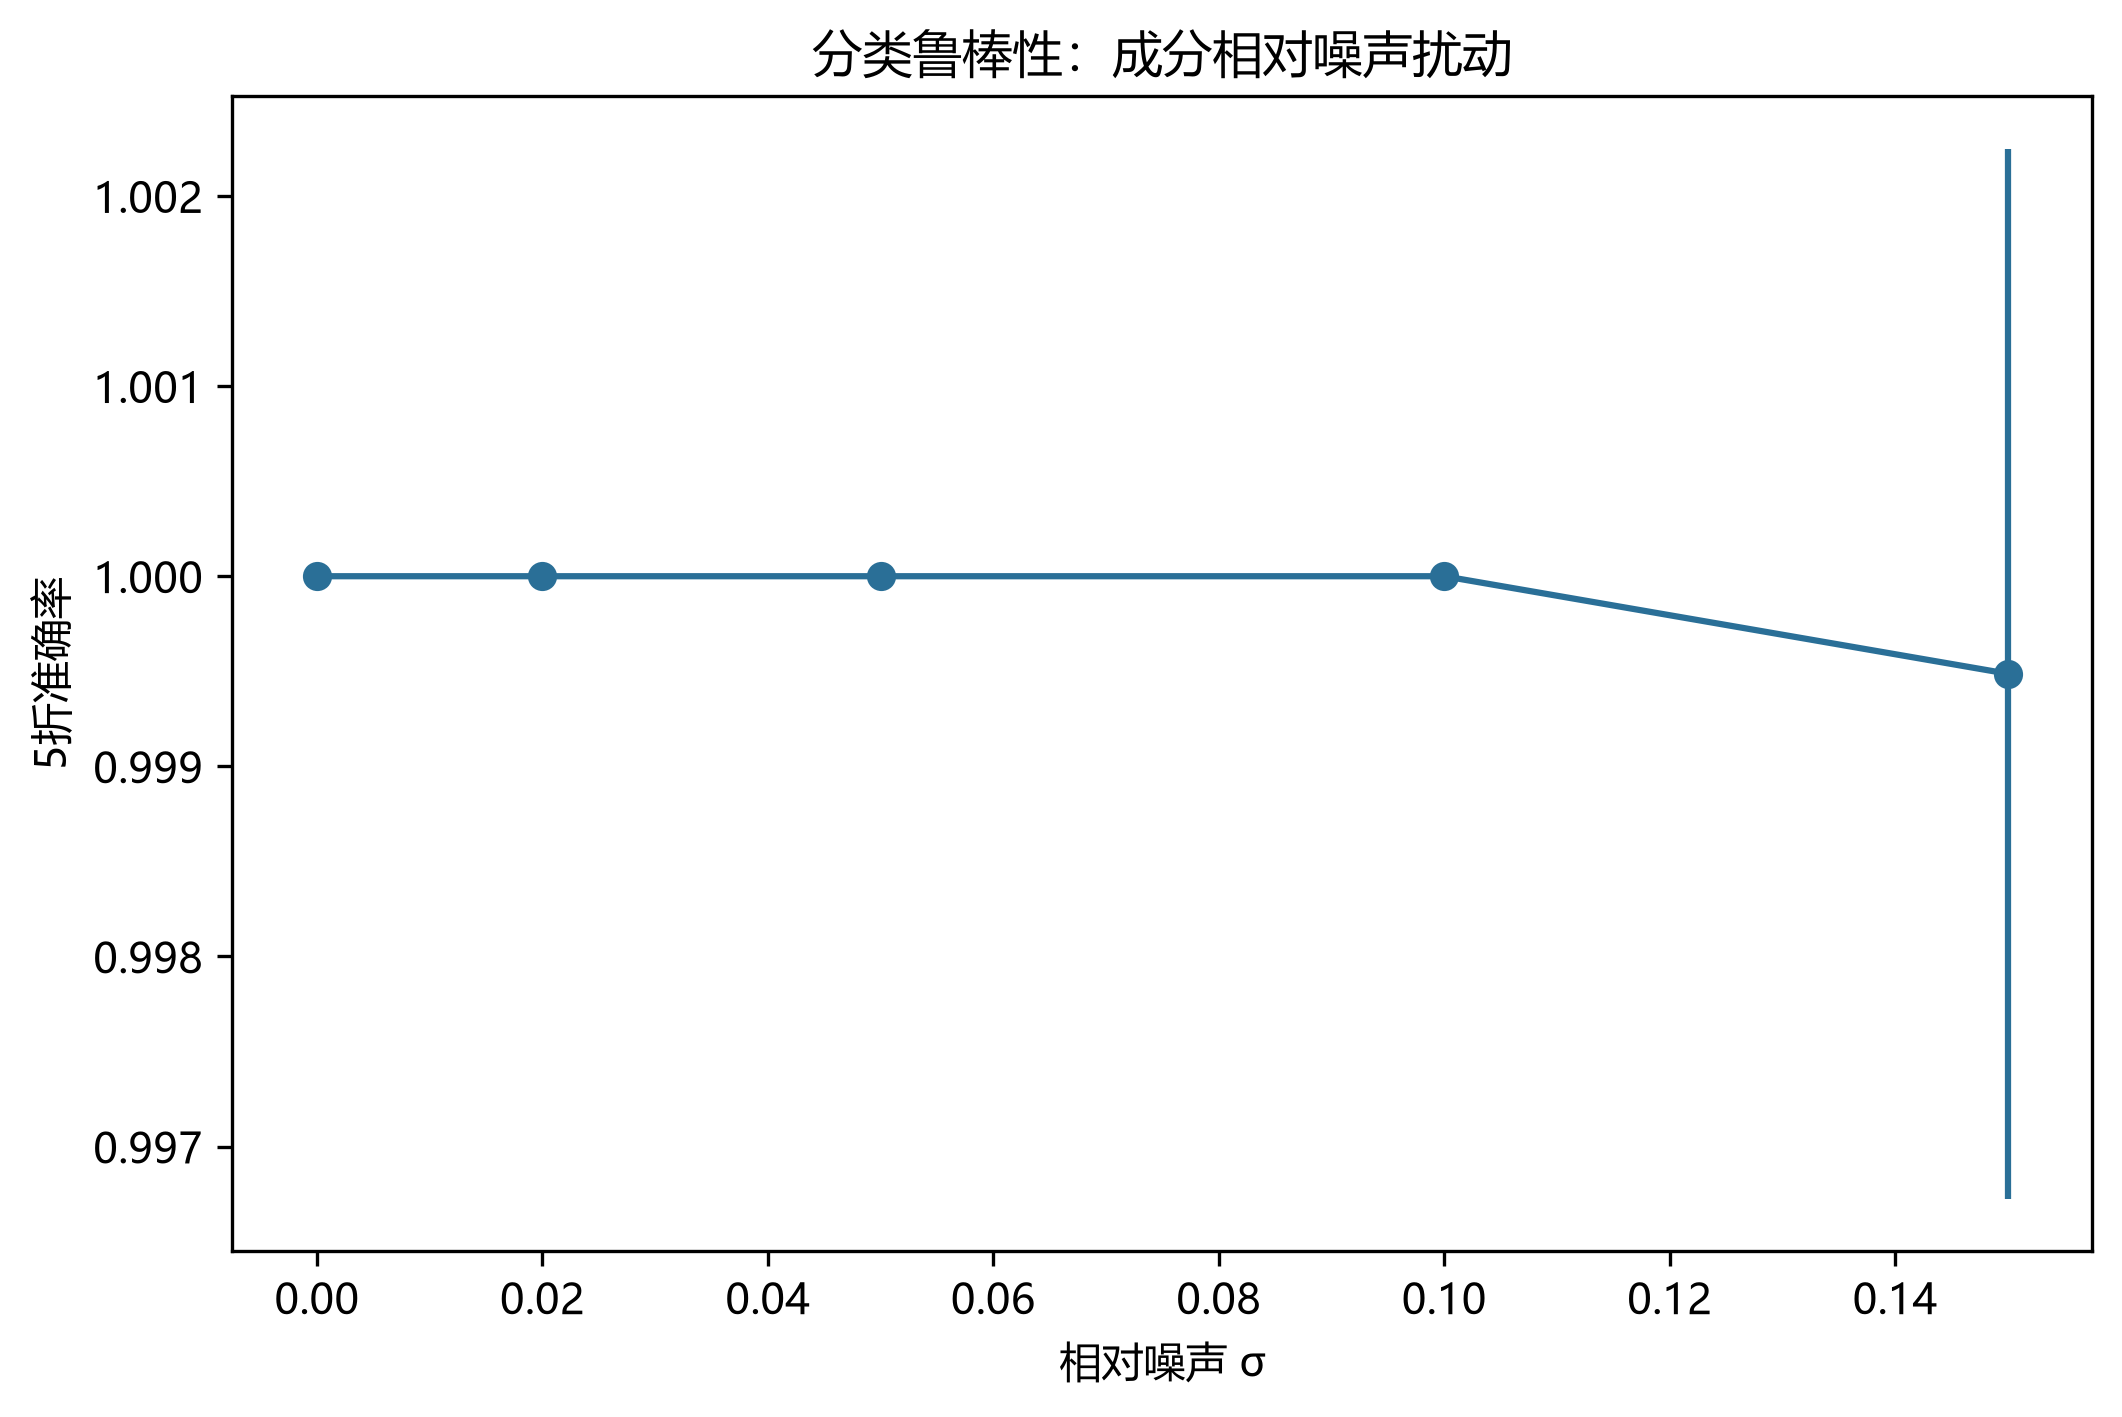
\includegraphics[width=\linewidth]{figures/q2_sensitivity_noise.png}
\caption{分类噪声灵敏度}
\label{fig:noise}
\end{minipage}
\end{figure}

\subsection{与下一问衔接}
将训练好的随机森林概率模型直接用于未知样本，并以噪声翻转率把Q2的灵敏度定义迁移到Q3个体层面。

\section{问题3：未知类别鉴别与敏感性}
\subsection{问题定位}
对表单3样本输出类型标签、置信度与稳定性证据，避免“只给标签不给把握”。

\subsection{鉴别模型}
以随机森林为主模型：
\begin{equation}
\hat{p}_i(y)=\frac{1}{B}\sum_{b=1}^{B} h_b(\mathbf{z}_i)=y,\qquad
\hat{y}_i=\arg\max_y \hat{p}_i(y),\quad
\mathrm{Conf}_i=\max_y\hat{p}_i(y).
\end{equation}
同时给出SVM与化学规则对照。预测结果见表~\ref{tab:pred3}与图~\ref{fig:proba}--\ref{fig:plane}：高钾3件，铅钡5件；RF与SVM一致率1.000，RF与规则一致率1.000，平均置信度0.933。

\begin{table}[H]
\centering
\caption{未知样本鉴别结果}
\label{tab:pred3}
\scriptsize
\begin{tabular}{lcccccccccc}
\toprule
文物编号 & 表面风化 & 规则预测 & RF预测 & SVM预测 & 最终判定 & 置信度 & SiO2 & K2O & PbO & BaO \\
\hline
A1 & 无风化 & 高钾 & 高钾 & 高钾 & 高钾 & 0.917 & 78.450 & 0.000 & 0.000 & 0.000 \\
A2 & 风化 & 铅钡 & 铅钡 & 铅钡 & 铅钡 & 0.900 & 37.750 & 0.000 & 34.300 & 0.000 \\
A3 & 无风化 & 铅钡 & 铅钡 & 铅钡 & 铅钡 & 0.890 & 31.950 & 1.360 & 39.580 & 4.690 \\
A4 & 无风化 & 铅钡 & 铅钡 & 铅钡 & 铅钡 & 0.937 & 35.470 & 0.790 & 24.280 & 8.310 \\
A5 & 风化 & 铅钡 & 铅钡 & 铅钡 & 铅钡 & 0.840 & 64.290 & 0.370 & 12.230 & 2.160 \\
A6 & 风化 & 高钾 & 高钾 & 高钾 & 高钾 & 1.000 & 93.170 & 1.350 & 0.000 & 0.000 \\
A7 & 风化 & 高钾 & 高钾 & 高钾 & 高钾 & 0.983 & 90.830 & 0.980 & 0.000 & 0.000 \\
A8 & 无风化 & 铅钡 & 铅钡 & 铅钡 & 铅钡 & 1.000 & 51.120 & 0.230 & 21.240 & 11.340 \\
\bottomrule
\end{tabular}
\end{table}

\begin{figure}[H]
\centering
\begin{minipage}{0.48\textwidth}
\centering
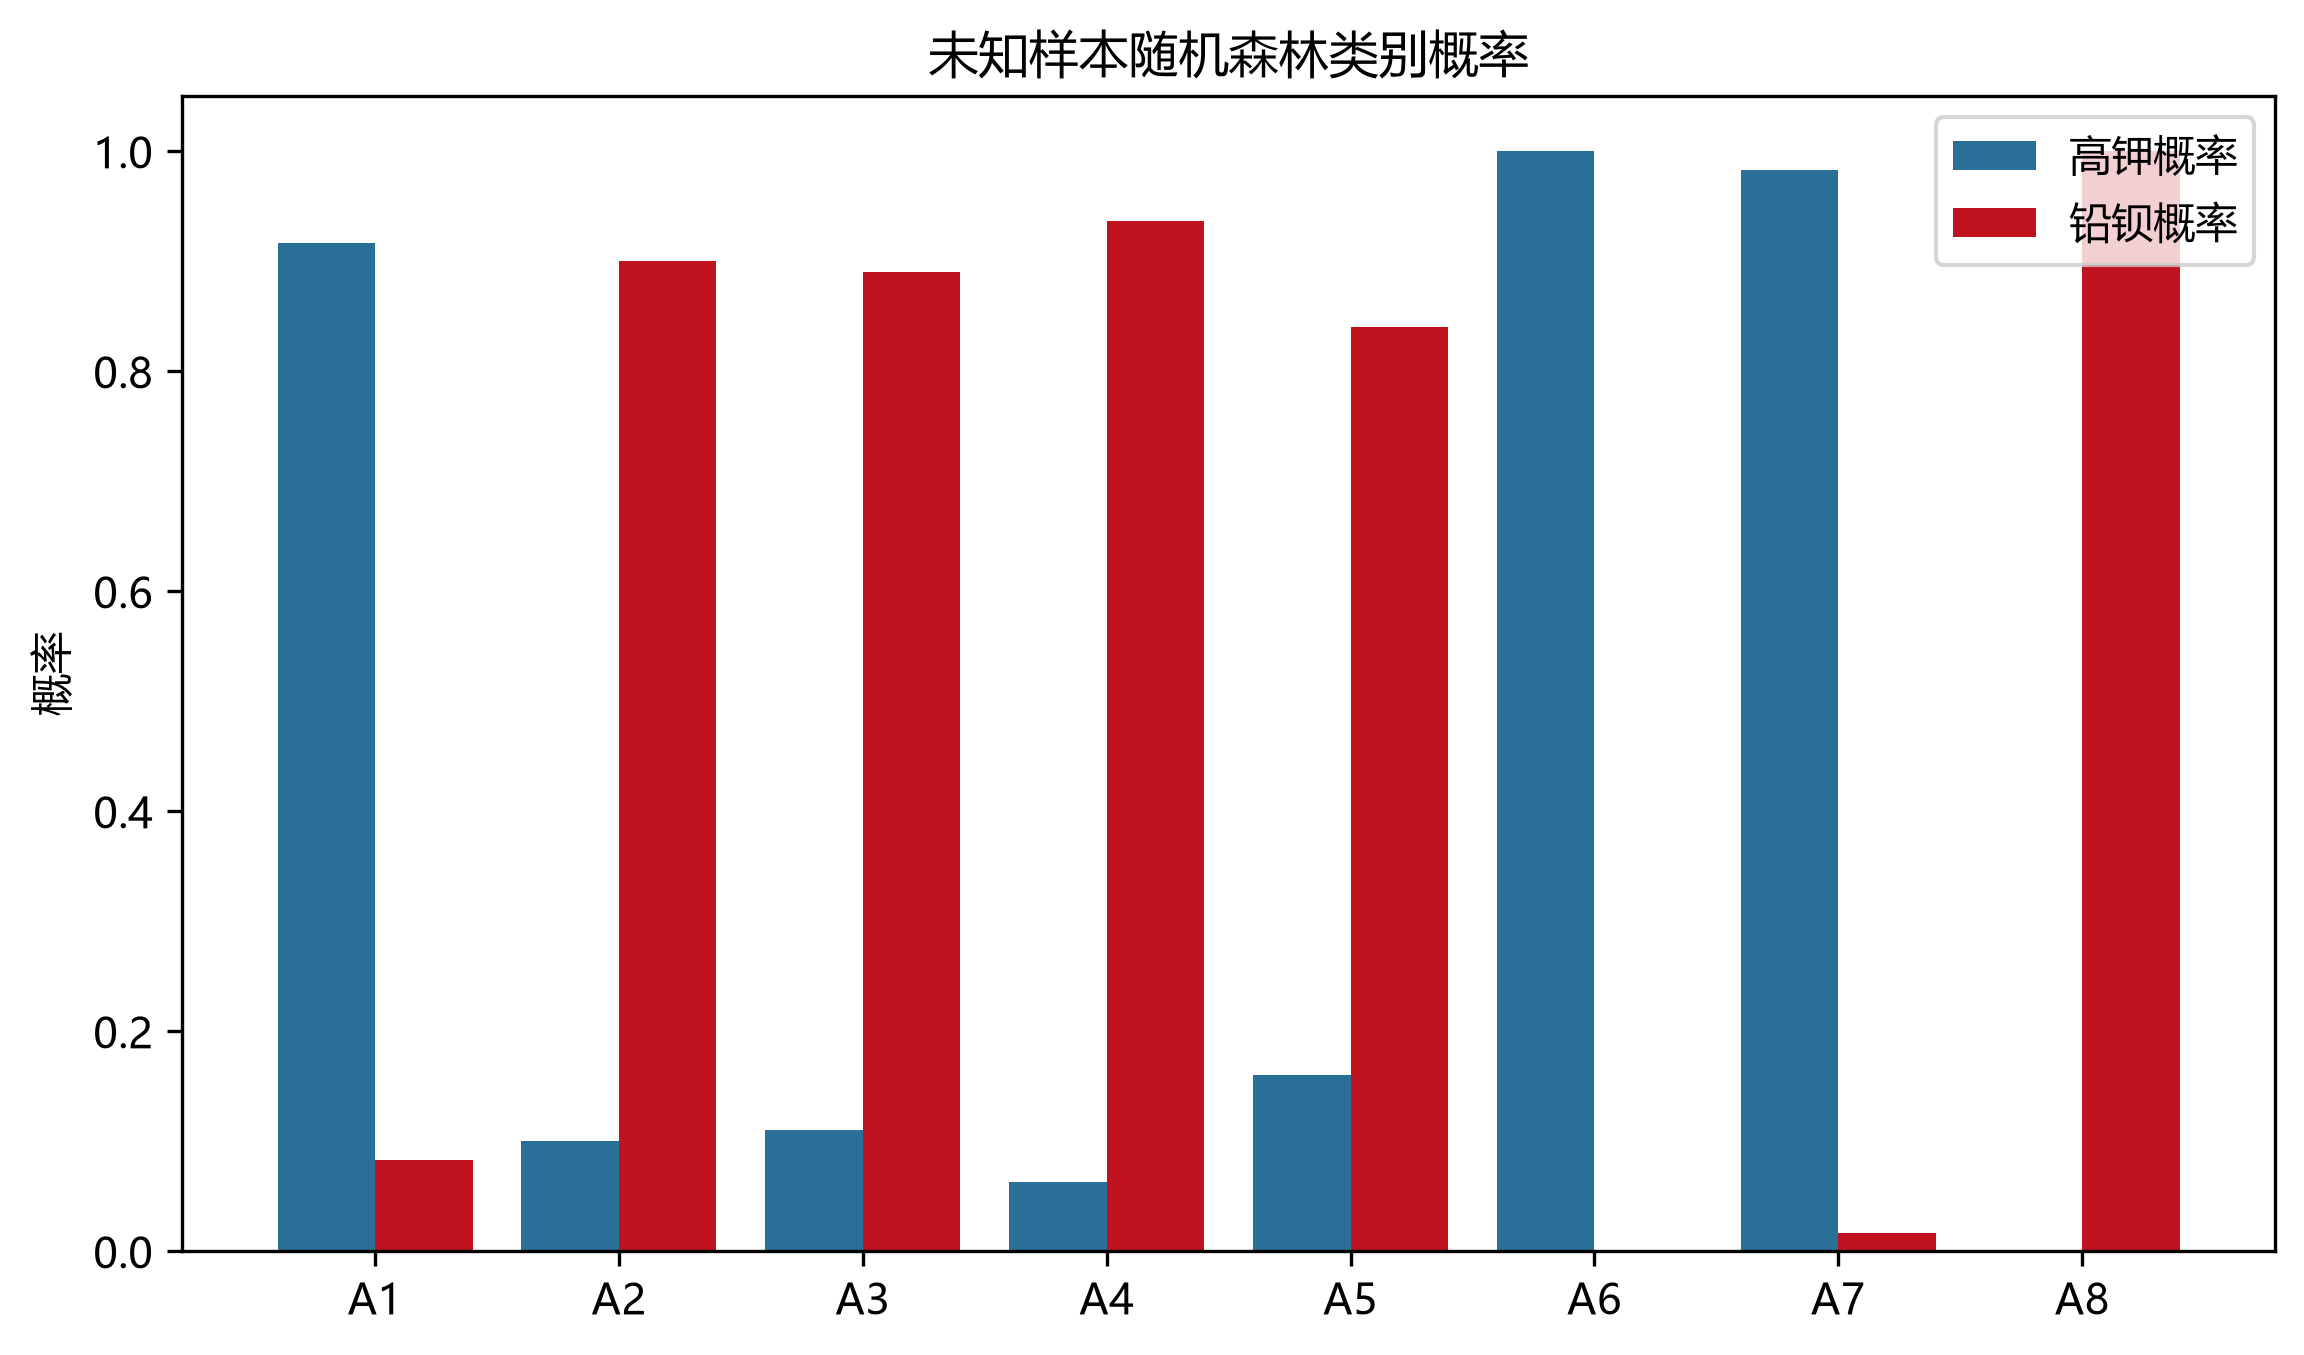
\includegraphics[width=\linewidth]{figures/q3_rf_proba.png}
\caption{未知样本类别概率}
\label{fig:proba}
\end{minipage}
\hfill
\begin{minipage}{0.48\textwidth}
\centering
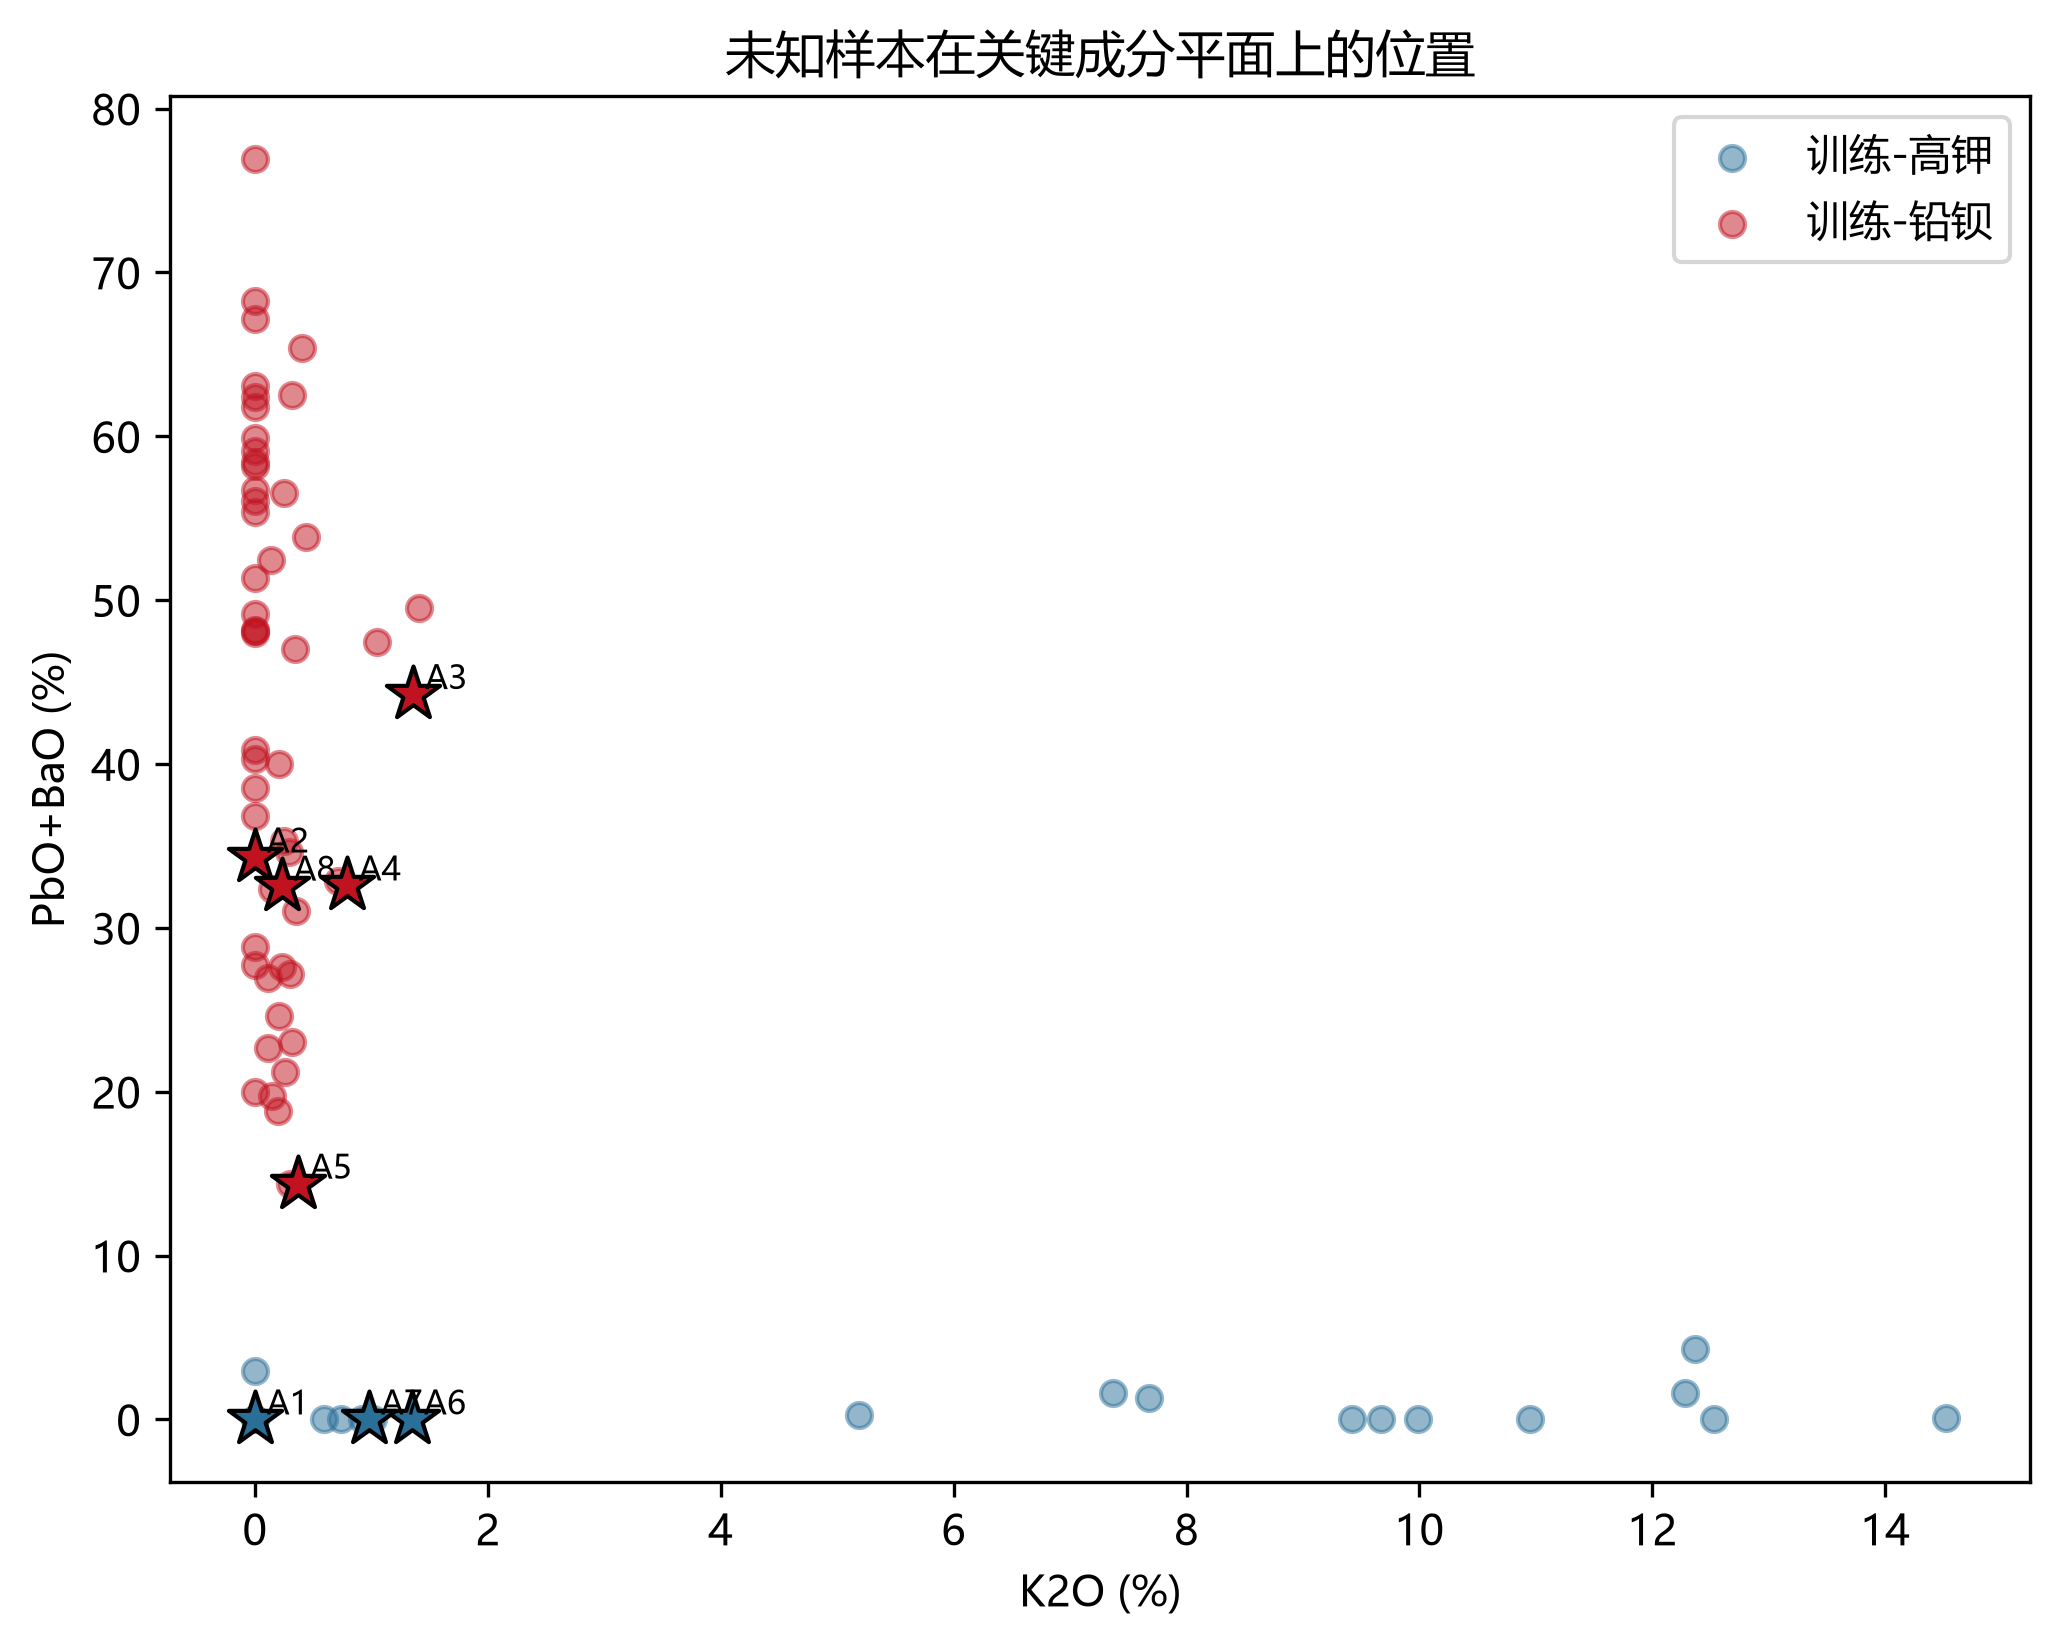
\includegraphics[width=\linewidth]{figures/q3_feature_plane.png}
\caption{未知样本在K$_2$O--(PbO+BaO)平面位置}
\label{fig:plane}
\end{minipage}
\end{figure}

\subsection{敏感性分析}
对测试成分施加$5\%$相对高斯噪声并重复$100$次，定义翻转率
\begin{equation}
\mathrm{Flip}_i=\frac{1}{M}\sum_{m=1}^{M}\mathbf{1}(\hat{y}_i^{(m)}\ne \hat{y}_i).
\end{equation}
另在训练集上做留一删除，统计未知样本标签稳定比例。结果见表~\ref{tab:flip}与图~\ref{fig:flip}：平均翻转率0.000，平均稳定比例1.000。

\begin{table}[H]
\centering
\caption{未知样本噪声翻转率}
\label{tab:flip}
\scriptsize
\begin{tabular}{lcccc}
\toprule
文物编号 & 最终判定 & 置信度 & 翻转次数 & 翻转率 \\
\hline
A1 & 高钾 & 0.917 & 0 & 0.000 \\
A2 & 铅钡 & 0.900 & 0 & 0.000 \\
A3 & 铅钡 & 0.890 & 0 & 0.000 \\
A4 & 铅钡 & 0.937 & 0 & 0.000 \\
A5 & 铅钡 & 0.840 & 0 & 0.000 \\
A6 & 高钾 & 1.000 & 0 & 0.000 \\
A7 & 高钾 & 0.983 & 0 & 0.000 \\
A8 & 铅钡 & 1.000 & 0 & 0.000 \\
\bottomrule
\end{tabular}
\end{table}

\begin{figure}[H]
\centering
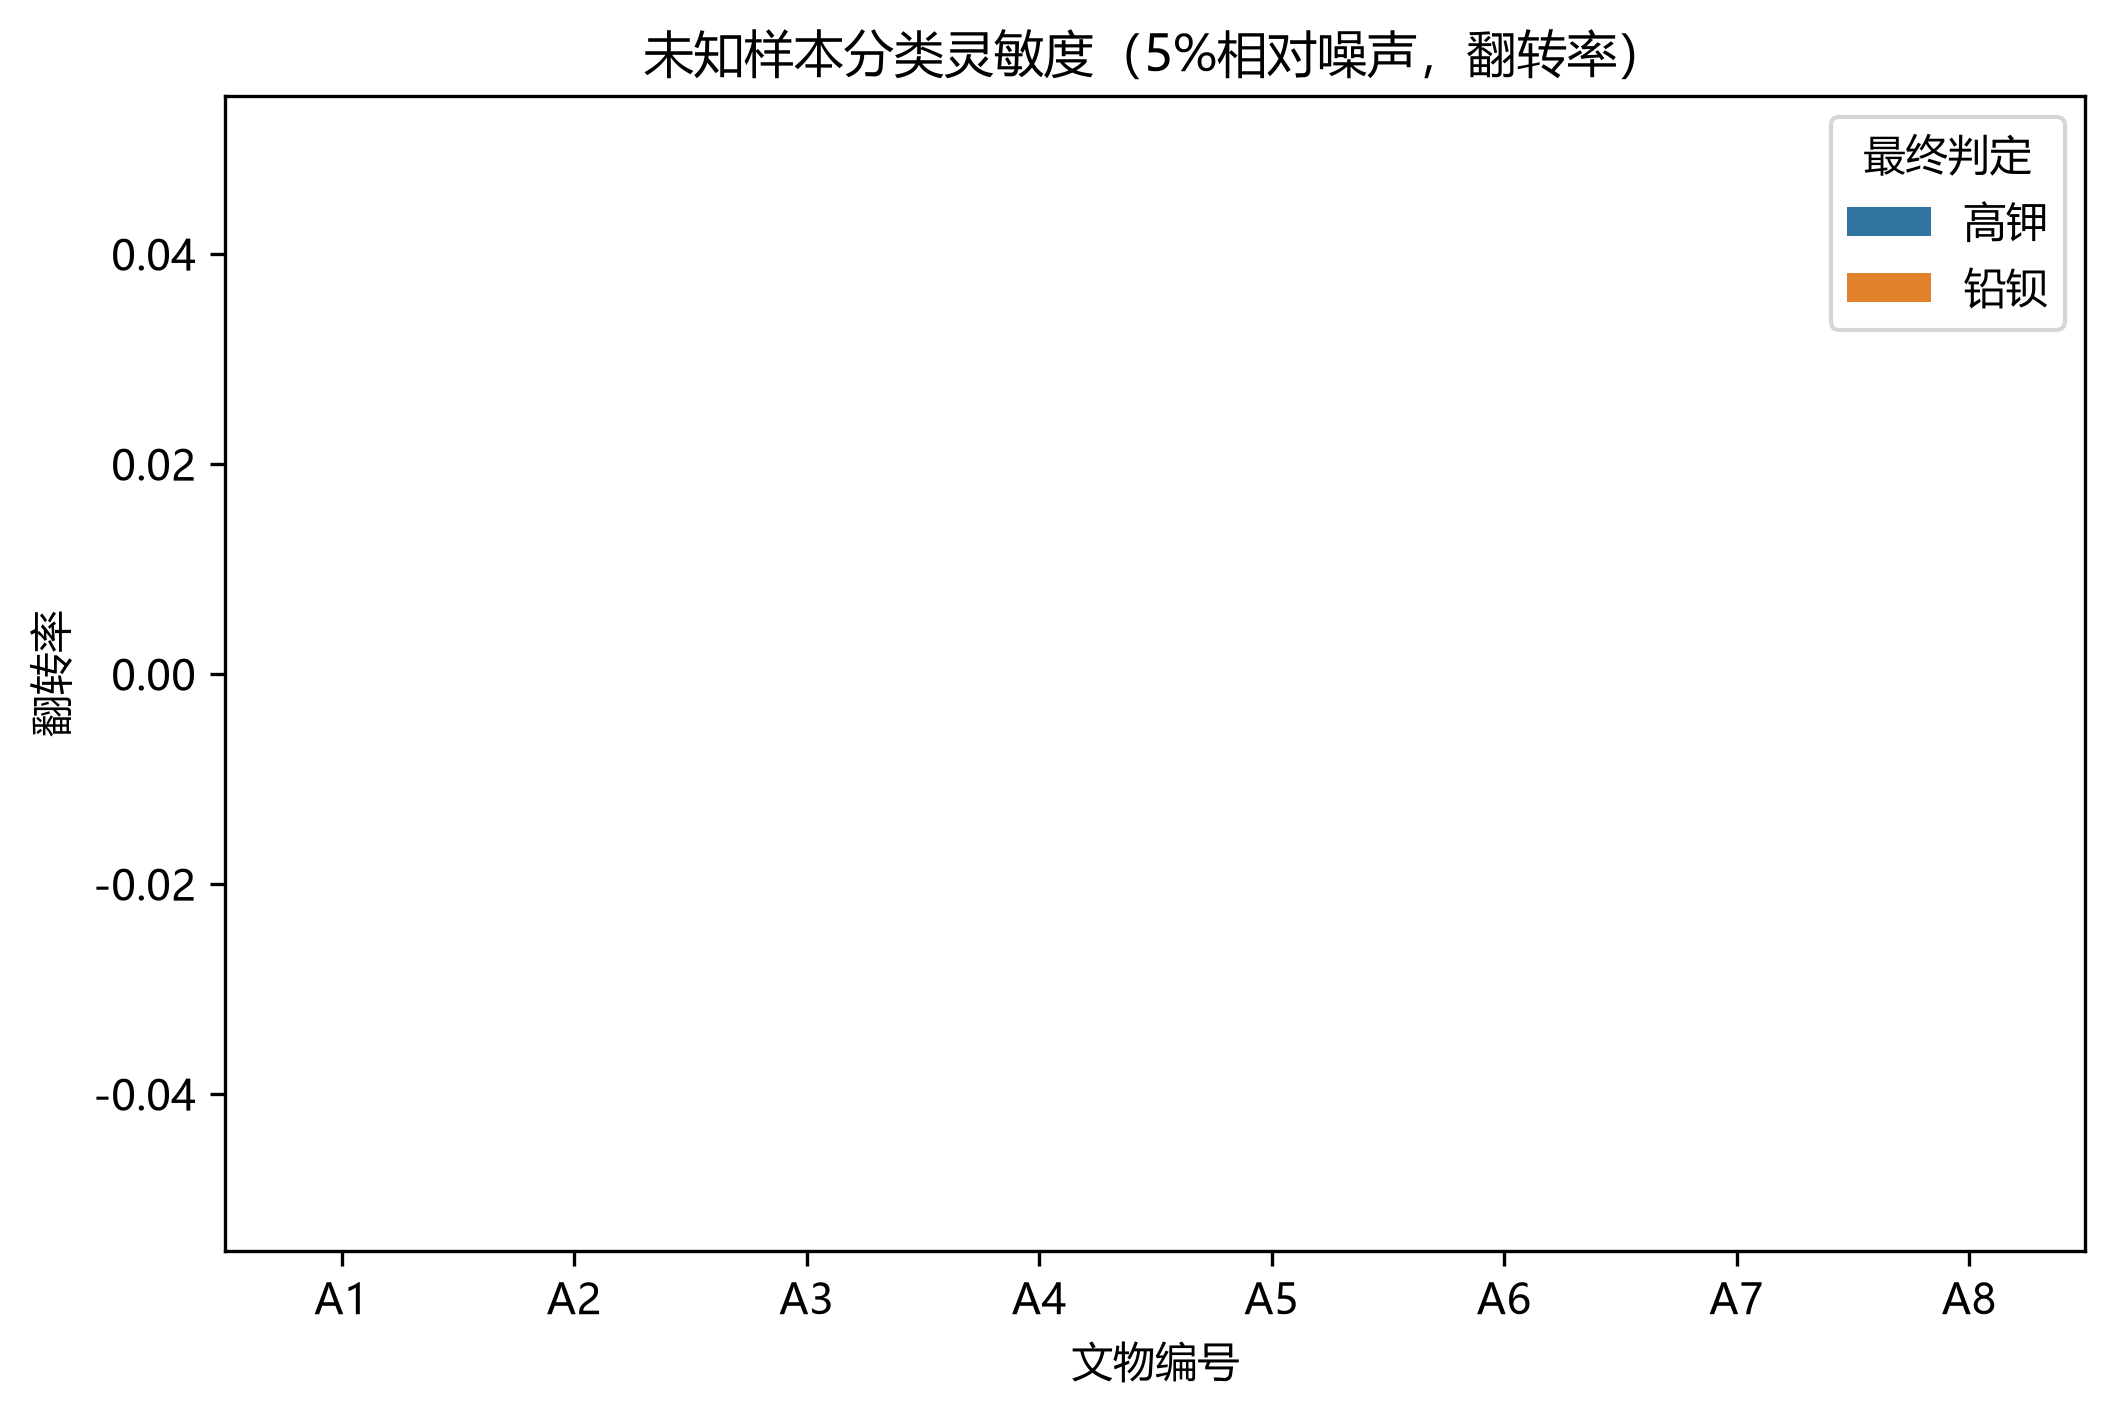
\includegraphics[width=0.75\textwidth]{figures/q3_flip_rate.png}
\caption{未知样本分类翻转率}
\label{fig:flip}
\end{figure}

\section{问题4：成分关联关系及其类别差异}
\subsection{问题定位}
从“成对相关结构”解释两类玻璃的配方约束差异，而不是只比较单成分均值。

\subsection{相关模型}
对类型$t$计算Spearman秩相关
\begin{equation}
r_{ab}^{(t)}=1-\frac{6\sum_i d_{i,ab}^2}{n_t(n_t^2-1)},
\end{equation}
并在$|r|\ge0.5$且$p<0.05$时连边构建相关网络。高钾显著相关对32，铅钡40。热力图与网络见图~\ref{fig:hmhk}--\ref{fig:netpb}。

\begin{figure}[H]
\centering
\begin{minipage}{0.48\textwidth}
\centering
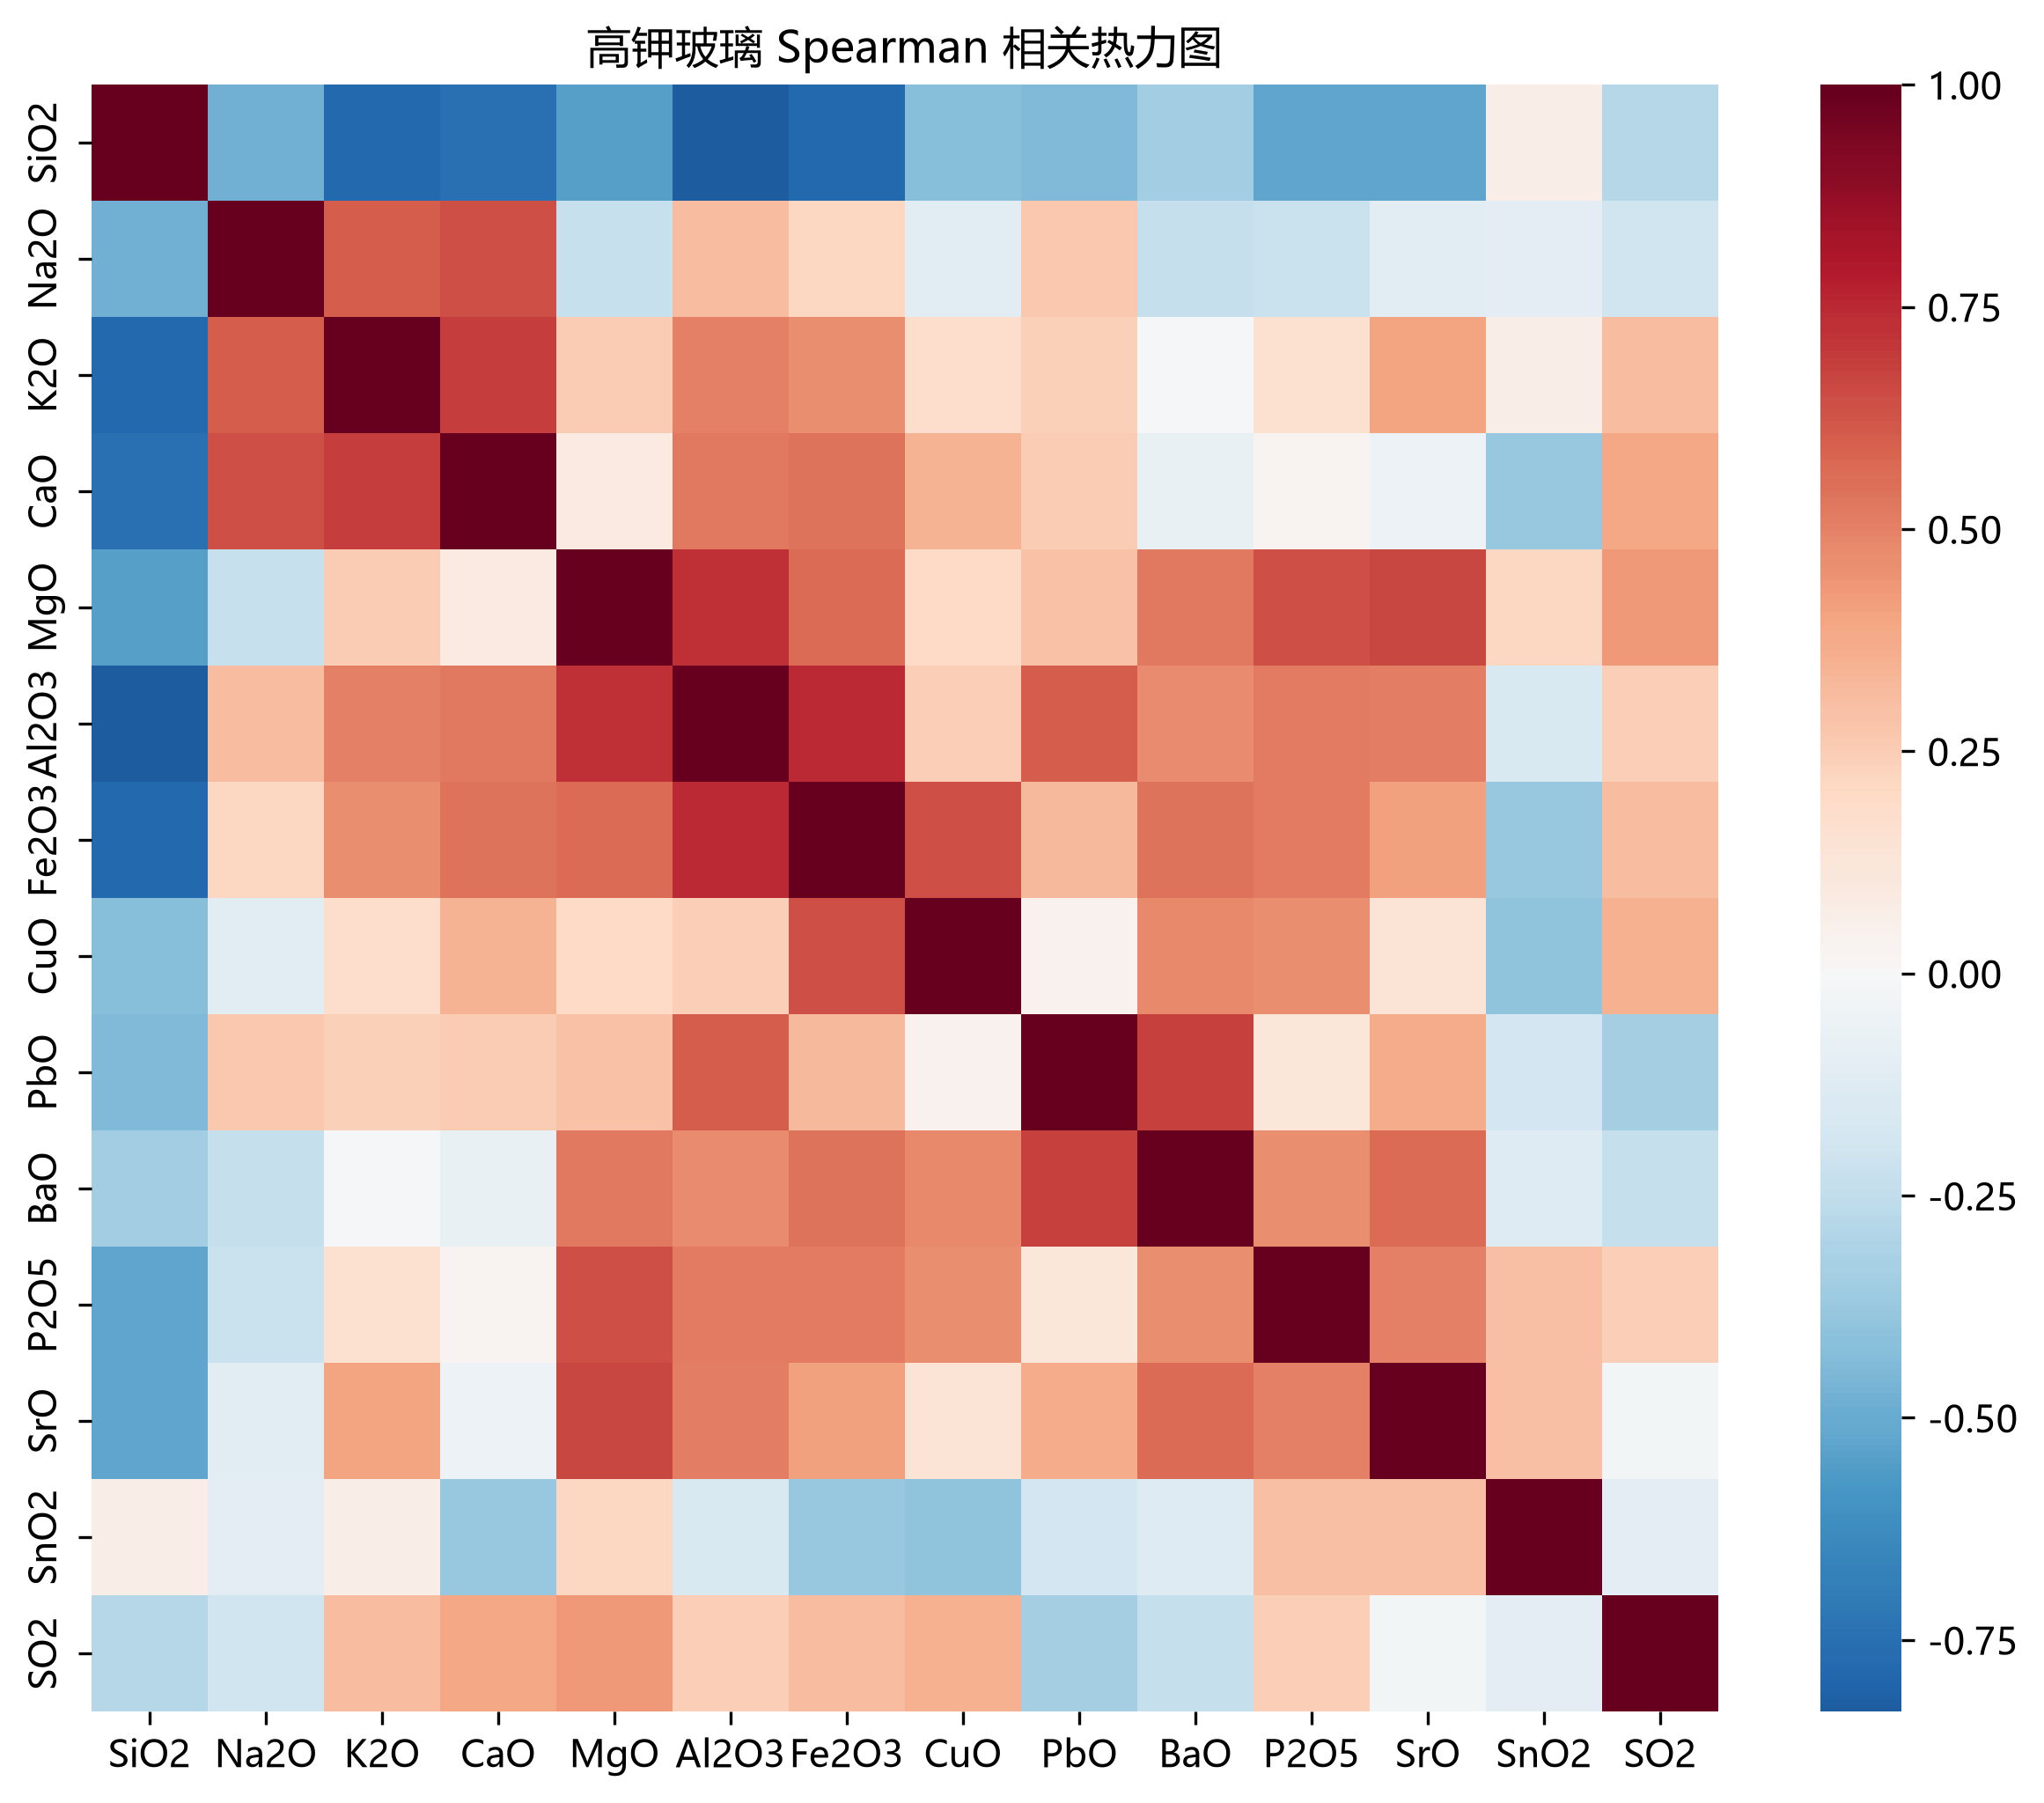
\includegraphics[width=\linewidth]{figures/q4_heatmap_高钾.png}
\caption{高钾Spearman热力图}
\label{fig:hmhk}
\end{minipage}
\hfill
\begin{minipage}{0.48\textwidth}
\centering
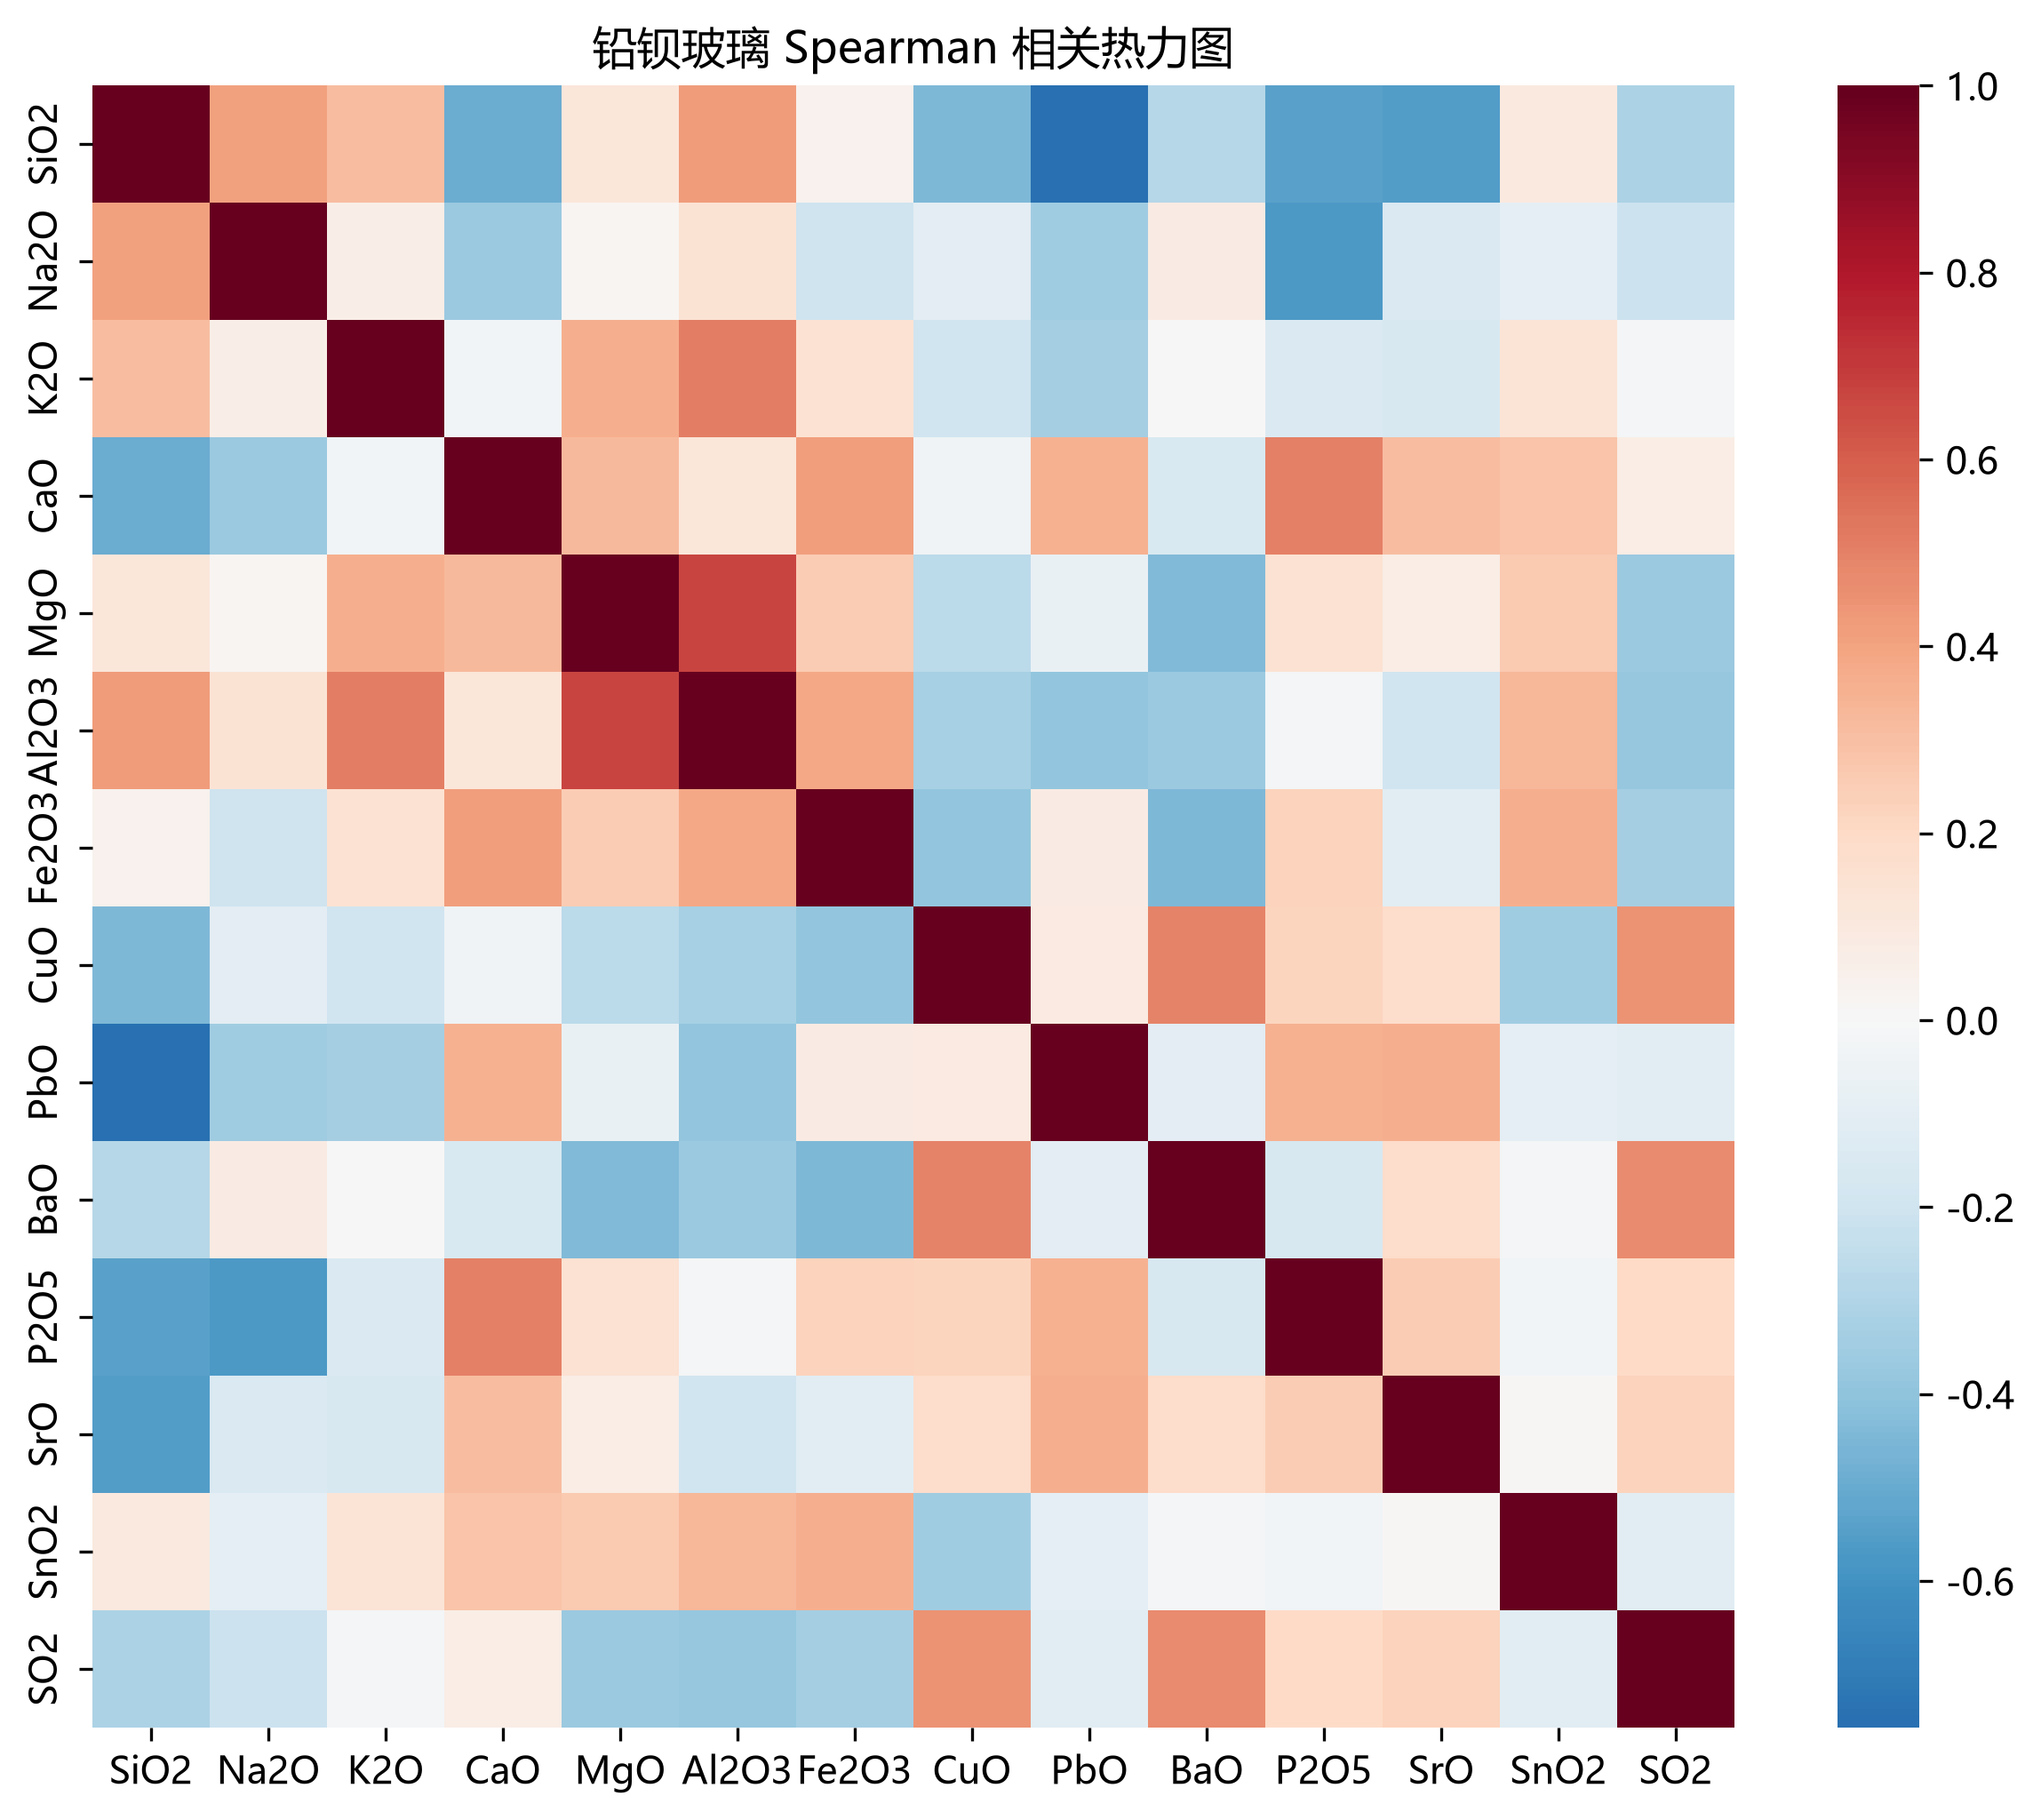
\includegraphics[width=\linewidth]{figures/q4_heatmap_铅钡.png}
\caption{铅钡Spearman热力图}
\label{fig:hmpb}
\end{minipage}
\end{figure}

\begin{figure}[H]
\centering
\begin{minipage}{0.48\textwidth}
\centering
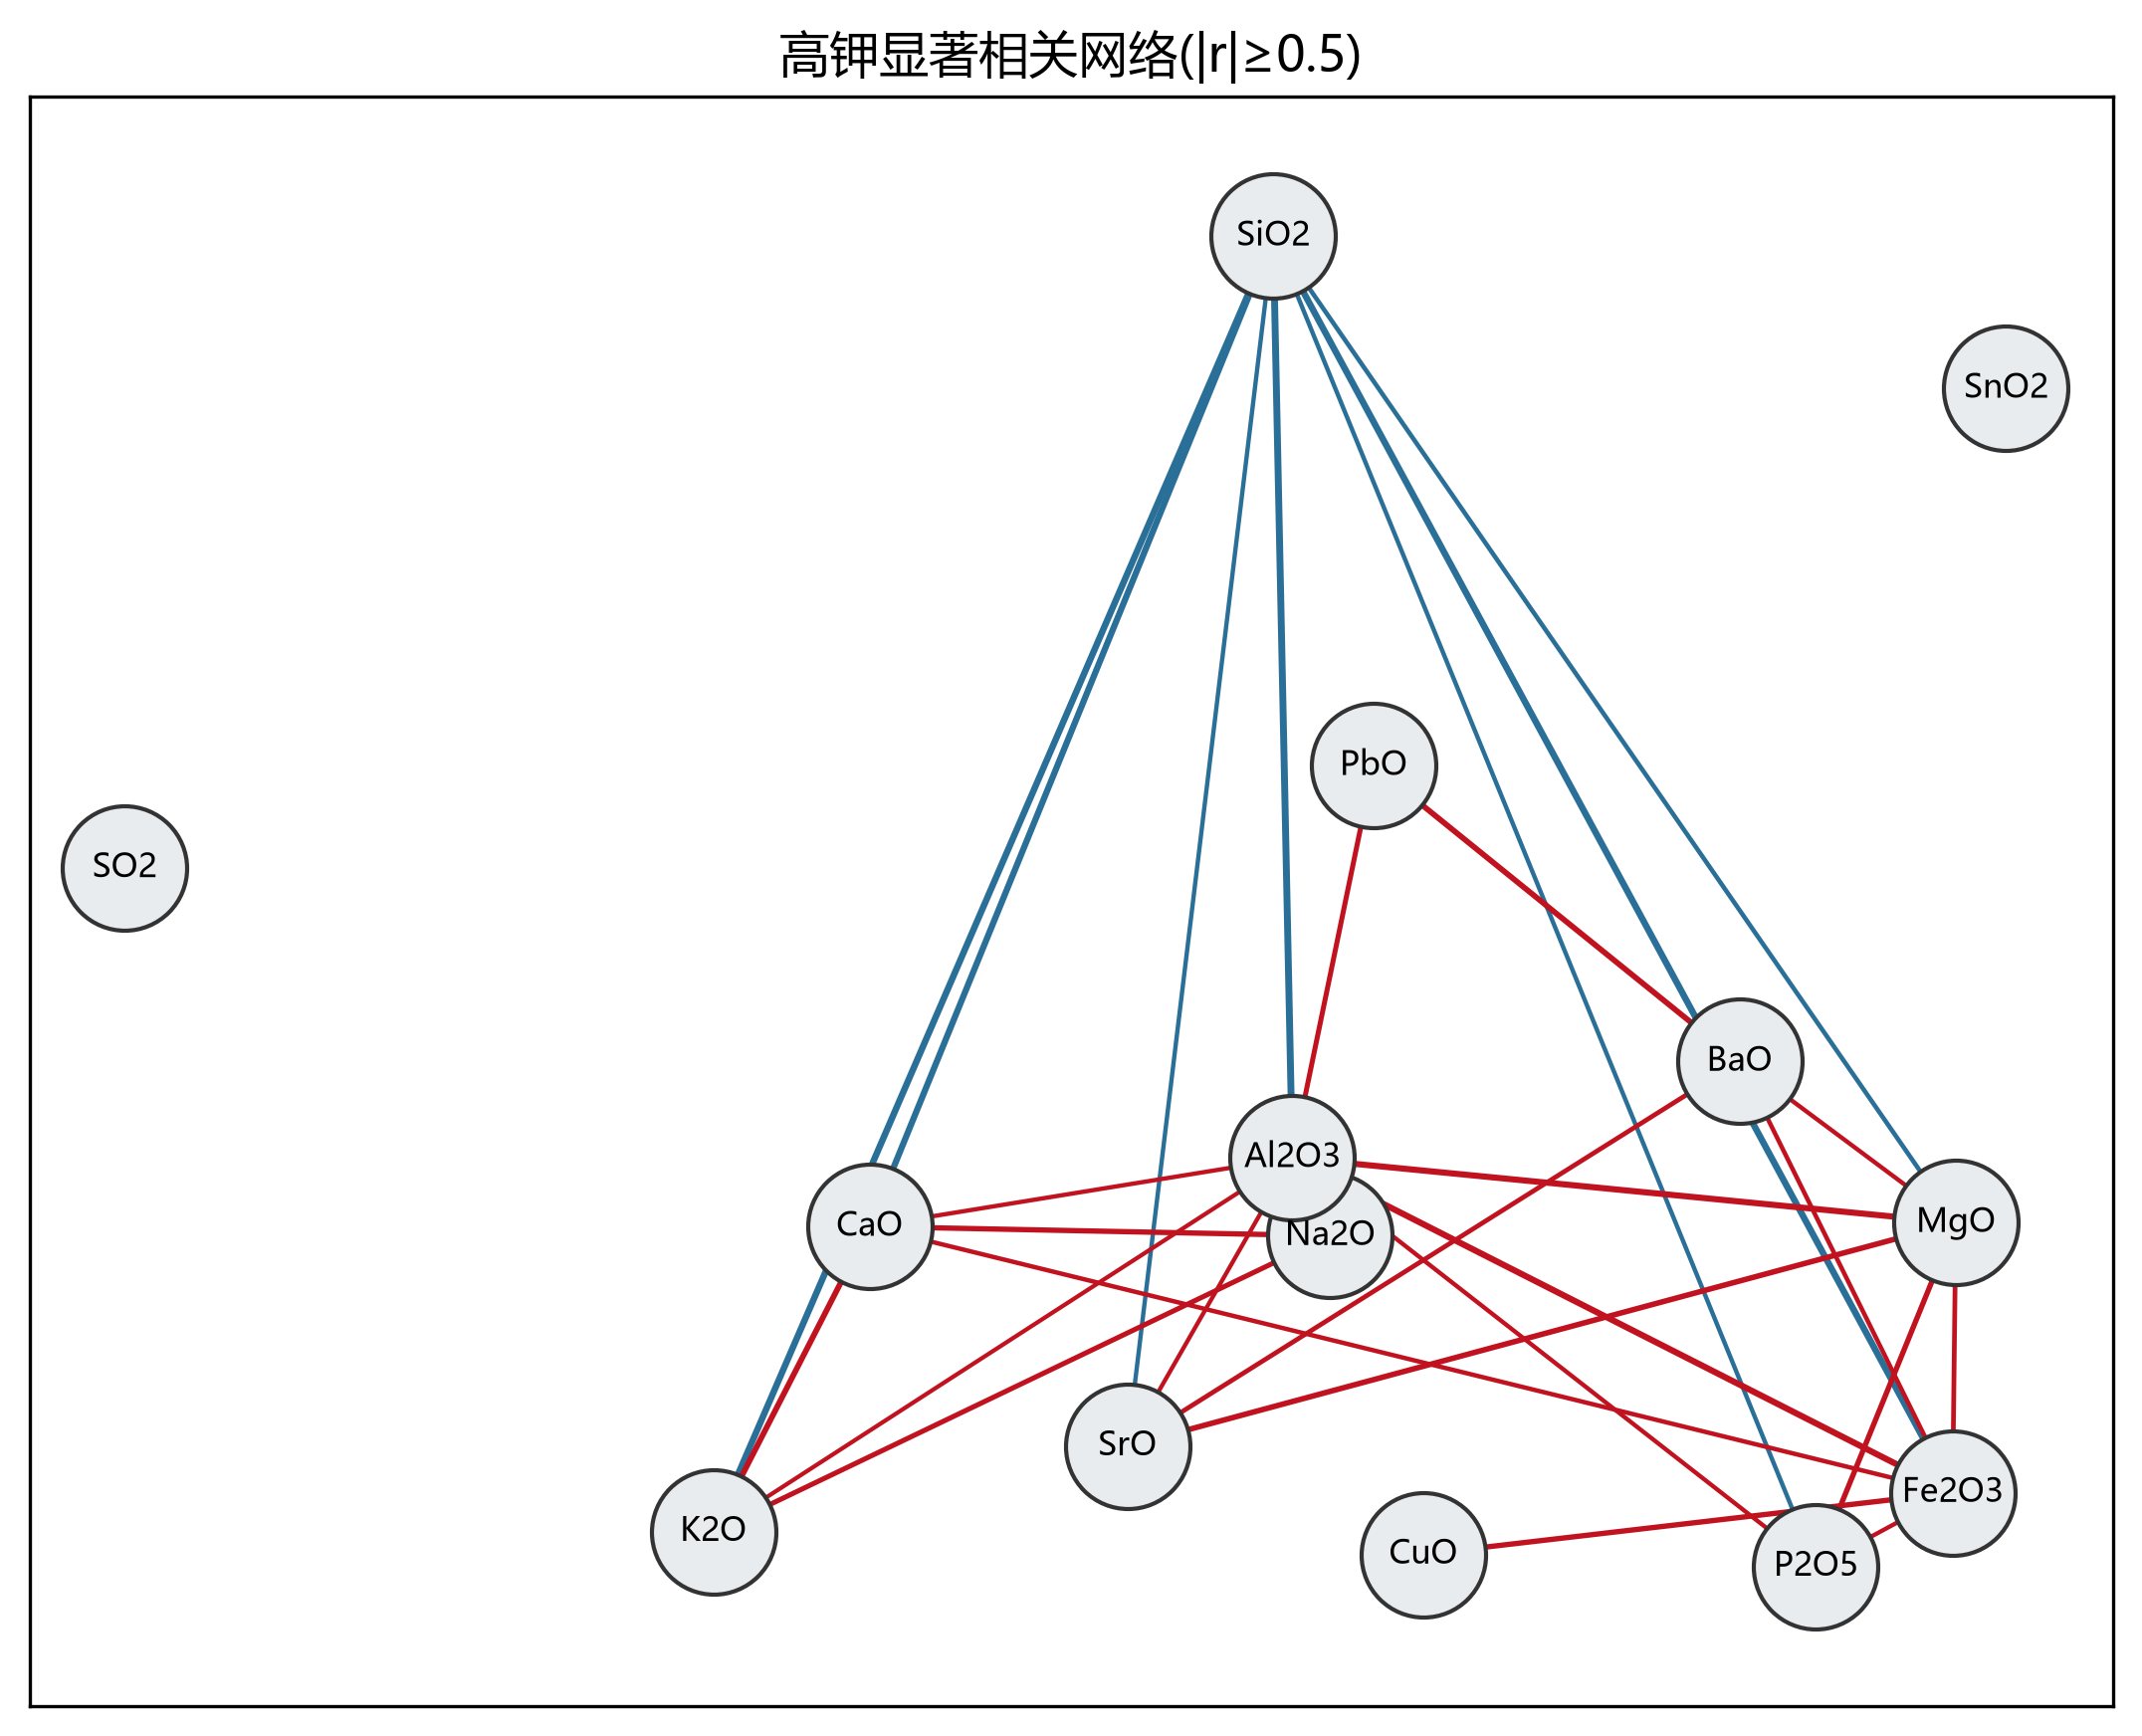
\includegraphics[width=\linewidth]{figures/q4_network_高钾.png}
\caption{高钾显著相关网络}
\label{fig:nethk}
\end{minipage}
\hfill
\begin{minipage}{0.48\textwidth}
\centering
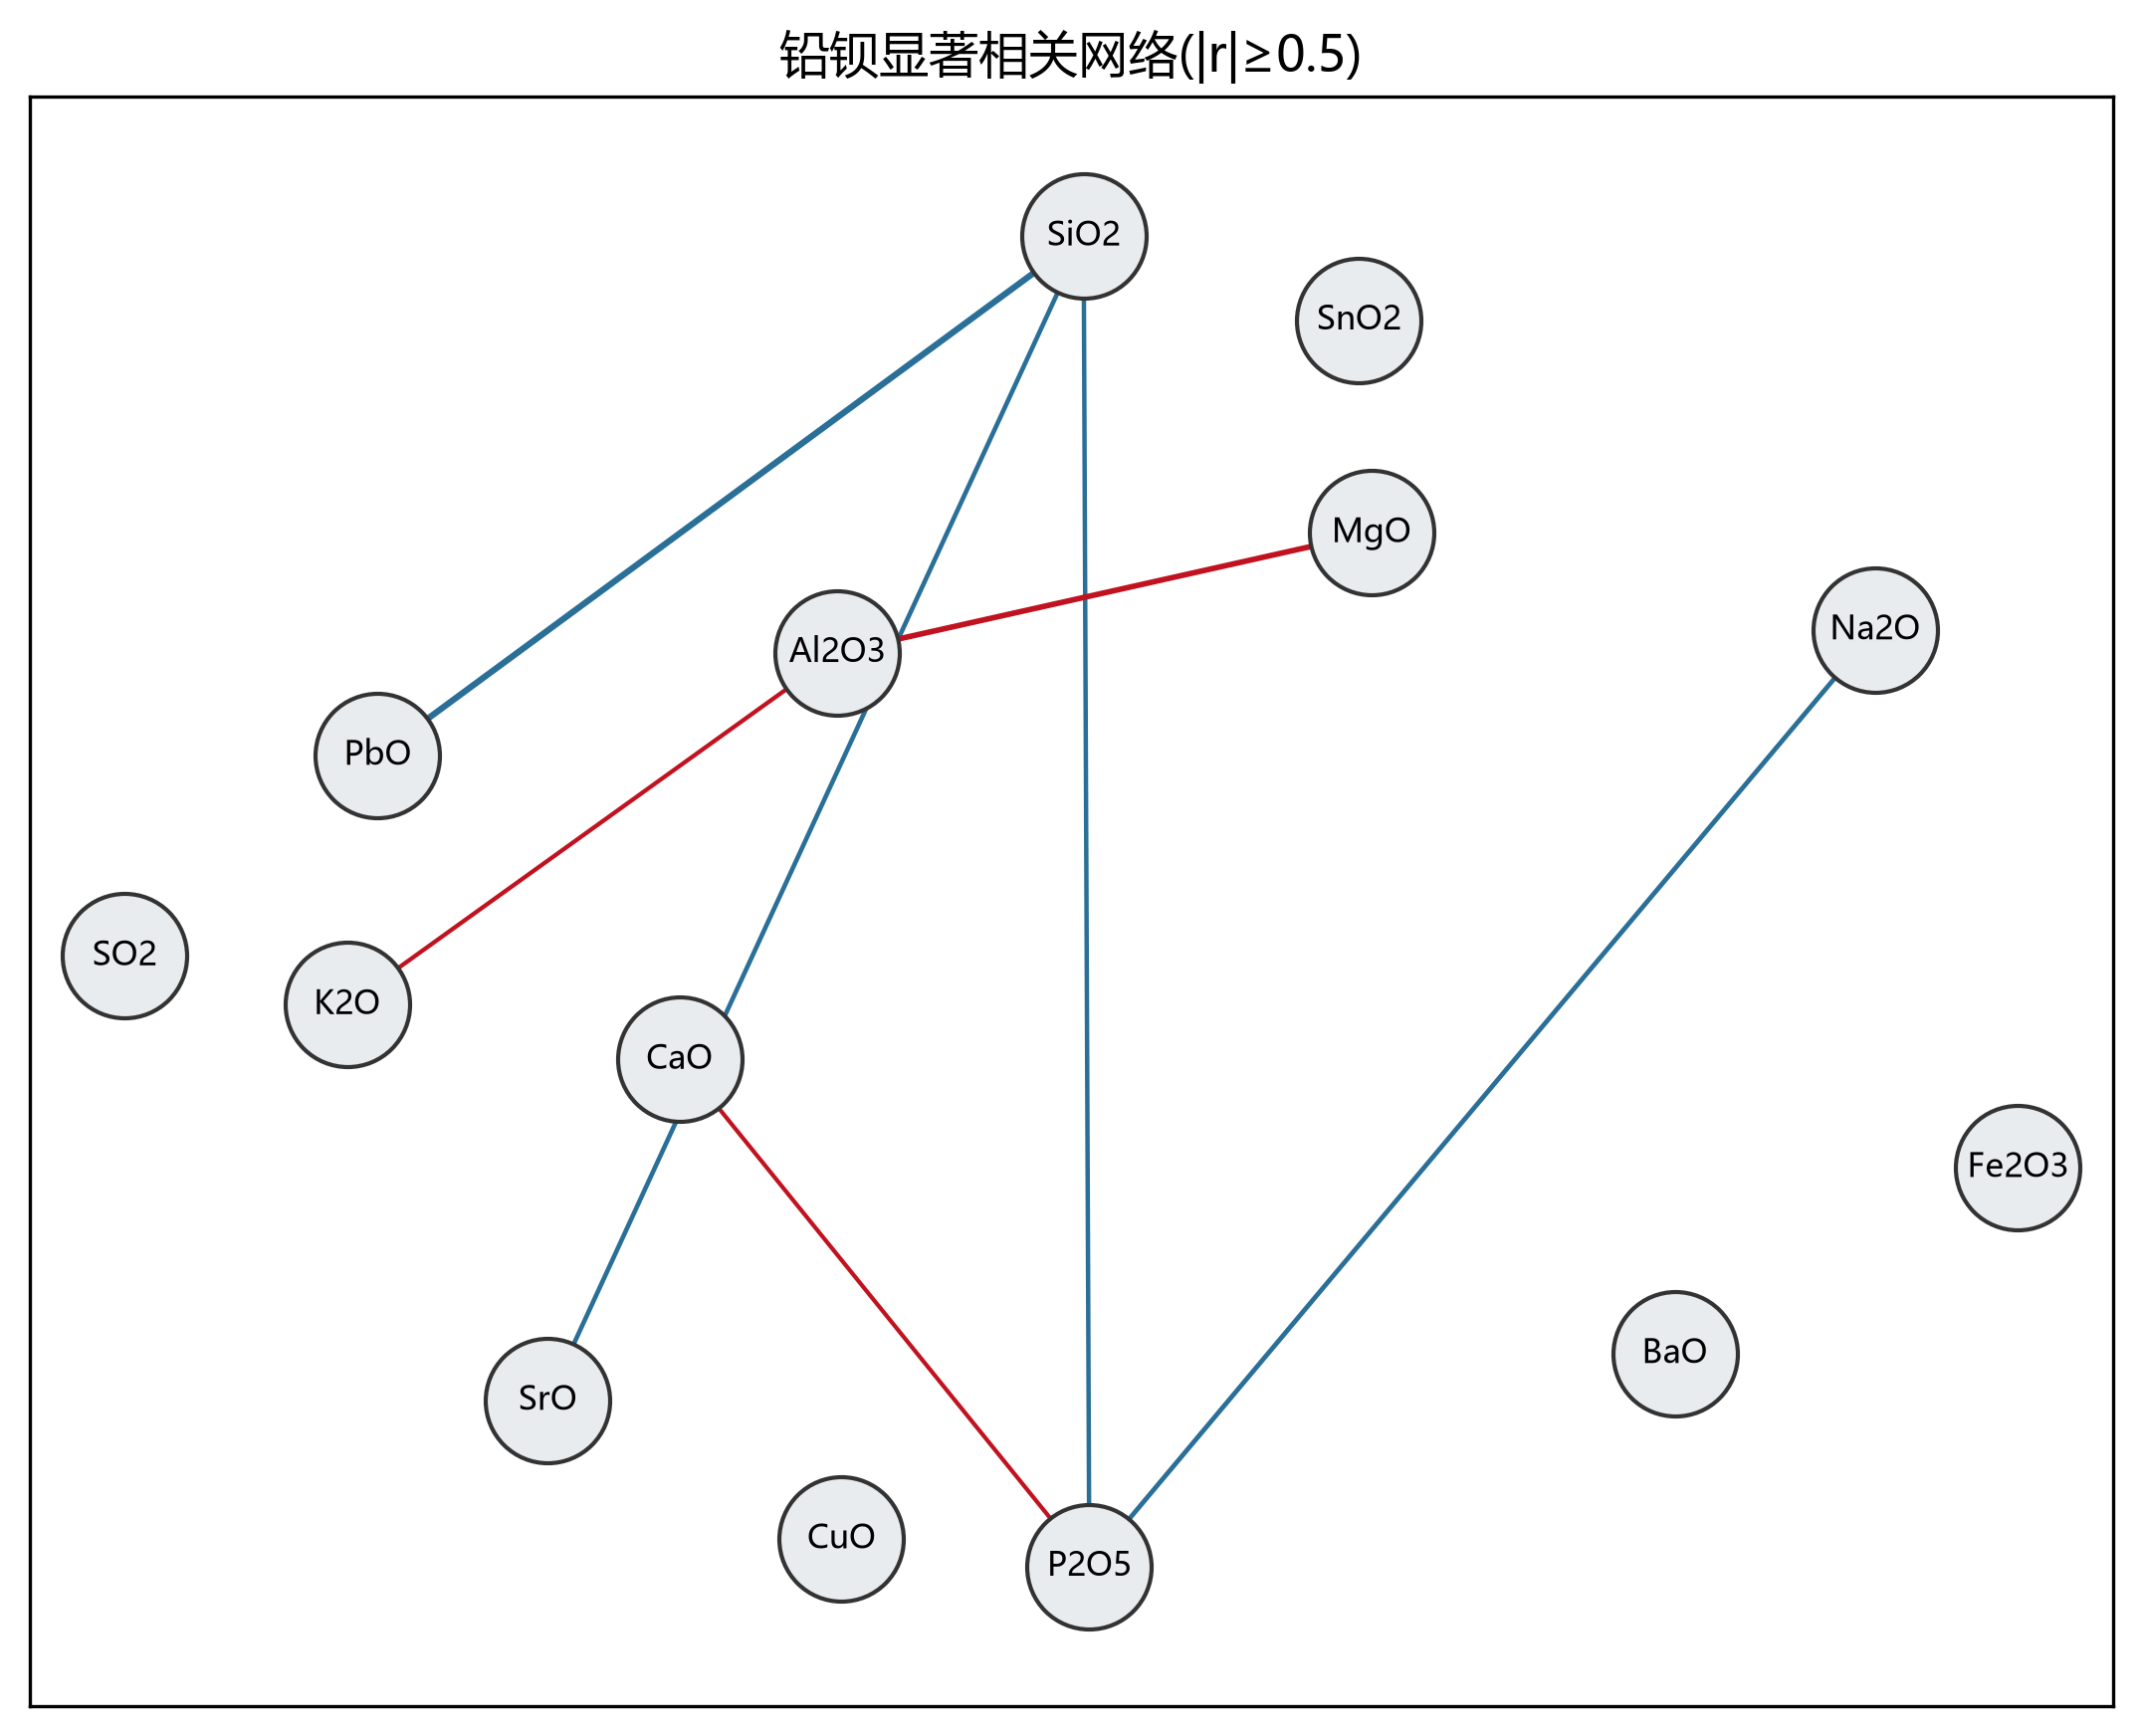
\includegraphics[width=\linewidth]{figures/q4_network_铅钡.png}
\caption{铅钡显著相关网络}
\label{fig:netpb}
\end{minipage}
\end{figure}

\subsection{差异性比较}
定义相关差矩阵$\Delta=R^{(\text{高钾})}-R^{(\text{铅钡})}$（公共成分），并用Mantel检验评估两相关矩阵相似性。得到$r=$0.1276，$p=$0.2050；平均$|\Delta r|=$0.377。最大差异成分对排序见表~\ref{tab:diff}与图~\ref{fig:diff}--\ref{fig:dheat}。

\begin{table}[H]
\centering
\caption{相关结构差异最大的成分对（Top）}
\label{tab:diff}
\scriptsize
\begin{tabular}{lcccc}
\toprule
成分A & 成分B & 高钾r & 铅钡r & 绝对差值 \\
\hline
Al2O3 & SiO2 & -0.831 & 0.425 & 1.255 \\
K2O & SiO2 & -0.781 & 0.308 & 1.089 \\
CuO & Fe2O3 & 0.643 & -0.390 & 1.032 \\
CaO & Na2O & 0.640 & -0.367 & 1.007 \\
Al2O3 & PbO & 0.602 & -0.389 & 0.991 \\
BaO & Fe2O3 & 0.539 & -0.443 & 0.981 \\
BaO & MgO & 0.521 & -0.435 & 0.956 \\
Na2O & SiO2 & -0.475 & 0.405 & 0.880 \\
Al2O3 & BaO & 0.473 & -0.369 & 0.842 \\
Fe2O3 & SiO2 & -0.783 & 0.044 & 0.826 \\
\bottomrule
\end{tabular}
\end{table}

\begin{figure}[H]
\centering
\begin{minipage}{0.48\textwidth}
\centering
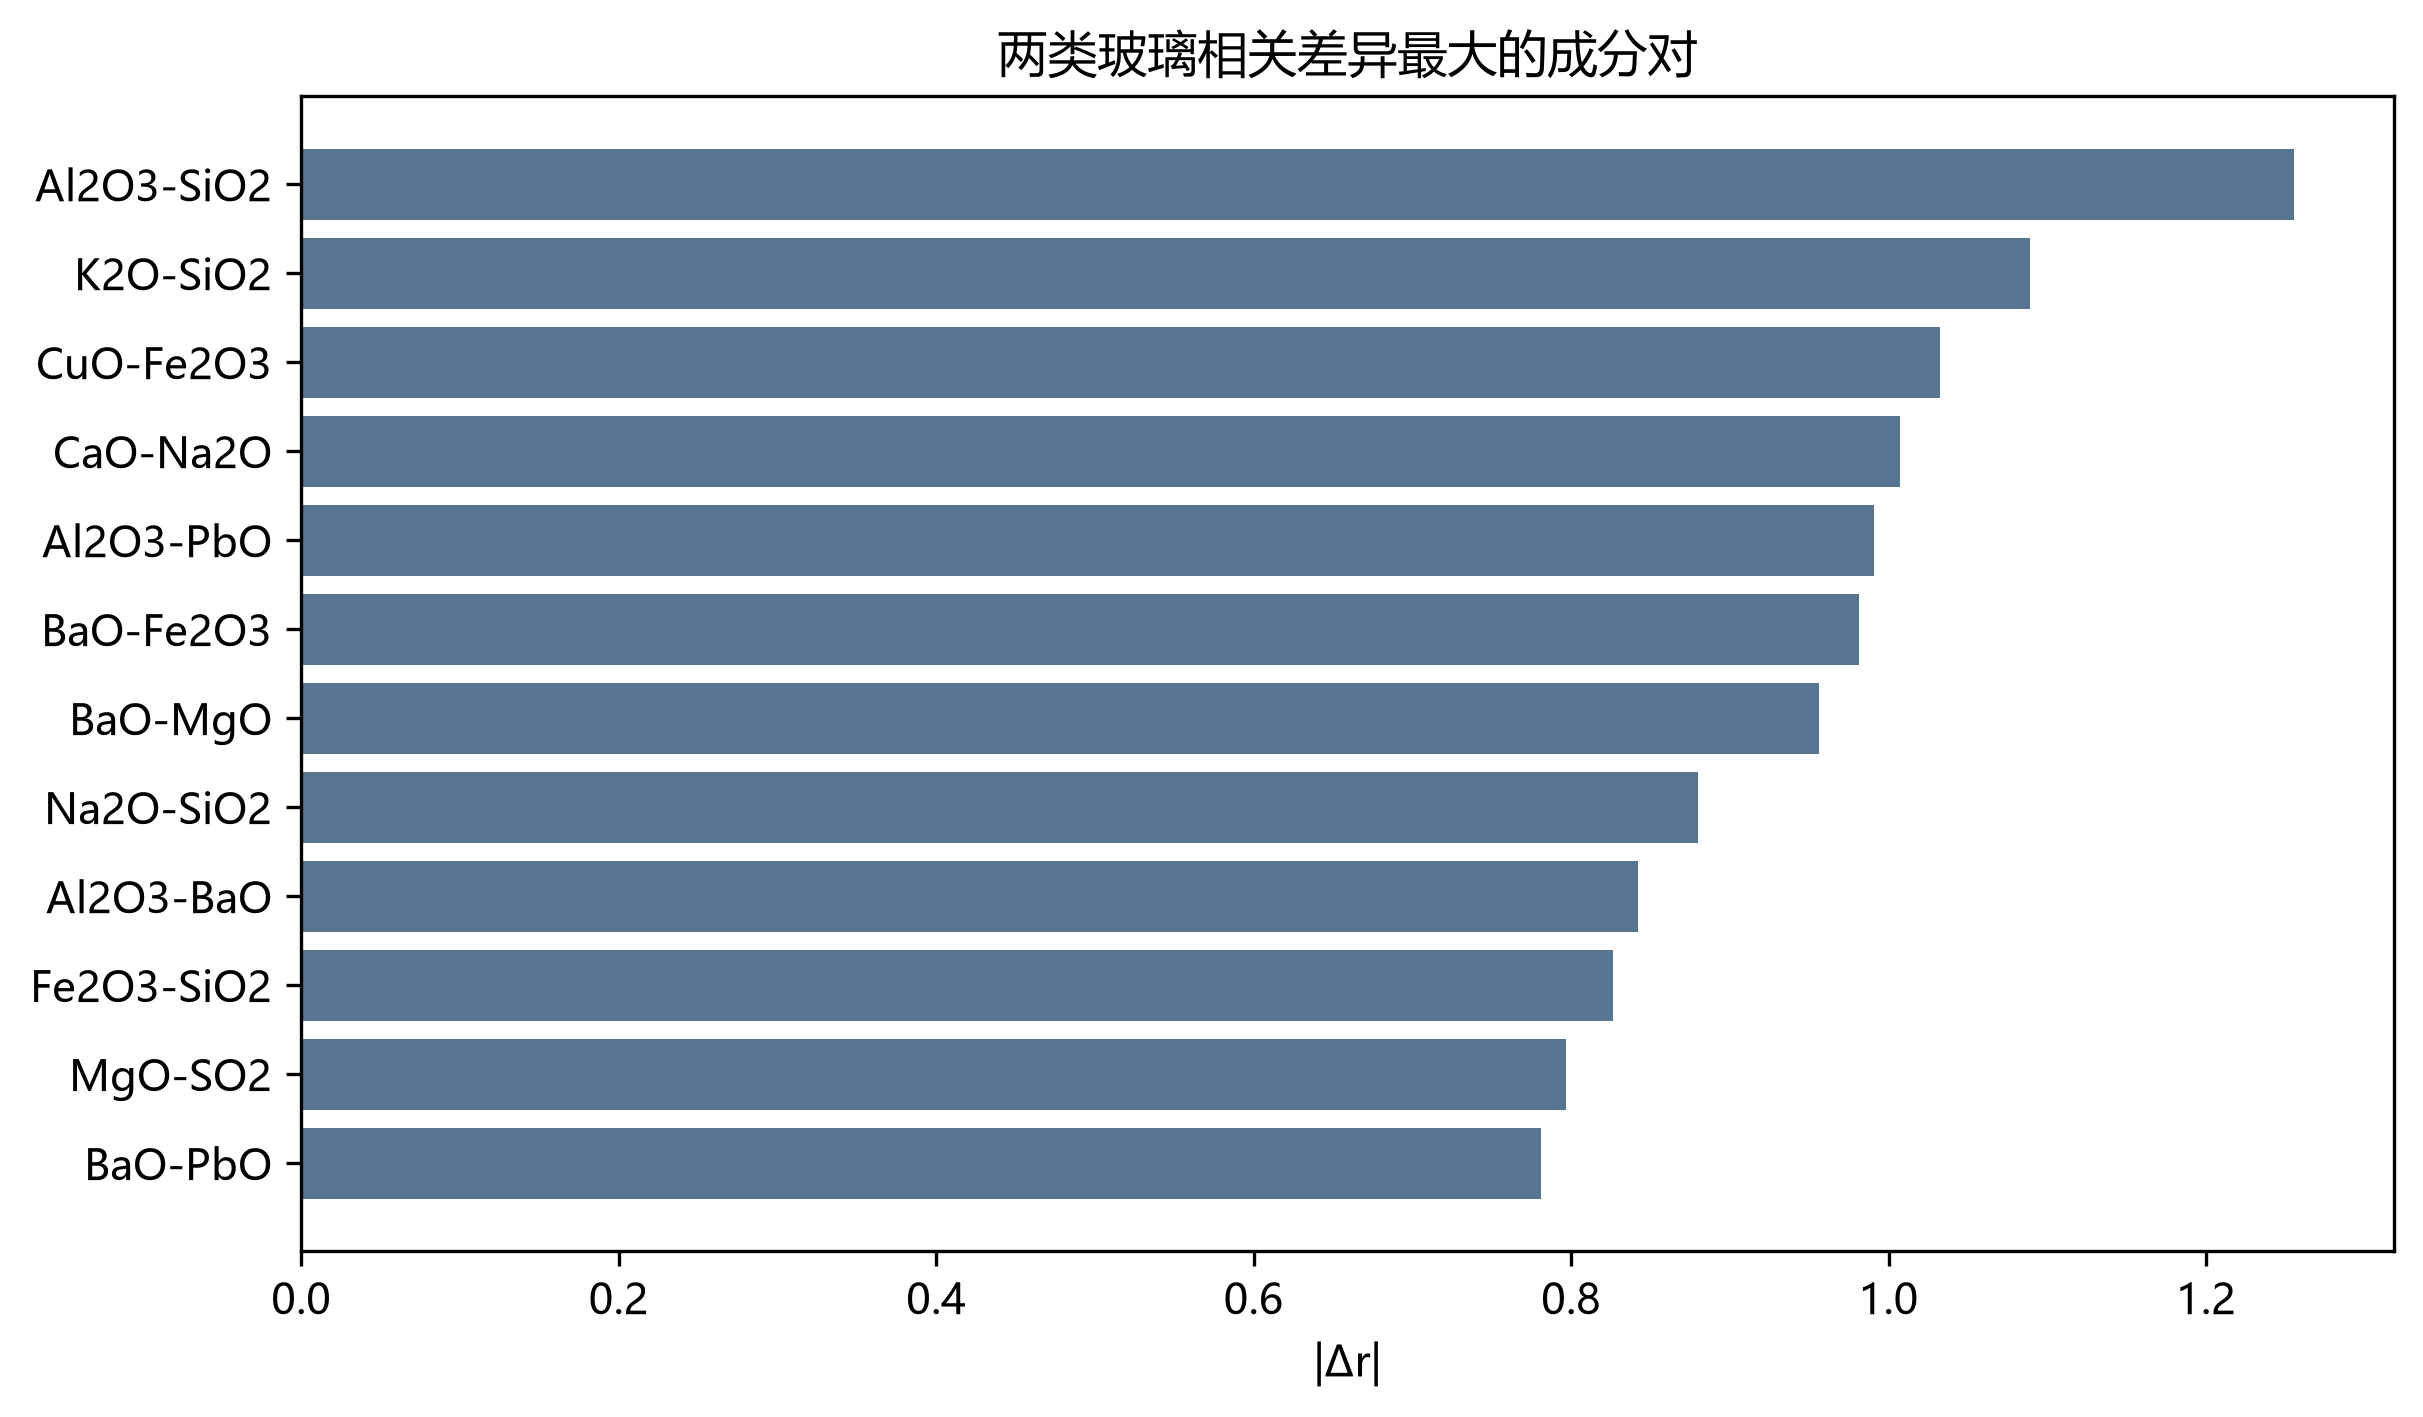
\includegraphics[width=\linewidth]{figures/q4_top_diff_pairs.png}
\caption{类别间$|\Delta r|$最大成分对}
\label{fig:diff}
\end{minipage}
\hfill
\begin{minipage}{0.48\textwidth}
\centering
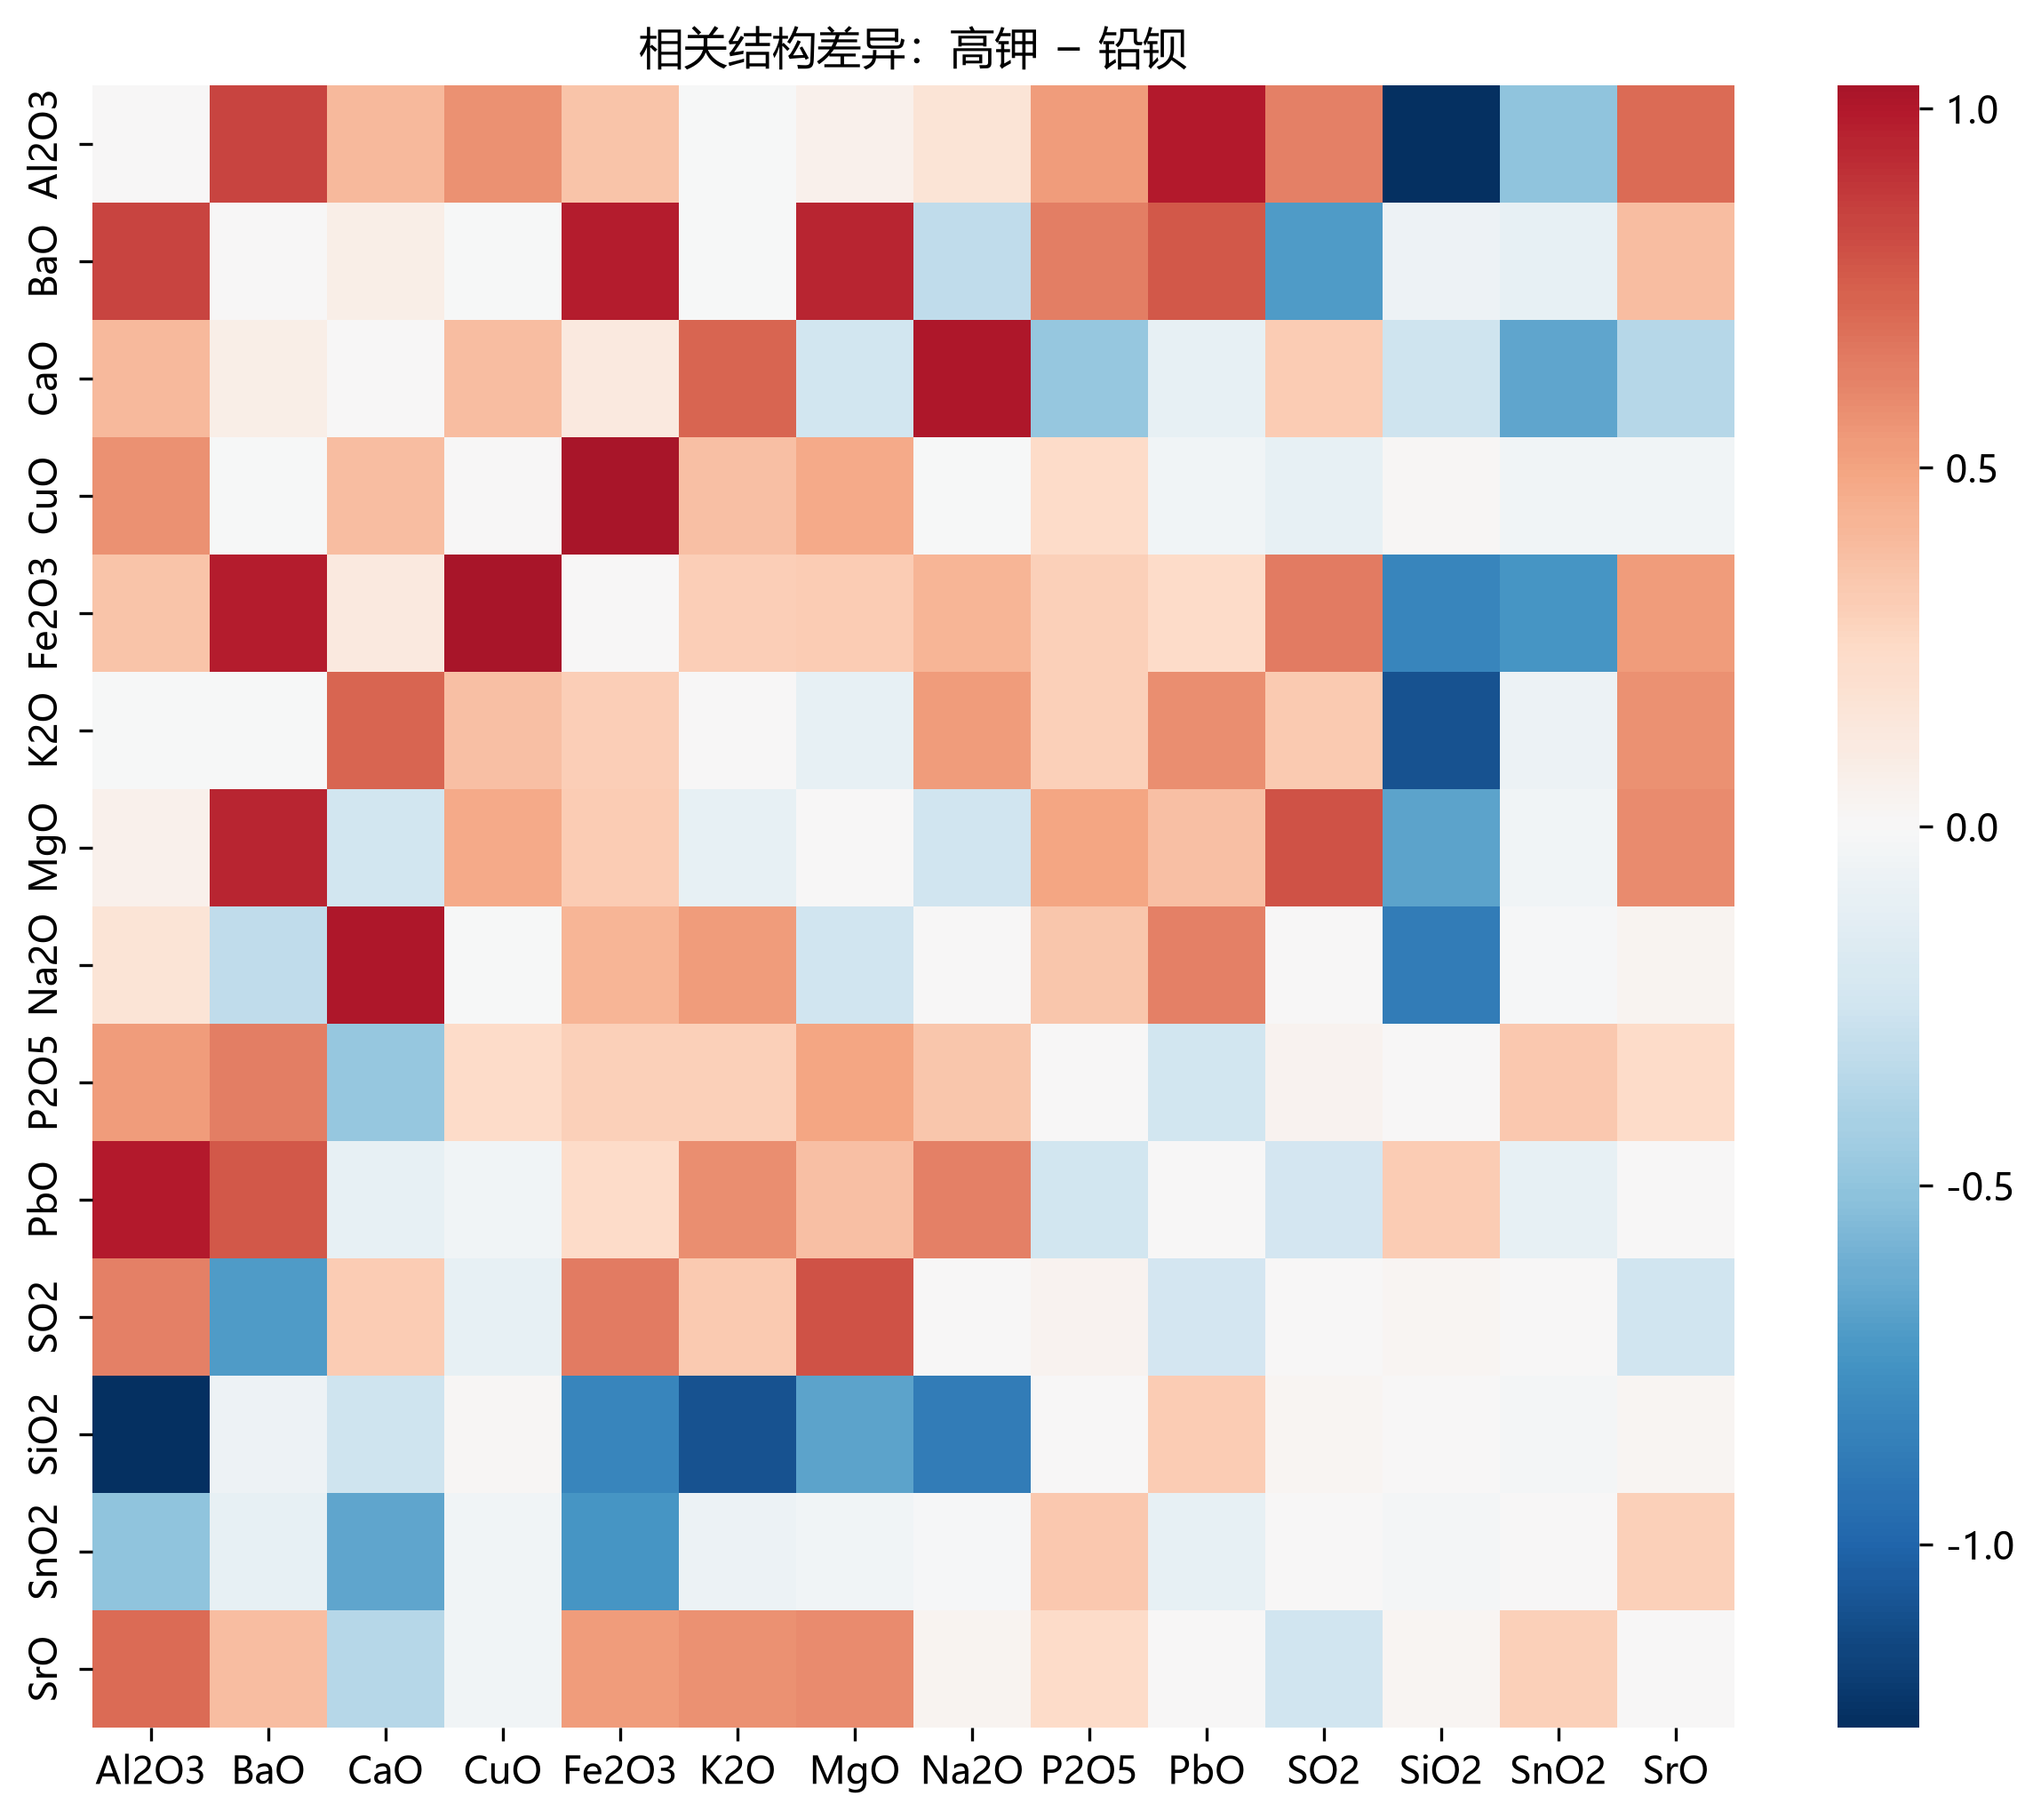
\includegraphics[width=\linewidth]{figures/q4_corr_diff_heatmap.png}
\caption{相关差热力图（高钾$-$铅钡）}
\label{fig:dheat}
\end{minipage}
\end{figure}

\section{模型检验}
\subsection{有效性对比与消融}
特征消融见表~\ref{tab:ab}与图~\ref{fig:ab}：仅用PbO+BaO已有较强可分性，但扩展到核心四成分/全部主特征可进一步提升或稳定F1，说明多氧化物信息对边界样本有价值。

\begin{table}[H]
\centering
\caption{特征消融结果}
\label{tab:ab}
\scriptsize
\begin{tabular}{lccc}
\toprule
特征集 & LOO准确率 & MacroF1 & 特征数 \\
\hline
仅SiO2+K2O & 0.970 & 0.962 & 2 \\
仅PbO+BaO & 1.000 & 1.000 & 2 \\
核心四成分 & 1.000 & 1.000 & 4 \\
全部主特征 & 1.000 & 1.000 & 10 \\
\bottomrule
\end{tabular}
\end{table}

\begin{figure}[H]
\centering
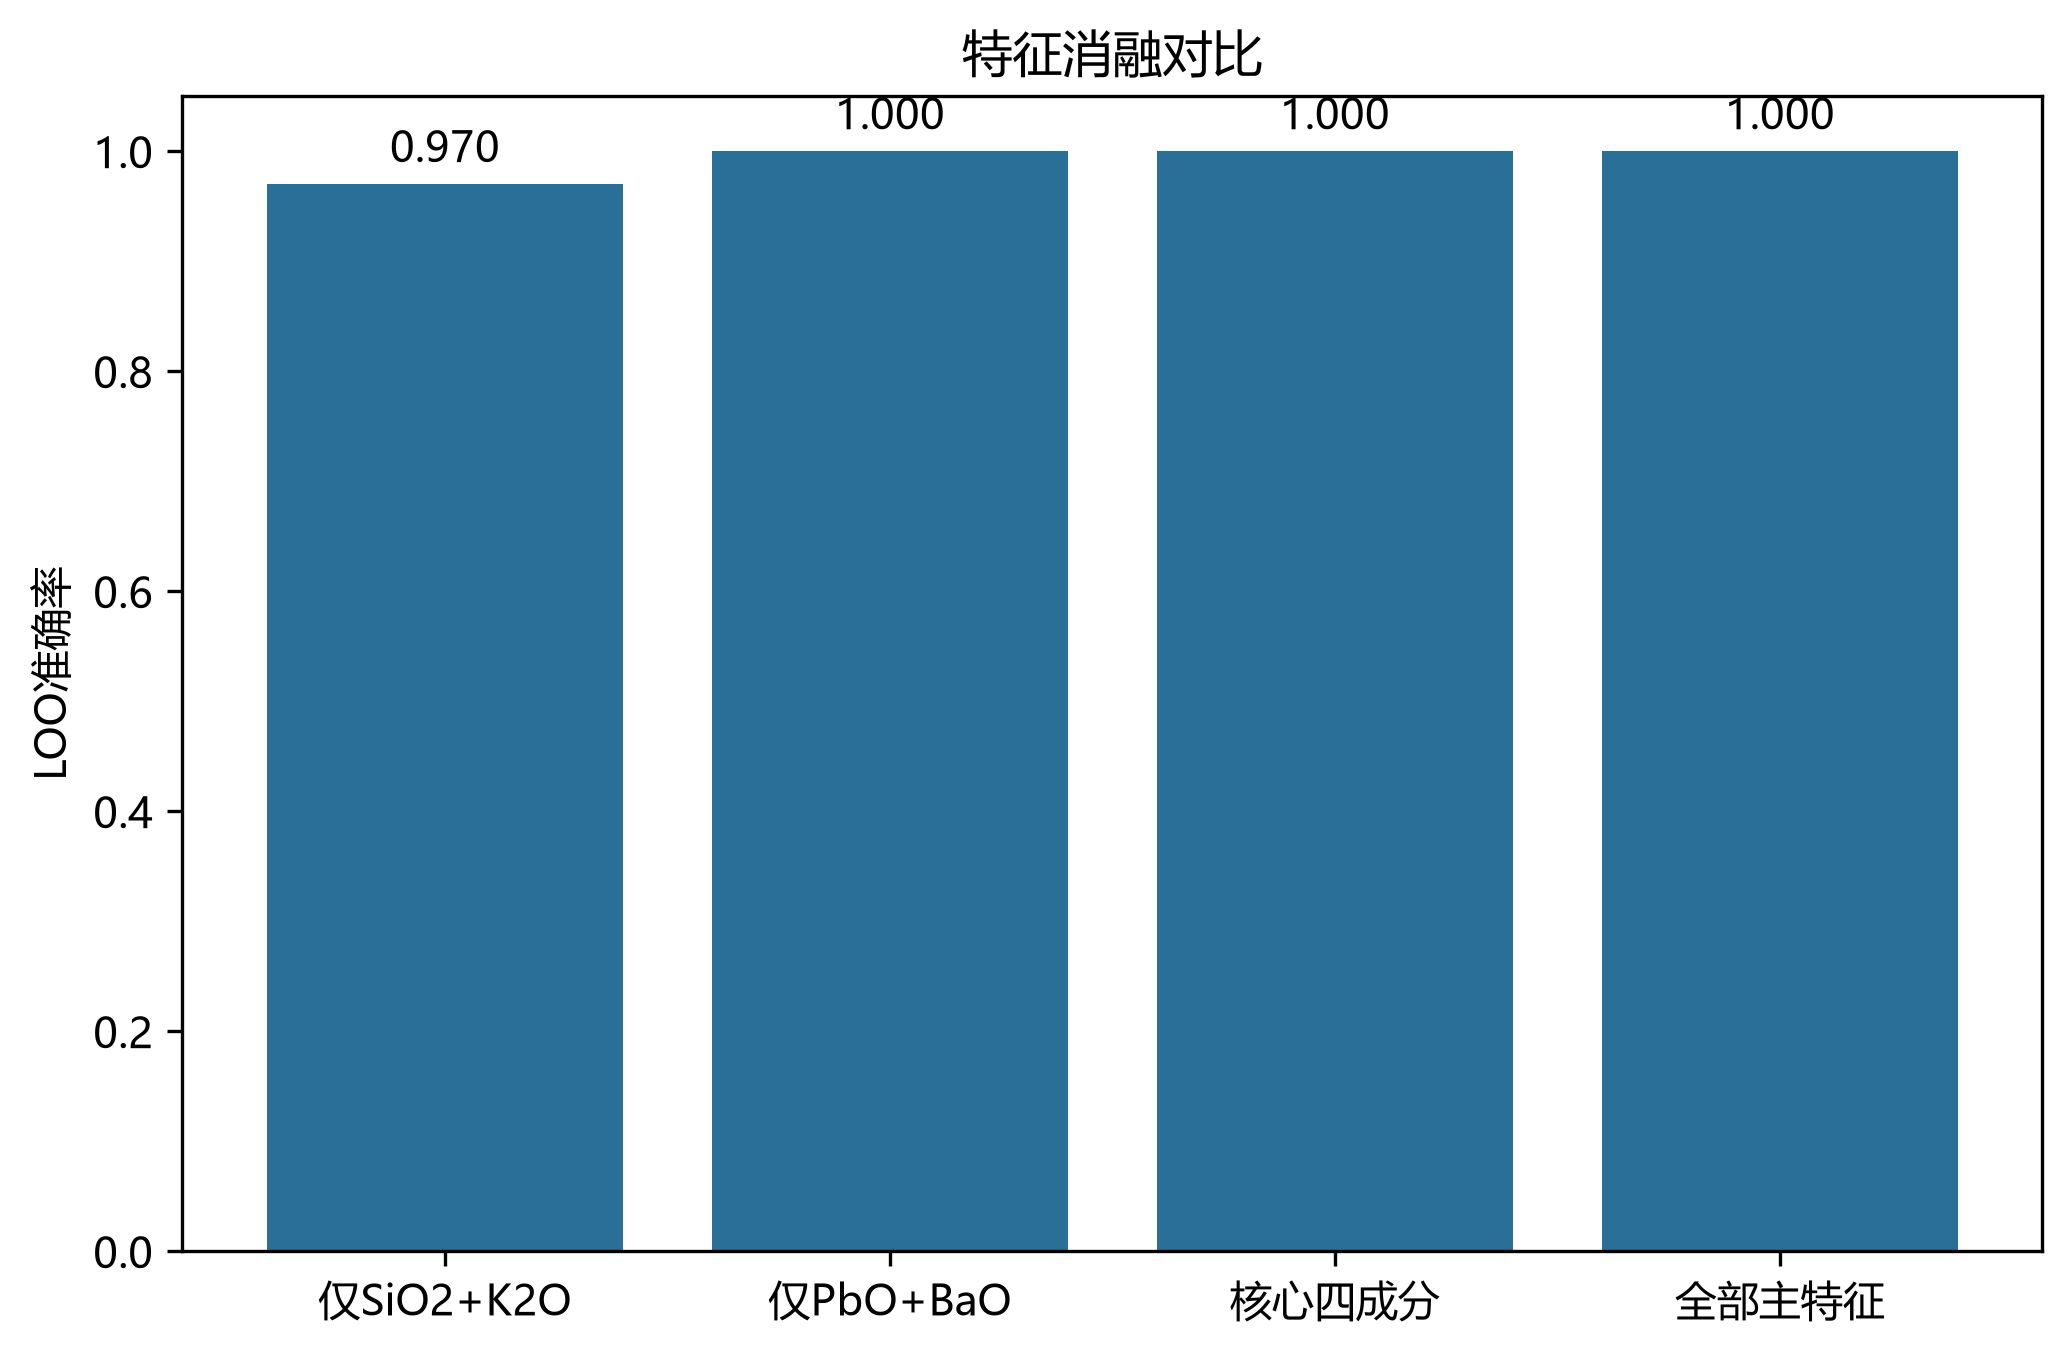
\includegraphics[width=0.75\textwidth]{figures/adv_ablation_features.png}
\caption{特征消融对比}
\label{fig:ab}
\end{figure}

风化分层准确率见表~\ref{tab:strat}与图~\ref{fig:strat}，用于检查模型是否被风化状态系统性误导。

\begin{table}[H]
\centering
\caption{风化分层分类准确率}
\label{tab:strat}
\scriptsize
\begin{tabular}{lcc}
\toprule
子集 & n & 准确率 \\
\hline
全体 & 67 & 1.000 \\
风化 & 32 & 1.000 \\
无风化 & 35 & 1.000 \\
\bottomrule
\end{tabular}
\end{table}

\begin{figure}[H]
\centering
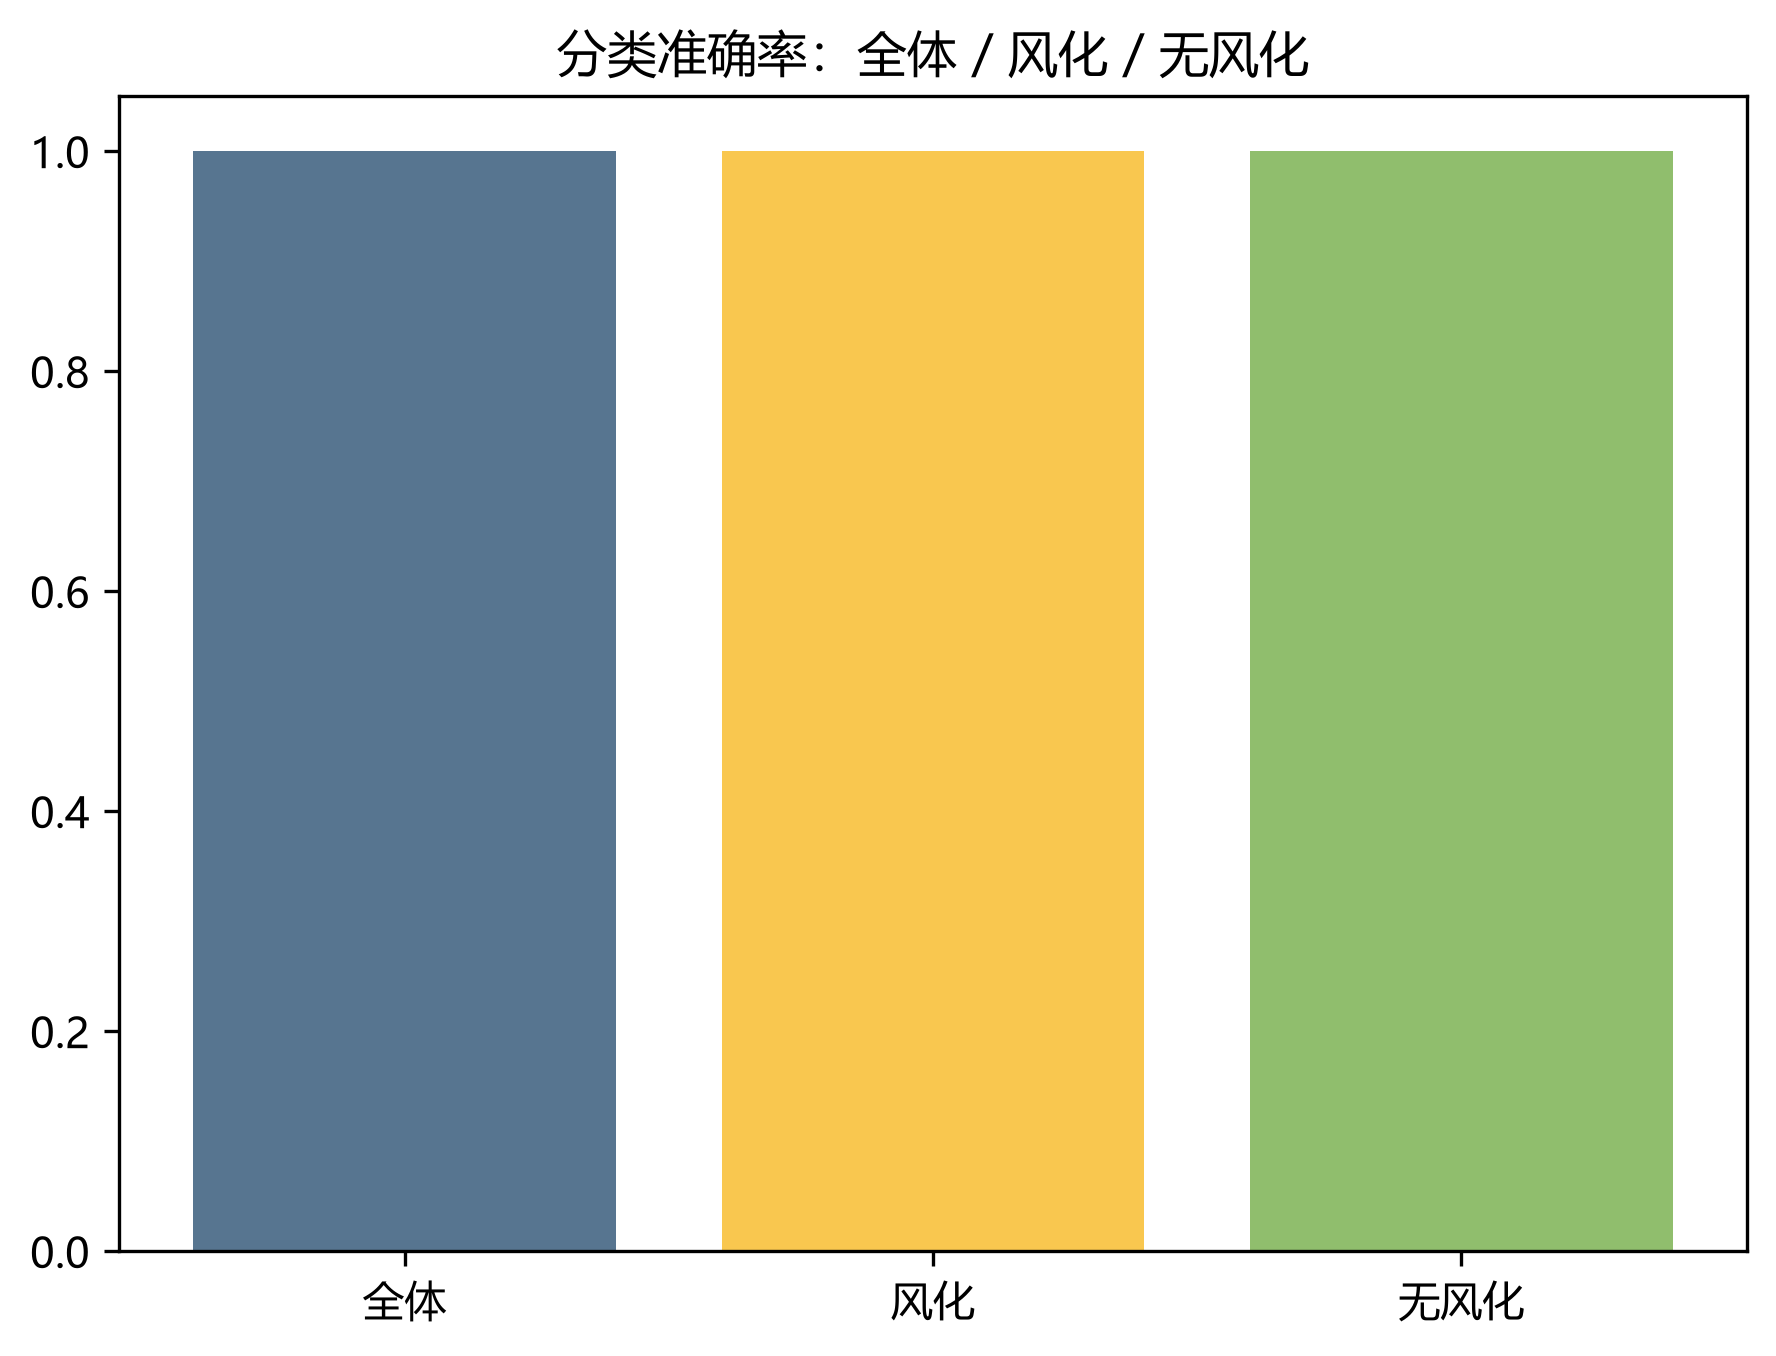
\includegraphics[width=0.7\textwidth]{figures/adv_weather_stratified_acc.png}
\caption{全体/风化/无风化准确率}
\label{fig:strat}
\end{figure}

\subsection{鲁棒性（蒙特卡洛）}
对训练成分施加相对噪声并反复预测，准确率分布见图~\ref{fig:mc}：均值1.0000，5\%--95\%分位$[1.0000,1.0000]$，不低于$0.9$的概率100.00\%。

\begin{figure}[H]
\centering
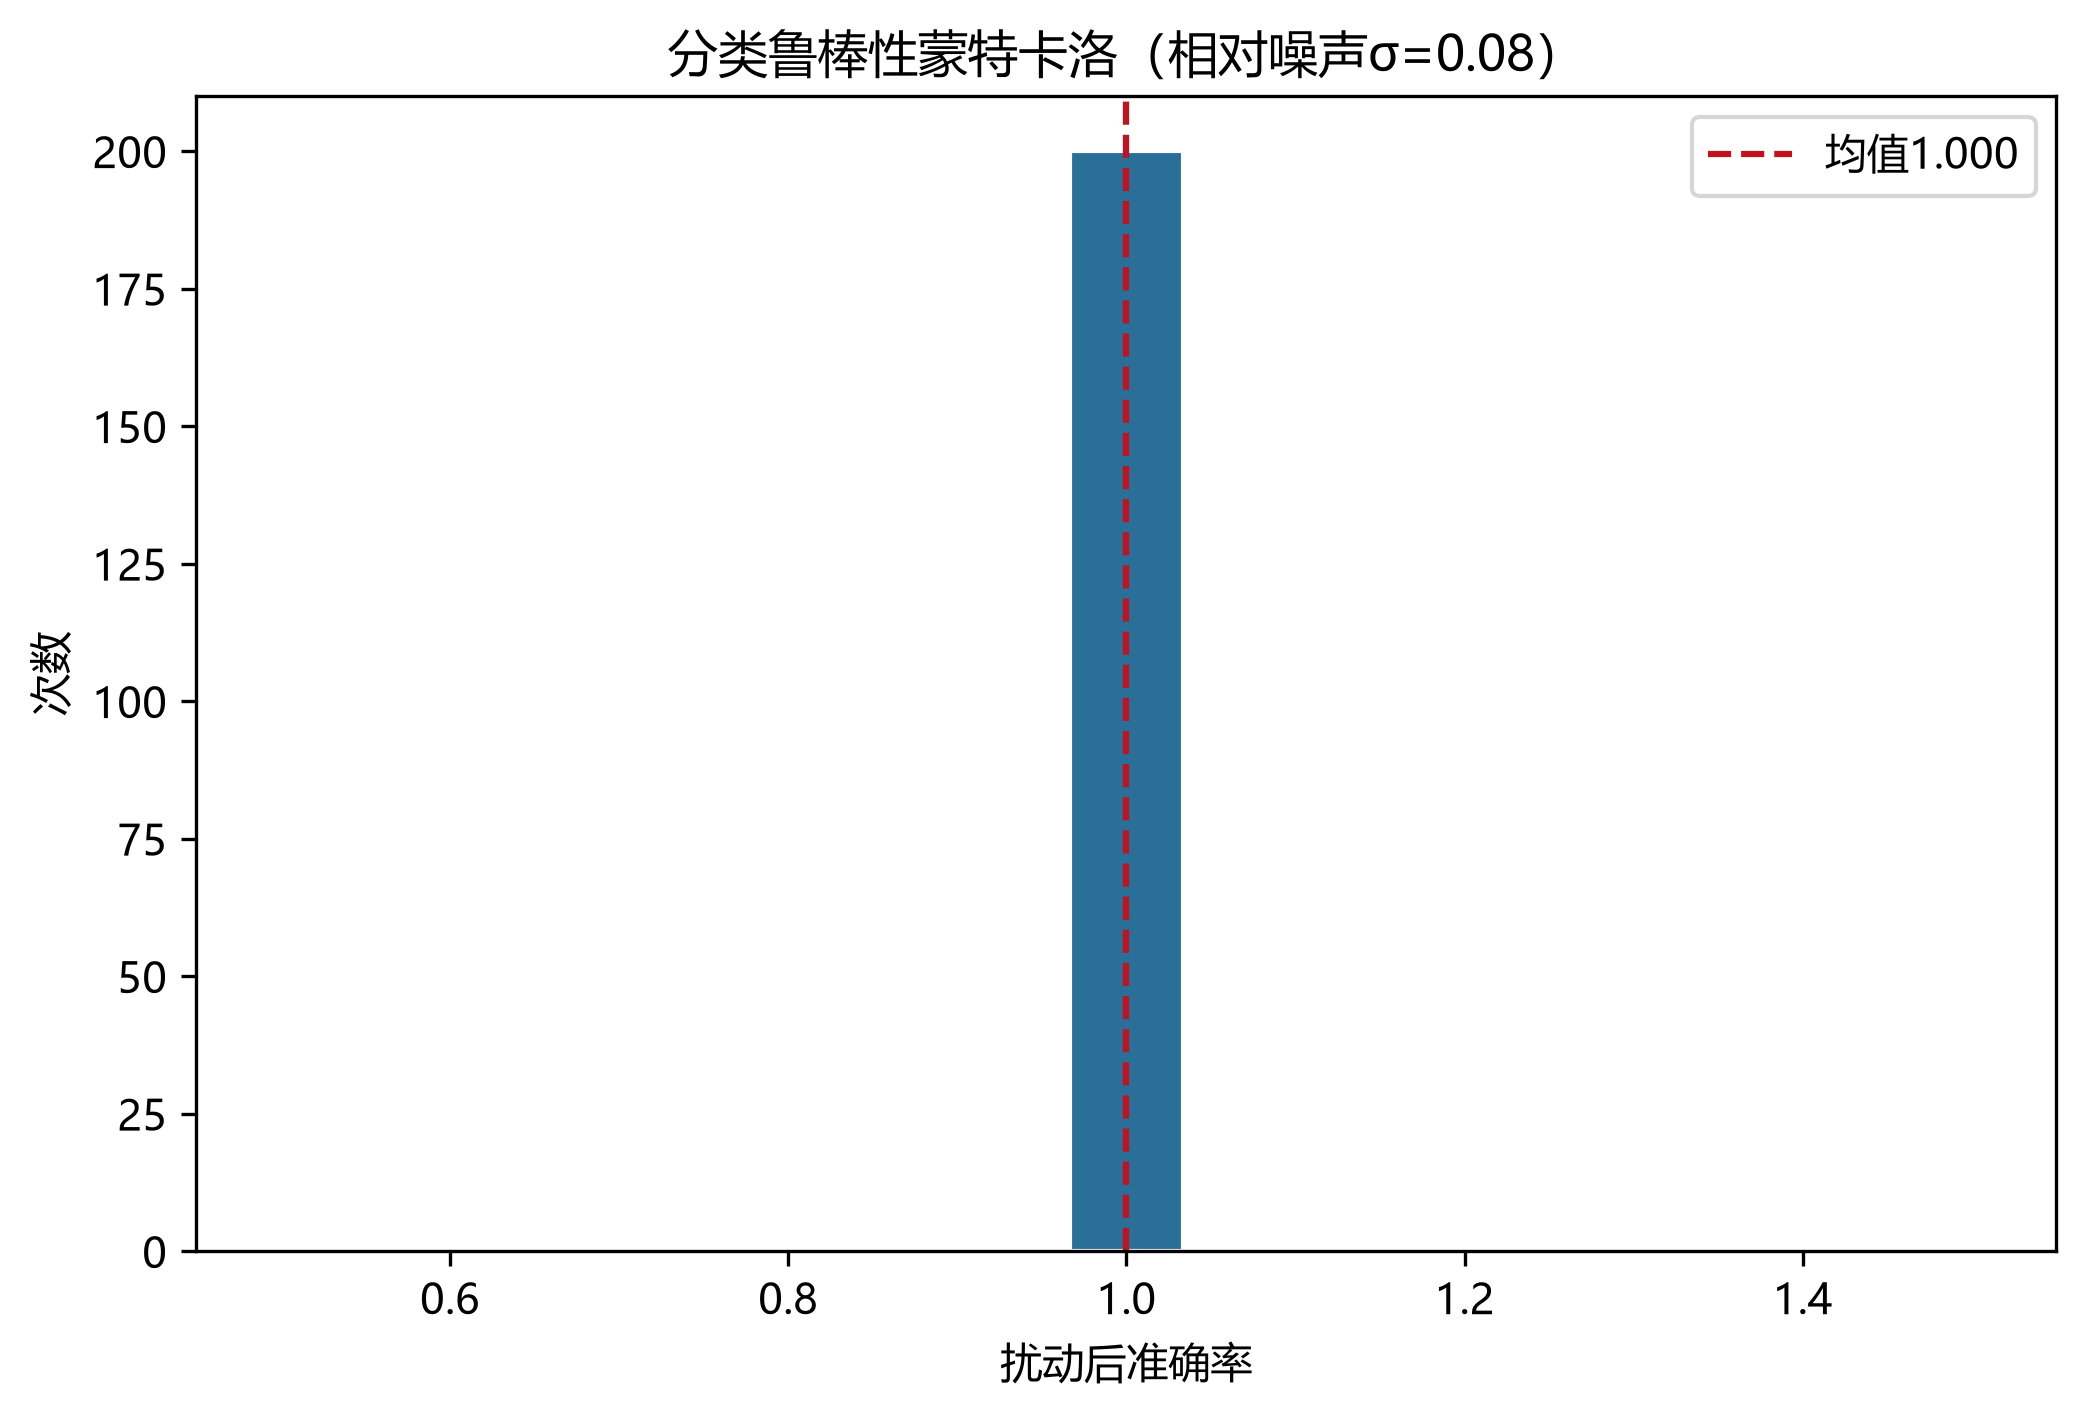
\includegraphics[width=0.75\textwidth]{figures/adv_mc_acc_hist.png}
\caption{分类准确率蒙特卡洛分布}
\label{fig:mc}
\end{figure}

\subsection{误差与局限}
\begin{enumerate}[leftmargin=2em]
\item 风化因子基于组间均值，难以刻画同一文物不同部位的非线性风化；
\item 空白按0填充会压缩极低含量成分的变异；
\item 未知样本若处于两类重叠区，置信度与翻转率应同时解读；
\item 亚类数由轮廓系数选择，解释需结合考古工艺知识，不宜过度本体论化。
\end{enumerate}

\section{模型评价与推广}
\subsection{优点}
形成了从风化机制到类型鉴别再到关联结构的统一框架；强调可解释规则与统计学习对照；检验覆盖灵敏度与鲁棒性。

\subsection{创新点}
\begin{enumerate}[leftmargin=2em]
\item 类型条件风化因子反演及与无校正/差值校正的定量对比；
\item 规则--学习双轨分类 + 特征消融，明确Pb/Ba主导与多特征增益；
\item 未知样本的概率、噪声翻转与训练留一稳定性三重证据；
\item Mantel与$|\Delta r|$排序的相关结构差异性检验；
\item 风化分层准确率与整体MC鲁棒性闭环。
\end{enumerate}

\subsection{推广}
方法可推广至陶瓷胎釉成分甄别、金属器合金风化校正与产地溯源等“成分性数据 + 环境蚀变”问题。

\section{参考文献}
\begin{thebibliography}{99}
\bibitem{cumcm2022c} 全国大学生数学建模竞赛组委会. 2022年高教社杯全国大学生数学建模竞赛题目C题[Z]. 2022.
\bibitem{breiman2001} Breiman L. Random forests[J]. Machine Learning, 2001, 45(1): 5-32.
\bibitem{cover1967} Cover T, Hart P. Nearest neighbor pattern classification[J]. IEEE Trans. Inf. Theory, 1967, 13(1): 21-27.
\bibitem{cortes1995} Cortes C, Vapnik V. Support-vector networks[J]. Machine Learning, 1995, 20(3): 273-297.
\bibitem{spearman1904} Spearman C. The proof and measurement of association between two things[J]. Am. J. Psychol., 1904, 15: 72-101.
\bibitem{mantel1967} Mantel N. The detection of disease clustering and a generalized regression approach[J]. Cancer Res., 1967, 27(2): 209-220.
\bibitem{rousseeuw1987} Rousseeuw P J. Silhouettes: a graphical aid to the interpretation and validation of cluster analysis[J]. J. Comput. Appl. Math., 1987, 20: 53-65.
\bibitem{aitchison1986} Aitchison J. The Statistical Analysis of Compositional Data[M]. Chapman and Hall, 1986.
\bibitem{fisher1922} Fisher R A. On the interpretation of $\chi^2$ from contingency tables[J]. J. R. Stat. Soc., 1922, 85(1): 87-94.
\bibitem{mann1947} Mann H B, Whitney D R. On a test of whether one of two random variables is stochastically larger than the other[J]. Ann. Math. Stat., 1947, 18(1): 50-60.
\end{thebibliography}

\appendix
\section{附录：决策树规则文本}
决策树（深度3）导出的分割规则保存于配套文件\texttt{output/tables/q2\_decision\_tree\_rules.txt}，可用于考古场景的快速人工复核。

\section{附录：核心代码说明}
一键复现入口为\texttt{python run\_all.py}，依次执行：预处理与EDA、Q1风化分析、Q2分类与亚类、Q3未知鉴别、Q4关联差异、高级检验、论文编译。代码位于\texttt{code/}目录，以脚本方式通过\texttt{sys.path}导入工具模块，避免将项目包装为遮蔽标准库的\texttt{code}包。

\section{附录：补充说明}
\begin{enumerate}[leftmargin=2em]
\item 统计口径：含量为质量百分比；有效样本成分和$\in[85\%,105\%]$；风化预测输出已归一化。
\item 论文图表由运行脚本自动生成并嵌入，数值与\texttt{output/results\_summary.md}及CSV一致。
\item 若需查看亚类中心坐标，参见\texttt{q2\_subclass\_centers\_*.csv}。
\end{enumerate}

\section{附录：实施效果与使用建议}
在考古实验室场景中，可按如下流程落地：
\begin{enumerate}[leftmargin=2em]
\item 录入或导入XRF/SEM-EDS成分表，自动计算成分和并过滤无效行；
\item 若样本标注为风化，先按类型调用风化因子反演，得到风化前估计谱；
\item 用随机森林给出类型概率，同时输出化学规则标签作交叉核对；
\item 当置信度低于$0.8$或噪声翻转率高于$0.2$时，建议补测未风化点或增加检测点位；
\item 对已分类样本，定期更新Spearman网络，监控配方结构是否出现新亚型。
\end{enumerate}

设判别器输出概率$\hat p_i$，定义风险分数
\begin{equation}
\mathrm{Risk}_i=(1-\mathrm{Conf}_i)+ \lambda \cdot \mathrm{Flip}_i,
\end{equation}
其中$\lambda>0$平衡置信度与扰动敏感性。该风险分数可用于实验排期：优先复测高风险样本，从而在有限检测预算下提升整体鉴别可靠度。

对亚类结果，建议与纹饰、颜色及出土地点做交叉表验证。若某一亚类在地理或纹饰上高度富集，则可解释为工艺传统差异；若完全随机，则提示聚类可能主要捕捉连续风化梯度，需要回到Q1校正后再划分。

\section{附录：更多公式推导}
\subsection{风化因子的一阶误差传播}
若观测存在相对误差$\delta$，即$x_{ic}'=x_{ic}(1+\delta)$，则反演
\begin{equation}
\hat x_{ic}^{(0)\prime}
=100\cdot\frac{x_{ic}'/f_{t,c}}{\sum_{c'}x_{ic}'/f_{t,c'}}
=100\cdot\frac{x_{ic}/f_{t,c}}{\sum_{c'}x_{ic}/f_{t,c'}}
=\hat x_{ic}^{(0)}.
\end{equation}
说明：在全部成分同比例缩放时，归一化反演对全局倍率误差不敏感；真正影响结果的是\textbf{成分间相对比例}被风化扭曲的部分，这也是需要按类型估计$f_{t,c}$的原因。

\subsection{随机森林投票的置信度含义}
对$B$棵树，
\begin{equation}
\mathrm{Conf}_i=\max_y \frac{1}{B}\sum_{b=1}^{B}\mathbf{1}(h_b(\mathbf{z}_i)=y).
\end{equation}
当两类先验不均衡时，仍建议同时报告两类概率，而不是只报告$\mathrm{Conf}_i$，以免多数类偏向被误读为“高把握”。

\subsection{Mantel统计量}
将上三角相关向量记为$\mathrm{vec}_\triangle(R)$，则
\begin{equation}
r_{\mathrm{Mantel}}
=\mathrm{Corr}\big(\mathrm{vec}_\triangle(R^{(\mathrm{HK})}),\mathrm{vec}_\triangle(R^{(\mathrm{PB})})\big),
\end{equation}
再通过对其中一个矩阵的标签置换得到原假设分布，从而给出$p$值。该检验回答的是“两套相关结构是否相似”，与“某一对成分是否显著相关”是不同层级的问题。

\end{document}
